\documentclass[9pt,pdf,utf8,hyperref={unicode},aspectratio=169]{beamer}

%Привычный шрифт для математических формул
\usefonttheme[onlymath]{serif}
\mode<presentation>
{
    \usetheme{boxes}
    \beamertemplatenavigationsymbolsempty

    \setbeamercovered{transparent}
    \setbeamertemplate{navigation symbols}{}
    
    \setbeamertemplate{footline}[frame number]
    \setbeamertemplate{caption}[numbered]
    % \setbeamersize{text margin left=0.5em, text margin right=0.5em}
}

% Дополнительные библиотеки
\usepackage[T2A]{fontenc}
\usepackage[english, russian]{babel}
\usepackage[utf8]{inputenc}
\usepackage{amsmath,amssymb}
\usepackage{indentfirst}
\usepackage{changepage}
\usepackage{enumerate}
\usepackage{mathtools}
\usepackage{multicol}
\usepackage{multirow}
\usepackage{ragged2e}
\usepackage{multicol}
\usepackage{diagbox}
\usepackage{wrapfig}
\usepackage{comment}
\usepackage{subfig}
\usepackage{array}
\usepackage{color}
\usepackage{tikz}
\usepackage{url}
\usepackage{bm}

\usetikzlibrary{trees}

% Определение дополнительных функций
\DeclareMathOperator*{\plim}{\mathop{plim}}
\DeclareMathOperator{\prob}{\mathbf{P}\!}
\DeclareMathOperator{\arctanh}{arctanh}
\DeclareMathOperator{\mmode}{mode}
\DeclareMathOperator{\rank}{rank}
\DeclareMathOperator{\diag}{diag}
\DeclareMathOperator{\sign}{sign}
\DeclareMathOperator{\cov}{cov}
\DeclareMathOperator{\pow}{pow}
\DeclareMathOperator{\med}{med}

\def\argmin#1{ \mathop{\text{argmin}}\limits_{#1} }
\def\argmax#1{ \mathop{\text{argmax}}\limits_{#1} }

\renewcommand{\leq}{\leqslant}
\renewcommand{\geq}{\geqslant}

\DeclareMathOperator{\FWER}{FWER}
\DeclareMathOperator{\FDR}{FDR}
\newtheorem{Th}{Теорема}
\newtheorem{Def}{Определение}

% Основная часть

\title[Анализ временных рядов]{Прикладной статистический анализ данных\\ Анализ временных рядов}
\author{Андрей Грабовой}
\date{}

\begin{document}
\tikzstyle{every node}=[draw=black,thick,anchor=west]
\tikzstyle{selected}=[draw=red,fill=red!30]
\tikzstyle{optional}=[dashed,fill=gray!50]

\begin{frame}
    \titlepage
\end{frame}

\section{Прогнозирования ряда}
\subsection{Постановка}
\begin{frame}{Прогнозирование временного ряда}
%%%%%%%%%%%%%%%%%%%%%%%%%%%%%%%%%%%%%%%%%%%%%%%%%%%%%%%%%%%%%%%%%%%%%%%
% В определении временного ряда нужно обратить внимание на то, что временные интервалы между измерениями признака постоянны. Если мы не просто не знаем, чему будет в будущем равно значение признака, но и за какой период оно будет измерено, то такую задачу к прогнозированию ряда свести нельзя.
% Примеры временных рядов — это ряды среднедневных цен на акции определённой компании, среднемесячного уровня безработицы, измеренного в течение нескольких лет, среднегодового уровня производства автомобилей. Ещё один пример временного ряда (показан на рисунке) — это средняя реальная заработная плата в России, выраженная в процентах от её значения на январь 1993 г., измеренная за каждый месяц, начиная с того момента.
%%%%%%%%%%%%%%%%%%%%%%%%%%%%%%%%%%%%%%%%%%%%%%%%%%%%%%%%%%%%%%%%%%%%%%%
	\textbf{Временной ряд}: $y_1,\dots,y_T,\dots,\;\; y_t\in\mathbb{R},$~--- значения признака, измеренные через постоянные временные интервалы.
	
	\begin{center}
		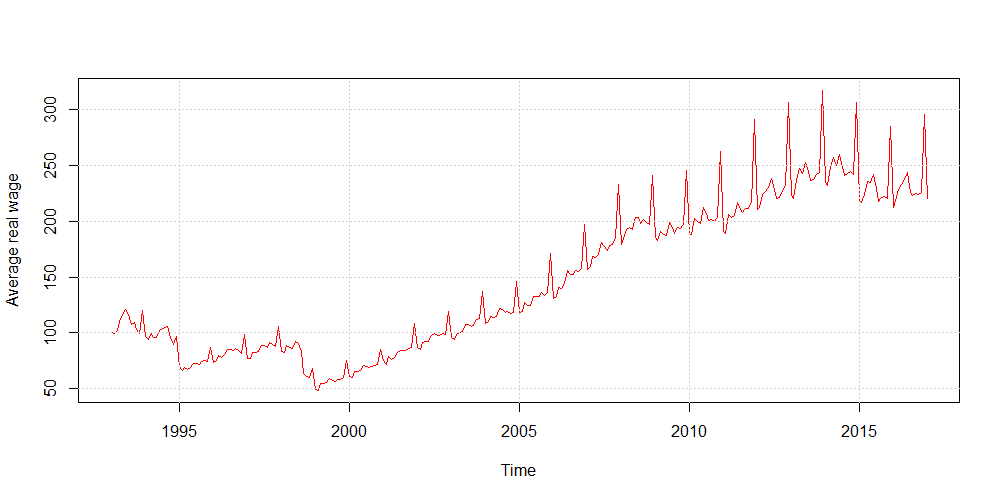
\includegraphics[width=0.65\textwidth]{wage.png}
	\end{center}
	
	Задача прогнозирования~--- найти функцию $f_T\colon$
	$$y_{T+d} \approx f_T\left(y_T,\dots,y_1,d\right) \equiv \hat{y}_{T+d|T},$$
	где $d \in \left\{1,\dots,D\right\}$~--- отсрочка прогноза, $D$~--- горизонт прогнозирования.		
\end{frame}

\subsection{Особенности задачи}
\begin{frame}{Регрессия}
%%%%%%%%%%%%%%%%%%%%%%%%%%%%%%%%%%%%%%%%%%%%%%%%%%%%%%%%%%%%%%%%%%%%%%%
% До этого, на протяжении практически всего курса, считалось, что анализируемые данные — это простые выборки, то есть независимые одинаково распределённые наблюдения. В задаче анализа временных рядов всё с точностью наоборот: предполагается, что данные в прошлом каким-то образом связаны с данными в будущем. Чем сильнее они связаны, тем больше имеется информации о поведении временного ряда в будущем и тем точнее можно сделать прогноз.
% Как этот прогноз построить? Мы хорошо умее делать регрессию. Процесс разворачивается во времени, поэтому кажется логичным задать признак, связанный со временем, и попробовать решить задачу, применяя модель регрессии. Признак может зависеть от вермени линейно, или например, квадратично.
% Однако это решение слишком простое, чтобы быть хорошим. Остатки такой регрессии (рис. 1.3) далеко не похожи на случайный шум, в них остаётся большая часть структуры, которая не была учтена в регрессионной модели. Чем больше структуры временного ряда учитывается в модели, тем лучшее предсказание она даёт. Вид остатков регрессии намекает на то, что можно построить более сложную модель, которая будет лучше описывать имеющиеся данные, а также давать более точные прогнозы в будущем.
%%%%%%%%%%%%%%%%%%%%%%%%%%%%%%%%%%%%%%%%%%%%%%%%%%%%%%%%%%%%%%%%%%%%%%%
	Простейшая идея: сделать регрессию на время.
	\begin{center}
		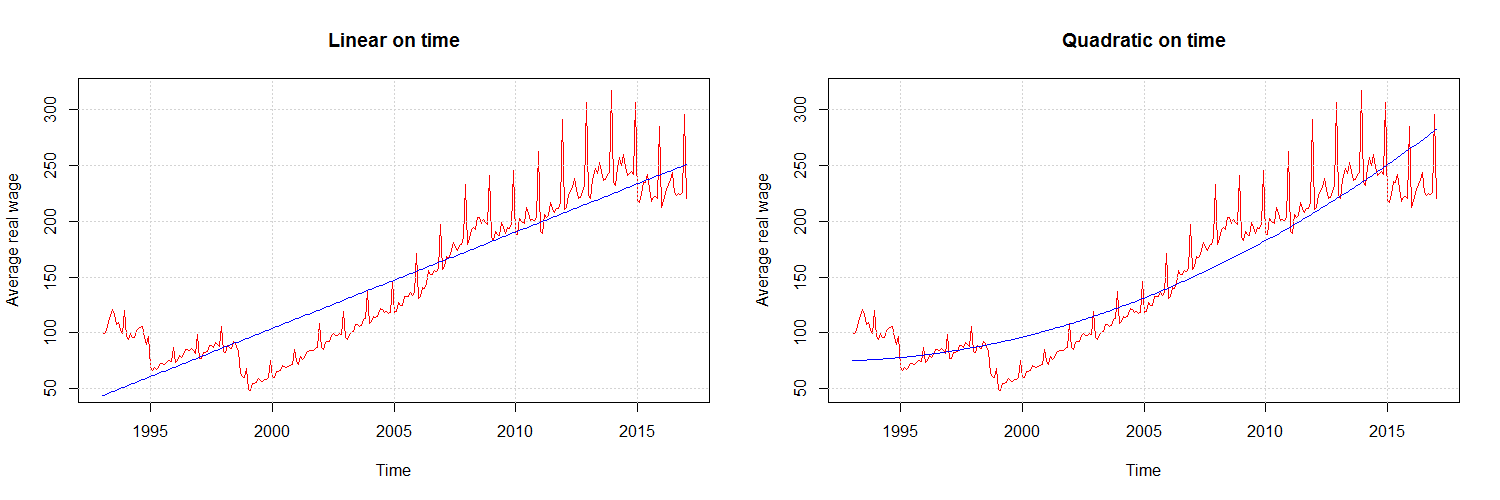
\includegraphics[width=0.7\textwidth]{wage1.png}
	\end{center}		
	
	Остатки не выглядят как шум:
	\begin{center}
		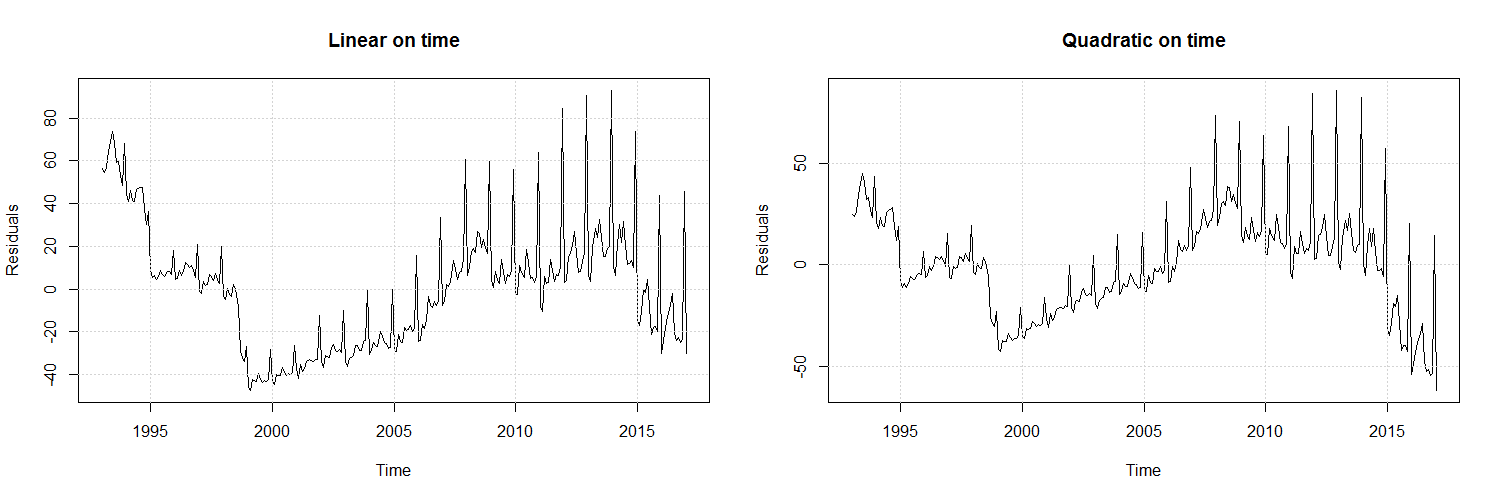
\includegraphics[width=0.7\textwidth]{wage2.png}
	\end{center}			
\end{frame}

\begin{frame}{Продажи вина в Австралии}
%%%%%%%%%%%%%%%%%%%%%%%%%%%%%%%%%%%%%%%%%%%%%%%%%%%%%%%%%%%%%%%%%%%%%%%
% Одной из важнейших характеристик временного ряда является автокорреляция. Далее суть этой характеристики будет демонстрироваться на примере данных о суммарном объёме продаж вина в Австралии за месяц на протяжении почти 15 лет. Этот ряд обладает ярко выраженной годовой сезонностью: максимум продаж за год приходится на декабрь, а затем, в январе, происходит существенное падение.
%%%%%%%%%%%%%%%%%%%%%%%%%%%%%%%%%%%%%%%%%%%%%%%%%%%%%%%%%%%%%%%%%%%%%%%
	\begin{center}
		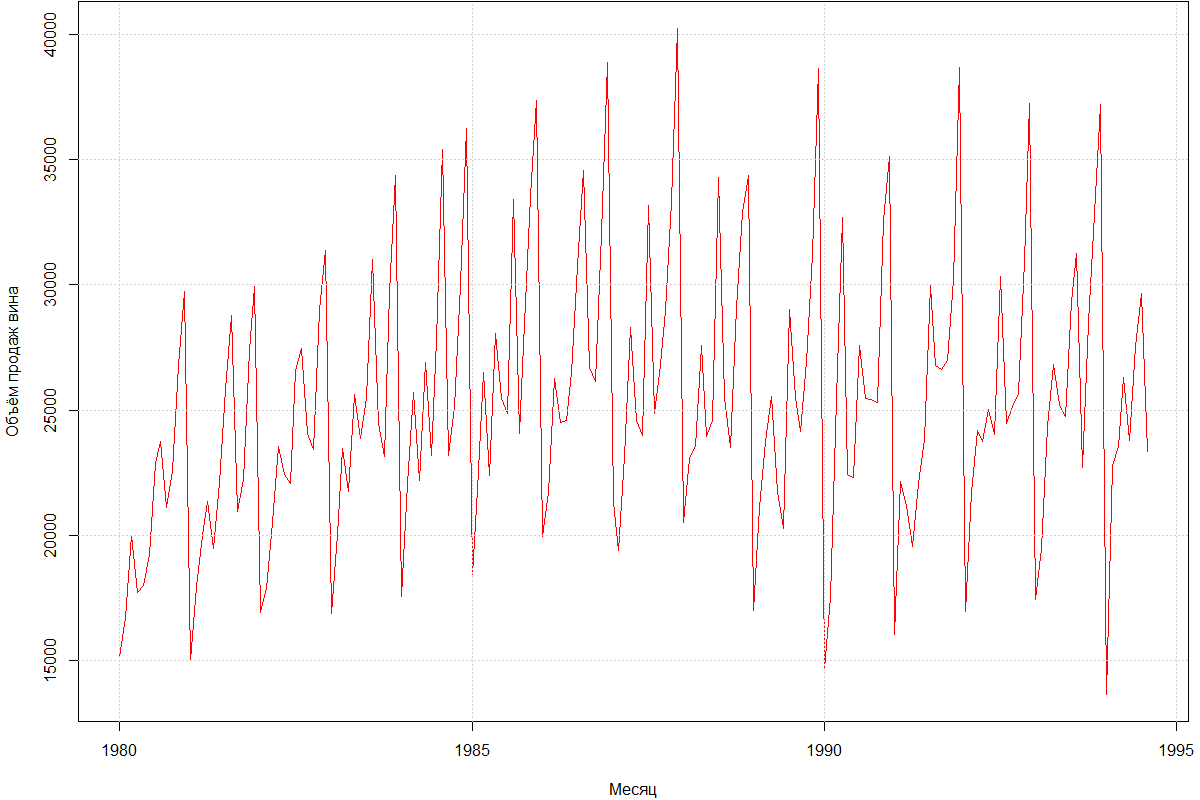
\includegraphics[width=0.8\textwidth]{wine.png}
	\end{center}	
\end{frame}

\begin{frame}{Продажи в соседние месяцы}
%%%%%%%%%%%%%%%%%%%%%%%%%%%%%%%%%%%%%%%%%%%%%%%%%%%%%%%%%%%%%%%%%%%%%%%
% На рисунке показано, как связаны объёмы продаж вина в соседние месяцы. Видно, что большая часть точек на графике группируется вокруг главной диагонали. Это говорит о том, что в основном значения продаж в соседние месяцы похожи. Ещё одно подмножество точек выделяется в правом нижнем углу, оно связано с падением продаж от декабря к январю, которое было видно на предыдущем графике.
%%%%%%%%%%%%%%%%%%%%%%%%%%%%%%%%%%%%%%%%%%%%%%%%%%%%%%%%%%%%%%%%%%%%%%%
	\begin{center}
		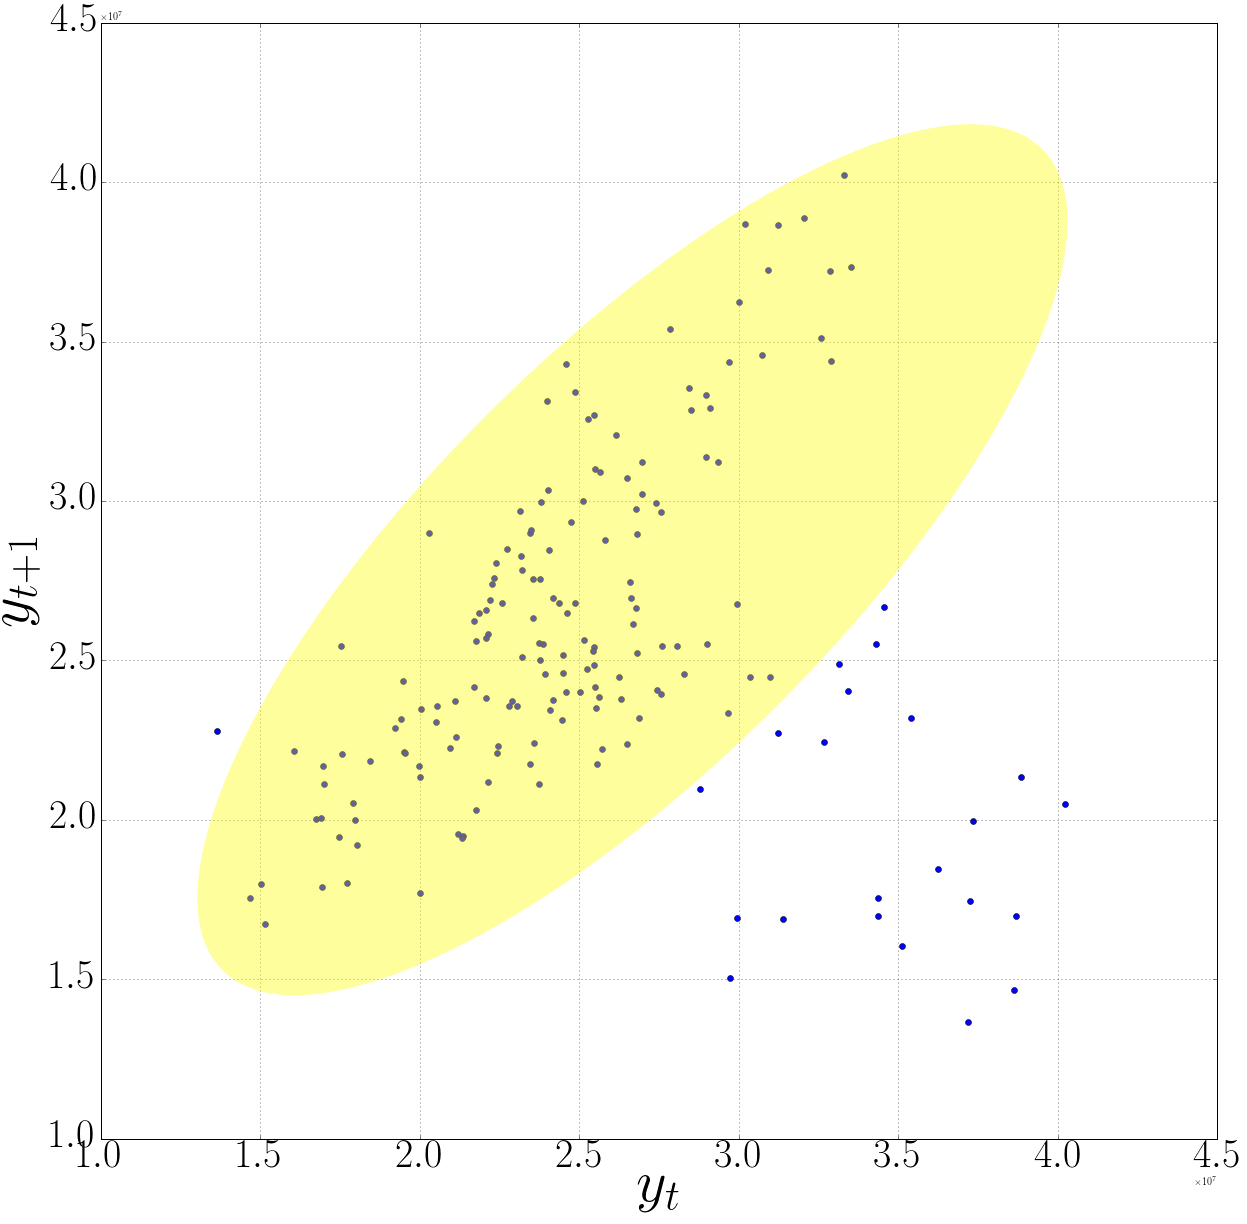
\includegraphics[height=0.6\textheight]{wine5.png}
	\end{center}
\end{frame}

\begin{frame}{Продажи через 1 месяц}
%%%%%%%%%%%%%%%%%%%%%%%%%%%%%%%%%%%%%%%%%%%%%%%%%%%%%%%%%%%%%%%%%%%%%%%
% Если построить аналогичный график, но по вертикальной оси отложить y_{t+2}, то видно, что точки в основном облаке начинают ”расплываться” вокруг главной диагонали, то есть сходство между продажами через месяц уменьшается по сравнению с соседними месяцами.
%%%%%%%%%%%%%%%%%%%%%%%%%%%%%%%%%%%%%%%%%%%%%%%%%%%%%%%%%%%%%%%%%%%%%%%
	\begin{center}
		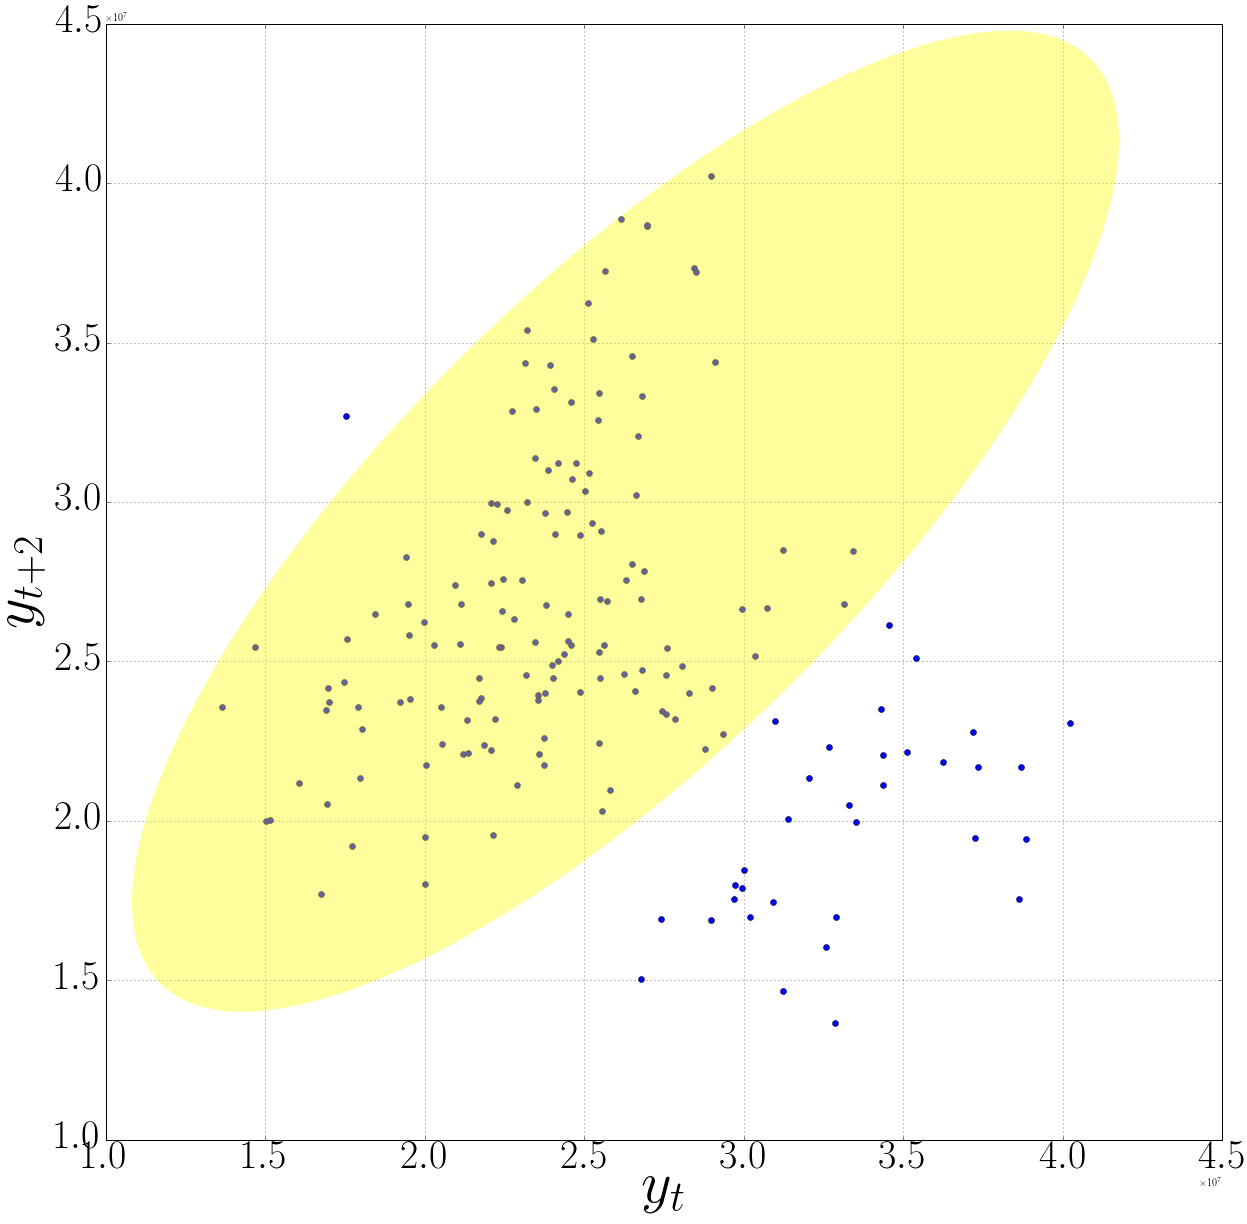
\includegraphics[height=0.6\textheight]{wine7.png}
	\end{center}
\end{frame}

\begin{frame}{Продажи через 2 месяца}
%%%%%%%%%%%%%%%%%%%%%%%%%%%%%%%%%%%%%%%%%%%%%%%%%%%%%%%%%%%%%%%%%%%%%%%
% Если посмотреть связь между продажами через два месяца, то облако станет ещё шире, а сходство — ещё меньше.
%%%%%%%%%%%%%%%%%%%%%%%%%%%%%%%%%%%%%%%%%%%%%%%%%%%%%%%%%%%%%%%%%%%%%%%
	\begin{center}
		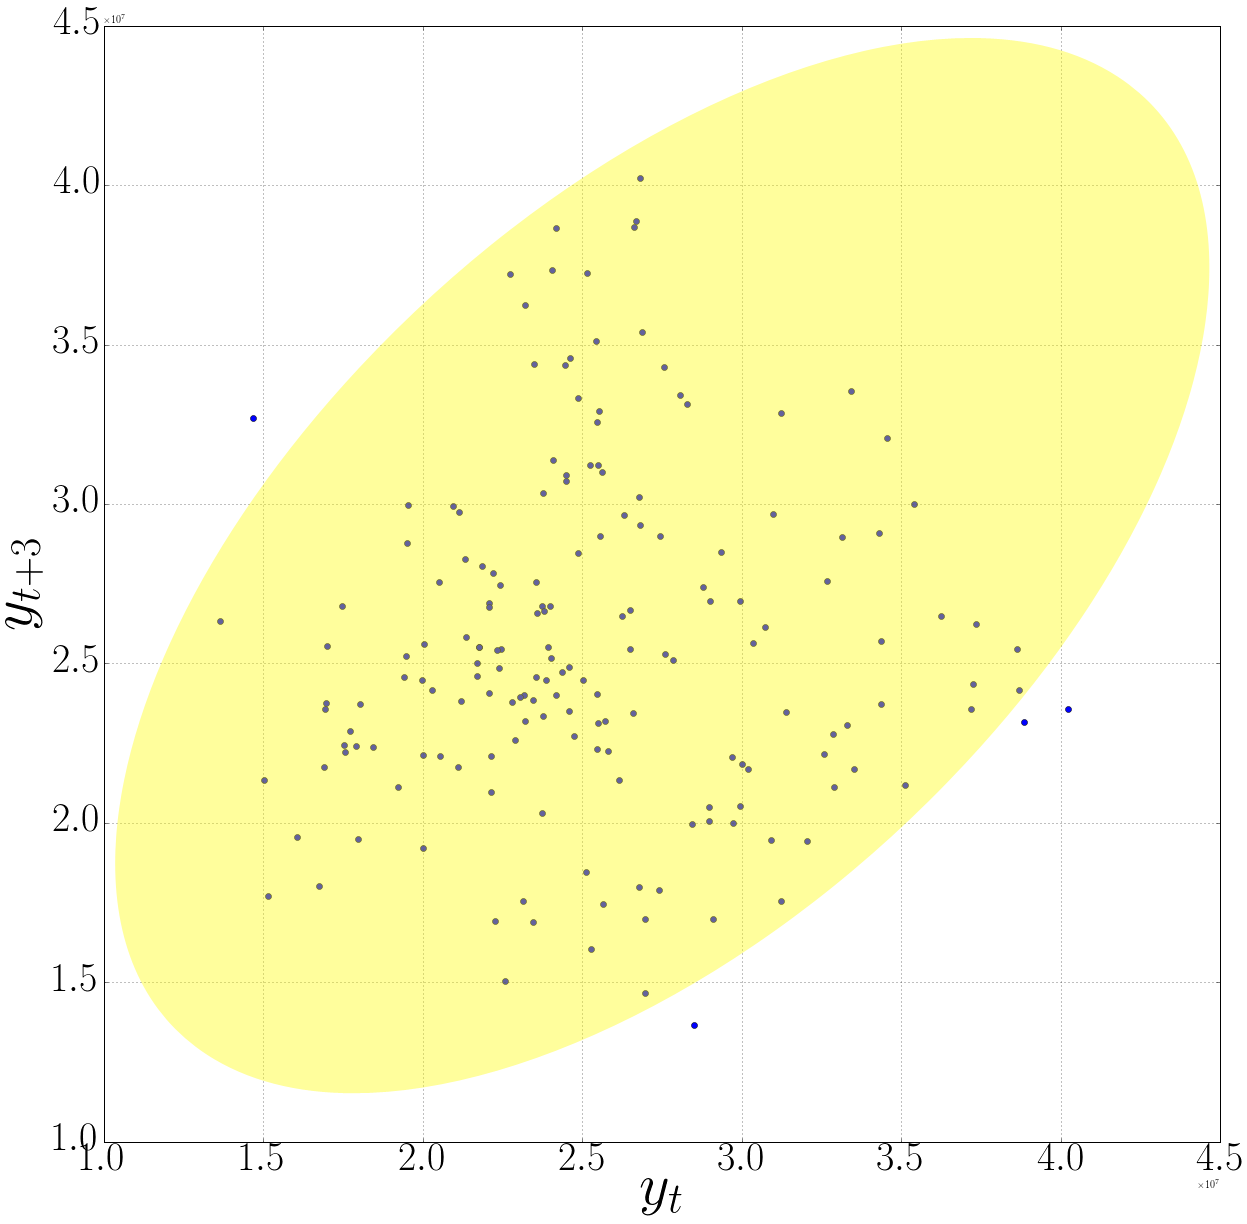
\includegraphics[height=0.6\textheight]{wine8.png}
	\end{center}
\end{frame}

\begin{frame}{Продажи через год}
%%%%%%%%%%%%%%%%%%%%%%%%%%%%%%%%%%%%%%%%%%%%%%%%%%%%%%%%%%%%%%%%%%%%%%%
% Однако если рассмотреть продажи в одни и те же месяцы соседних лет, то видно, что точки на графике снова стягиваются к главной диагонали. Это значит, что значения продаж в одни и те же месяцы соседних лет очень сильно похожи.
%%%%%%%%%%%%%%%%%%%%%%%%%%%%%%%%%%%%%%%%%%%%%%%%%%%%%%%%%%%%%%%%%%%%%%%
	\begin{center}
		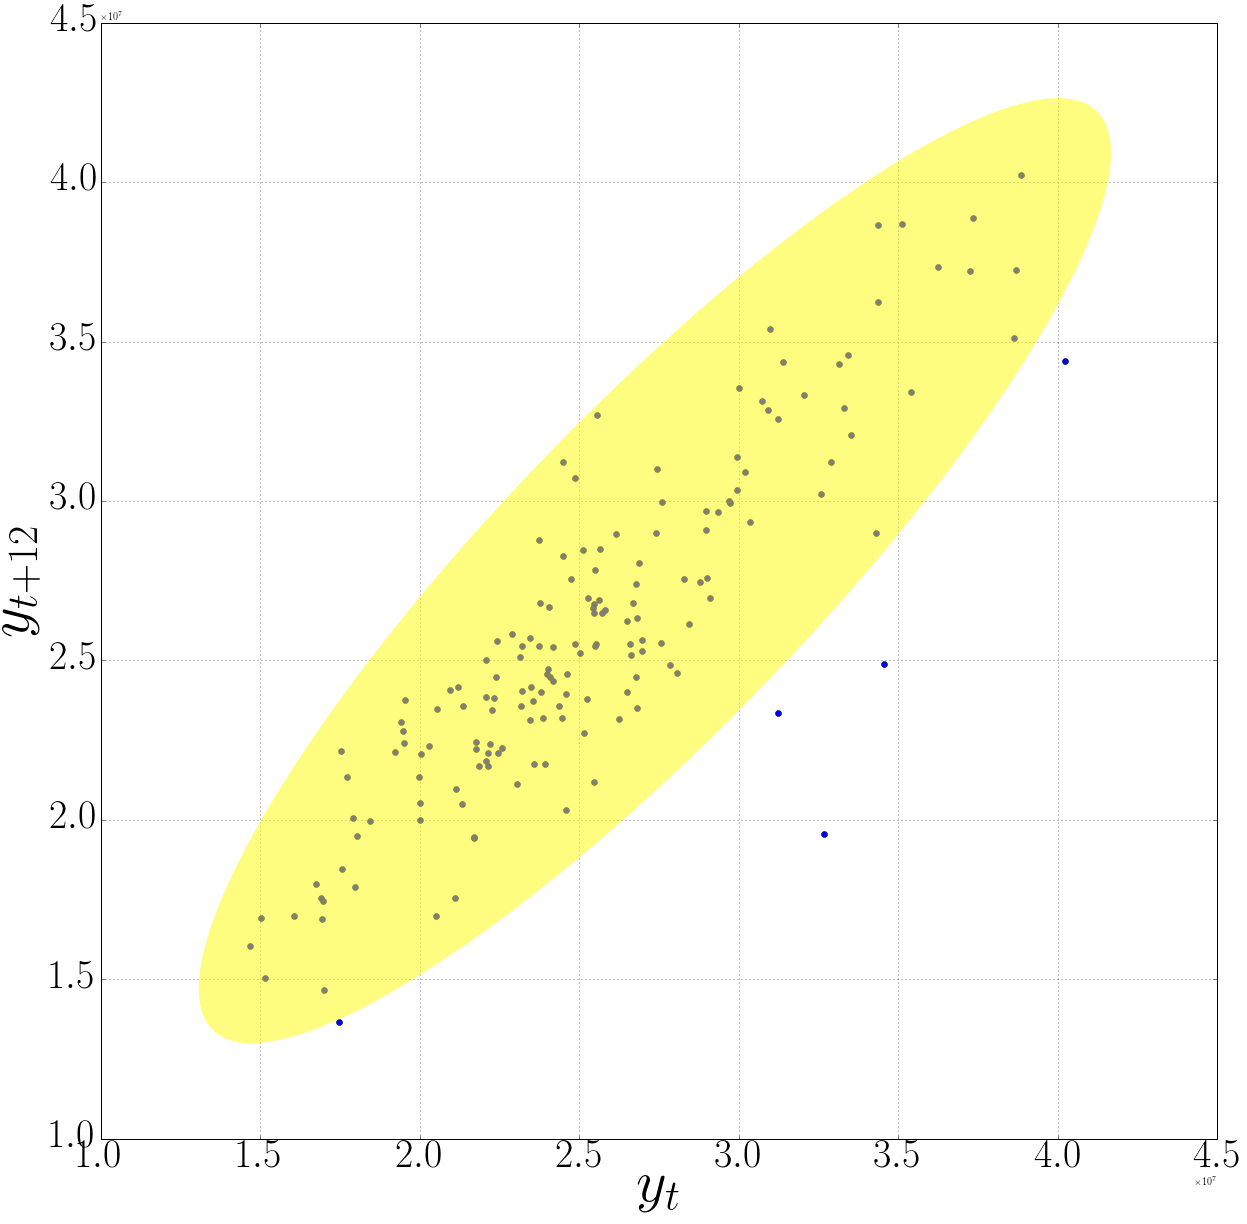
\includegraphics[height=0.6\textheight]{wine9.png}
	\end{center}
\end{frame}

\begin{frame}{Автокорреляционная функция (ACF)}
%%%%%%%%%%%%%%%%%%%%%%%%%%%%%%%%%%%%%%%%%%%%%%%%%%%%%%%%%%%%%%%%%%%%%%%
% Одной из важнейших характеристик временного ряда является автокорреляция, измеряющая в каком-то смысле сходство между значениями ряда в соседних точках. Автокорреляция — это уже встречавшаяся ранее корреляция Пирсона между исходным рядом и его версией, сдвинутой на несколько отсчётов. Количество отсчётов, на которое сдвинут ряд, называется лагом автокорреляции. Значения, принимаемые автокорреляцией такие же, как и у коэффициента Пирсона: [-1; 1]. Проверить, значимо ли отличие автокорреляции от нуля, можно с помощью такого же критерия Стьюдента, как используется для корреляции Пирсона.
%%%%%%%%%%%%%%%%%%%%%%%%%%%%%%%%%%%%%%%%%%%%%%%%%%%%%%%%%%%%%%%%%%%%%%%
	\only<1>{
	Наблюдения временного ряда автокоррелированы.
	
	\bigskip	
		
		\textbf{Автокорреляция:}
		$$r_\tau = r_{y_t y_{t+\tau}} = \frac{\sum\limits_{t=1}^{T-\tau} \left(y_t - \bar{y}\right)\left(y_{t+\tau} - \bar{y}\right) }{ \sum\limits_{t=1}^T \left(y_t - \bar{y}\right)^2 },\;\; \bar{y} = \frac1{T} \sum_{t=1}^T y_t.$$
		
		$r_\tau \in\left[-1,1\right], \;\; \tau$~--- лаг автокорреляции.
		
		\bigskip
		
		Проверка значимости отличия автокорреляции от нуля:
		\begin{center}
			\begin{tabular}{rl}
				временной ряд:                  & $Y^T = Y_1,\dots,Y_T;$ \\
				нулевая гипотеза:               & $H_0\colon r_\tau=0;$ \\
				альтернатива:                   & $H_1\colon r_\tau\neq0;$ \\
				статистика:                     & $T\left(Y^T\right) = \frac{r_{\tau} \sqrt{T-\tau-2}}{\sqrt{1-r_\tau^2}};$ \\
				нулевое распределение:          & $St\left(T-\tau-2\right)$.\\
			\end{tabular}
		\end{center}
	}
	
	\only<2>{
		Коррелограмма:
		\begin{center}
			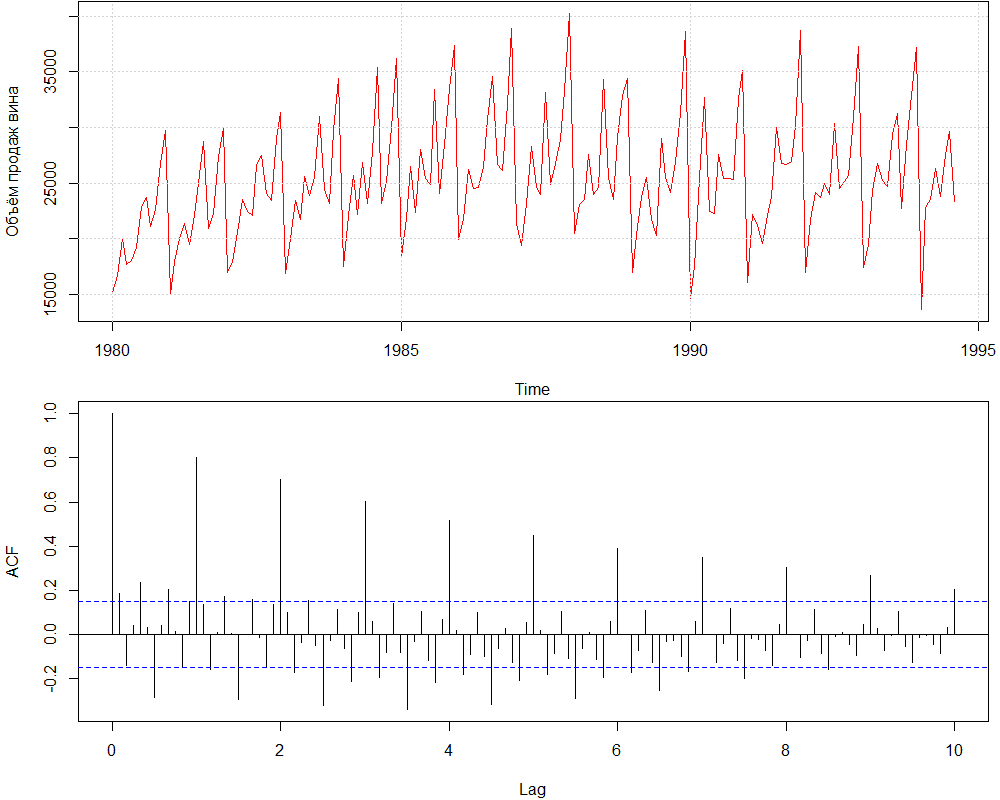
\includegraphics[height=0.85\textheight]{wineacf.png}
		\end{center}				
	}
\end{frame}


\begin{frame}{Компоненты временных рядов}
%%%%%%%%%%%%%%%%%%%%%%%%%%%%%%%%%%%%%%%%%%%%%%%%%%%%%%%%%%%%%%%%%%%%%%%
% Полезно рассмотреть несколько понятий, которыми можно описать поведение временных рядов:
% Тренд — плавное долгосрочное изменение уровня ряда. Эту характеристику можно оценить, наблюдая ряд в течение достаточно долгого времени.
% Сезонность — циклические изменения уровня ряда с постоянным периодом. В данных о средней зарплате в России очень хорошо видны подобные сезонные колебания: признак всегда принимает максимальное значение в декабре каждого года, а минимальное — в январе следующего года. В целом профиль изменения зарплаты внутри года остаётся более-менее постоянным.
% Цикл — изЁменение уровня ряда с переменным периодом. Такое поведение часто встречается в рядах, связанных с продажами, и объясняется циклическими изменениями экономической активности. В экономике выделяют циклы длиной 4 - 5 лет, 7 - 11 лет, 45 - 50 лет и т. д. Другой пример ряда с такой характеристикой — это солнечная активность, которая соответствует, например, количеству солнечных пятен за день. Она плавно меняется с периодом, который составляет несколько лет, причём сам период также меняется во времени.
% Ошибка — непрогнозируемая случайная компонента ряда. Сюда включены все те характеристики временного ряда, которые сложно измерить (например, слишком слабые).
%%%%%%%%%%%%%%%%%%%%%%%%%%%%%%%%%%%%%%%%%%%%%%%%%%%%%%%%%%%%%%%%%%%%%%%
	\only<1>{
		\textbf{Тренд}~--- плавное долгосрочное изменение уровня ряда.
		
		\bigskip
		
		\textbf{Сезонность}~--- циклические изменения уровня ряда с постоянным периодом.
		
		\bigskip
		
		\textbf{Цикл}~--- изменения уровня ряда с переменным периодом (цикл жизни товара, экономические волны, периоды солнечной активности).
		
		\bigskip
		
		\textbf{Ошибка}~--- непрогнозируемая случайная компонента ряда.
	}

	\only<2>{
%%%%%%%%%%%%%%%%%%%%%%%%%%%%%%%%%%%%%%%%%%%%%%%%%%%%%%%%%%%%%%%%%%%%%%%
% Левый верхний график - суммарный объём проданной жилой недвижимости в Америке за месяц, данные собраны за несколько лет. На графике наблюдается сочетание двух основных компонент. Первая компонента — это годовая сезонность (минимум всегда приходится на зиму, а максимум — на середину лета), а вторая — это циклы, связанные с изменением среднего уровня экономической активности (период в данном случае составляет 7-9 лет).
% Правый верхний график - количество контрактов за день в сокровищнице США. На графике виден хорошо выраженный понижающийся тренд, который можно описать линейной функцией. На этом участке в данных не наблюдается ни циклов, ни сезонности. По-видимому, всё, что не удаётся описать трендом, является ошибкой.
% Слева внизу данные за несколько лет о суммарном объёме электричества, произведённого за месяц в Австралии. На графике, как и в предыдущем случае, виден тренд, на этот раз повышающийся. Кроме того, наблюдается годовая сезонность: значение признака совершает колебания, минимум которых всегда приходится на зиму, а максимум — на середину лета. Это легко объяснить тем, что зимой электричества необходимо меньше всего, это самый тёплый сезон в Австралии.
% Справа внизу ежедневные изменения индекса Доу-Джонса. Глядя на этот график, сложно сказать, присутствует ли в данных какая-то систематическая компонента: явно нет ни тренда, ни сезонности, ни цикла. По всей видимости, ряд представляет собой что-то похожее на случайные колебания. Однако даже такие ряды можно прогнозировать.
%%%%%%%%%%%%%%%%%%%%%%%%%%%%%%%%%%%%%%%%%%%%%%%%%%%%%%%%%%%%%%%%%%%%%%%
		\begin{center}
			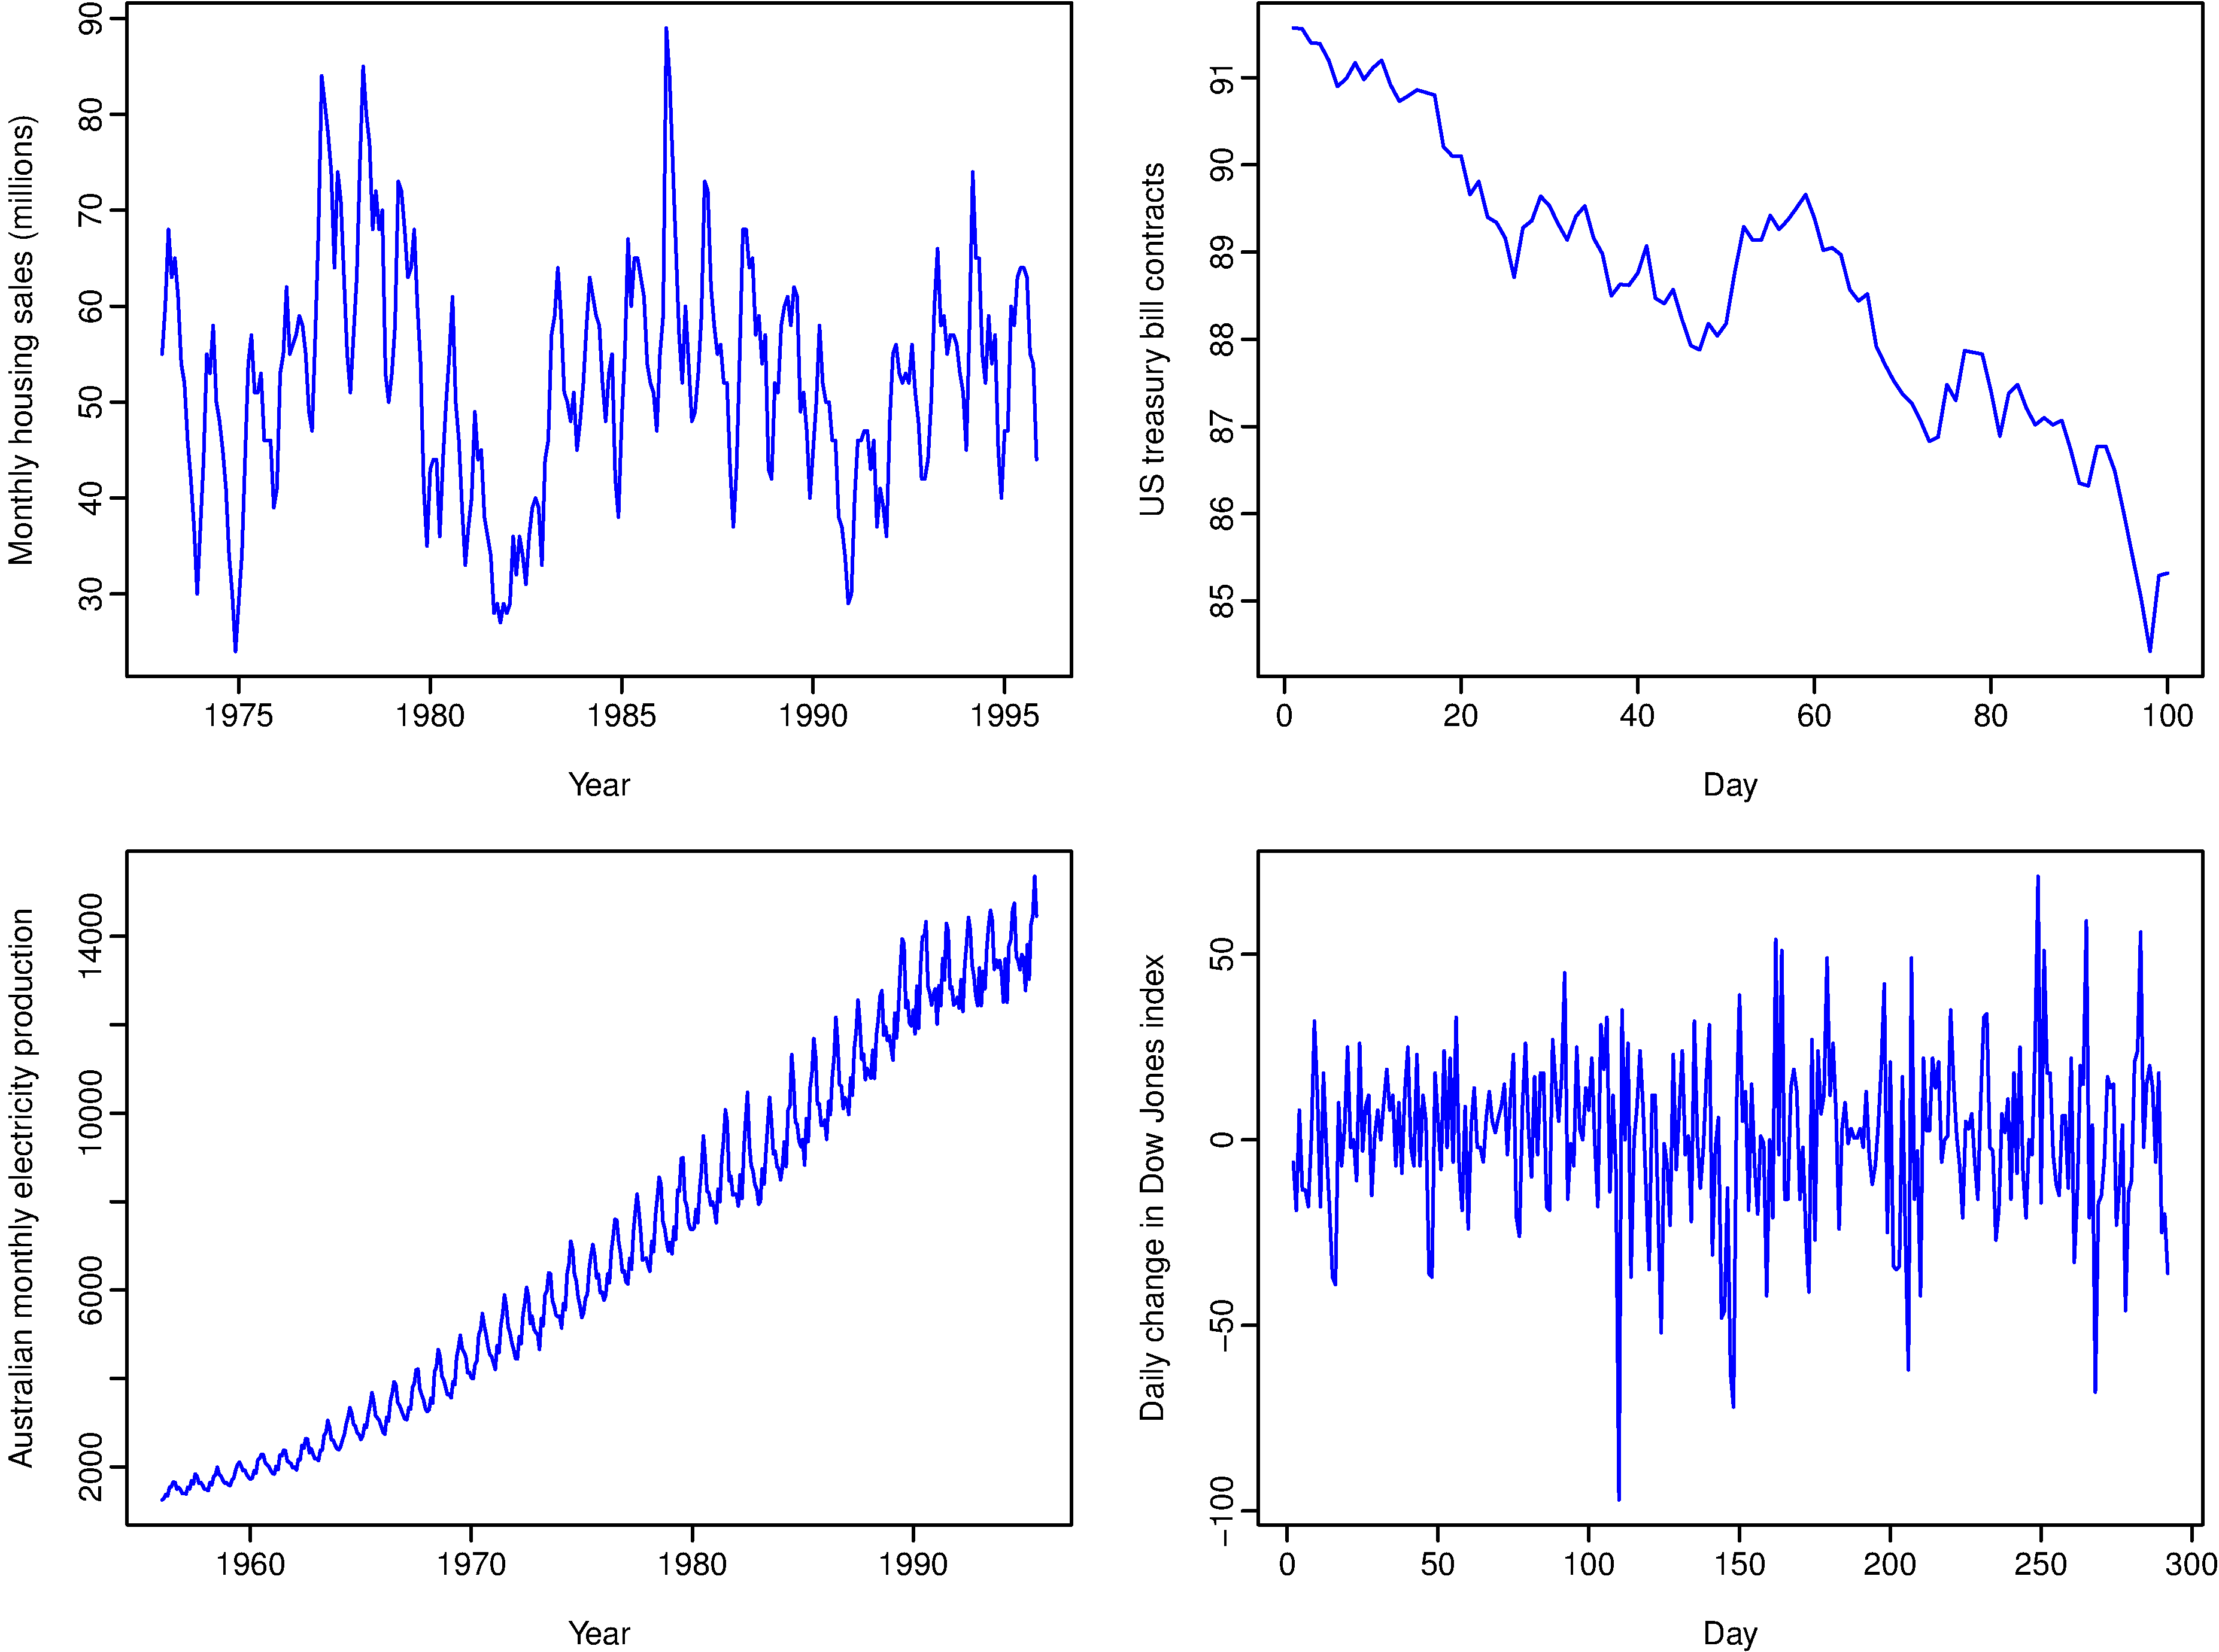
\includegraphics[width=0.7\textwidth]{decomp1.png}
		\end{center}		
	}
	
	\only<3>{
%%%%%%%%%%%%%%%%%%%%%%%%%%%%%%%%%%%%%%%%%%%%%%%%%%%%%%%%%%%%%%%%%%%%%%%
% Давайте теперь посмотрим, как на коррелограммах проявляются разные компоненты временных рядов. Вернёмся к коррелограмме ряда продаж вина в Австралии. На графике видно, что автокорреляция принимает большие значения в лагах, кратных сезонному периоду. Такой вид коррелограммы типичен для данных с выраженной сезонностью.
%%%%%%%%%%%%%%%%%%%%%%%%%%%%%%%%%%%%%%%%%%%%%%%%%%%%%%%%%%%%%%%%%%%%%%%
		\begin{center}
			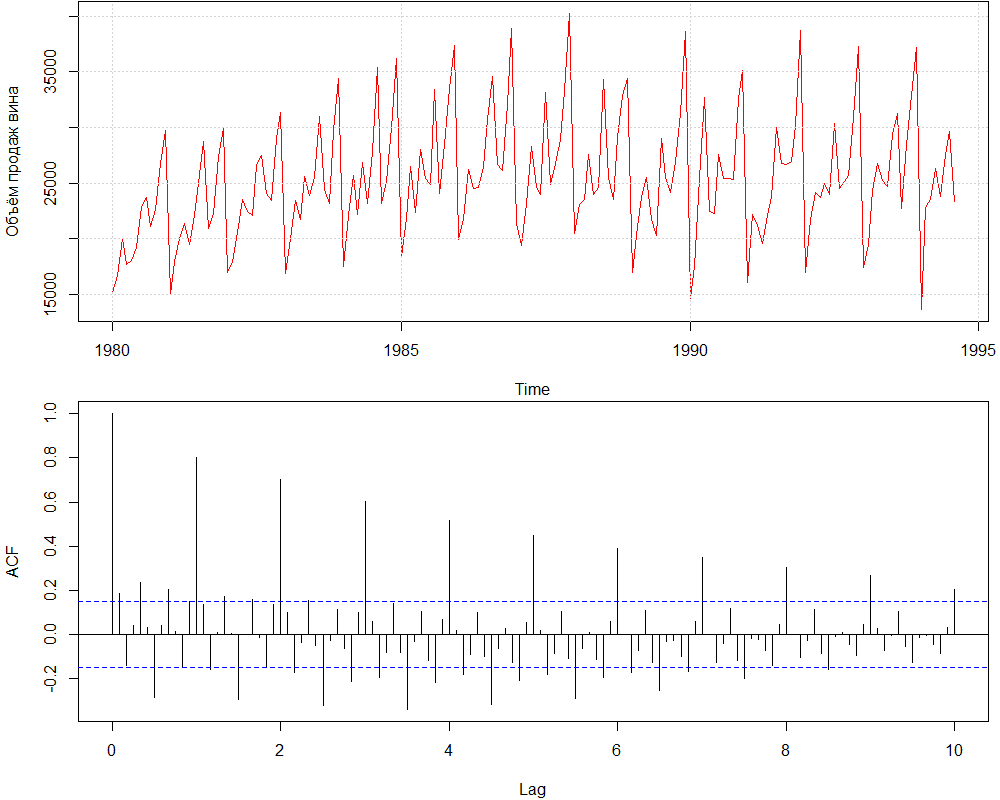
\includegraphics[height=0.7\textheight]{wineacf.png}
		\end{center}				
	}
	\only<4>{	
%%%%%%%%%%%%%%%%%%%%%%%%%%%%%%%%%%%%%%%%%%%%%%%%%%%%%%%%%%%%%%%%%%%%%%%
% На этом слайде коррелограммы для четырёх только что рассмотренных рядов.
% Левый верхний график - типичная коррелограмма для ряда, в котором есть и сезонность, и цикл. Для самого первого лага, кратного сезонному периоду, виден пик, однако далее положение этого пика смещается: следующий пик не приходится на 2, 3 или 4 года. Это происходит, потому что в ряде есть циклы, период которых плавно меняется.
% Правый верхний график - типичная коррелограмма для данных с ярко выраженным трендом. Автокорреляция тем больше, чем меньше величина лага, и с ростом лага она начинает постепенно убывать, при  этом автокорреляция может начать колебаться вокруг горизонтальной оси, соответствующей её нулевому значению.
% В ряде слева внизу в котором присутствуют и тренд, и сезонность. Таким образом, на ней можно наблюдать оба описанных ранее эффекта, однако тренд настолько сильный, что практически нейтрализует влияние сезонности (следствие которой — наличие пиков в лагах, кратных периоду сезона).
% На коррелограмме, соответствующей данным о ежедневном изменении индекса Доу-Джонса, все значения автокорреляции невелики, кроме первого (в данной точке лаг = 0, и вычисляется корреляция значения ряда с самим собой, а такая корреляция всегда равна 1).
%%%%%%%%%%%%%%%%%%%%%%%%%%%%%%%%%%%%%%%%%%%%%%%%%%%%%%%%%%%%%%%%%%%%%%%	
		\begin{center}
			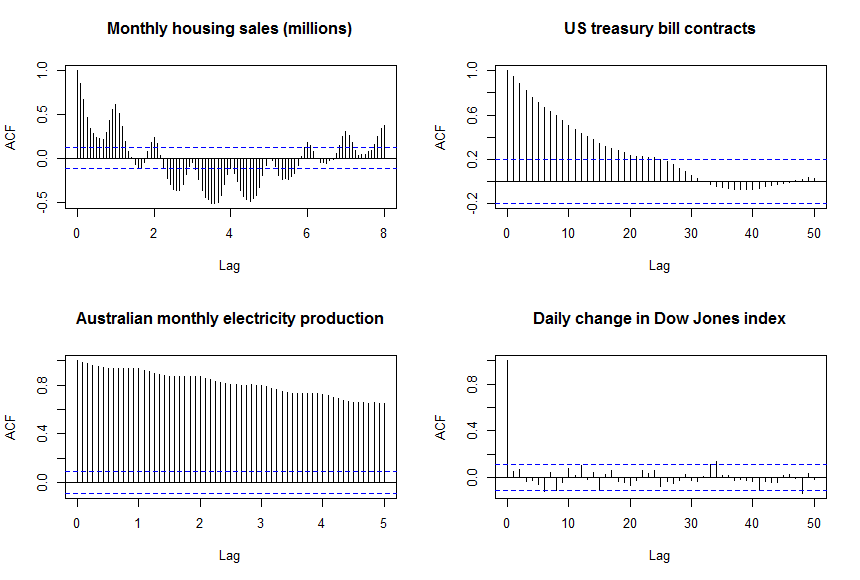
\includegraphics[width=0.8\textwidth]{acfs.png}
		\end{center}		
	}
	\only<5>{
%%%%%%%%%%%%%%%%%%%%%%%%%%%%%%%%%%%%%%%%%%%%%%%%%%%%%%%%%%%%%%%%%%%%%%%	
% STL-декомпозиция - простой эвристический метод оценки разных компонент временного ряда: на верхнем графике исходныя ряд, потом сезонность (ей разрешается немного меняться), потом тренд и ошибка.
%%%%%%%%%%%%%%%%%%%%%%%%%%%%%%%%%%%%%%%%%%%%%%%%%%%%%%%%%%%%%%%%%%%%%%%	
		STL-декомпозиция:
			\begin{center}
				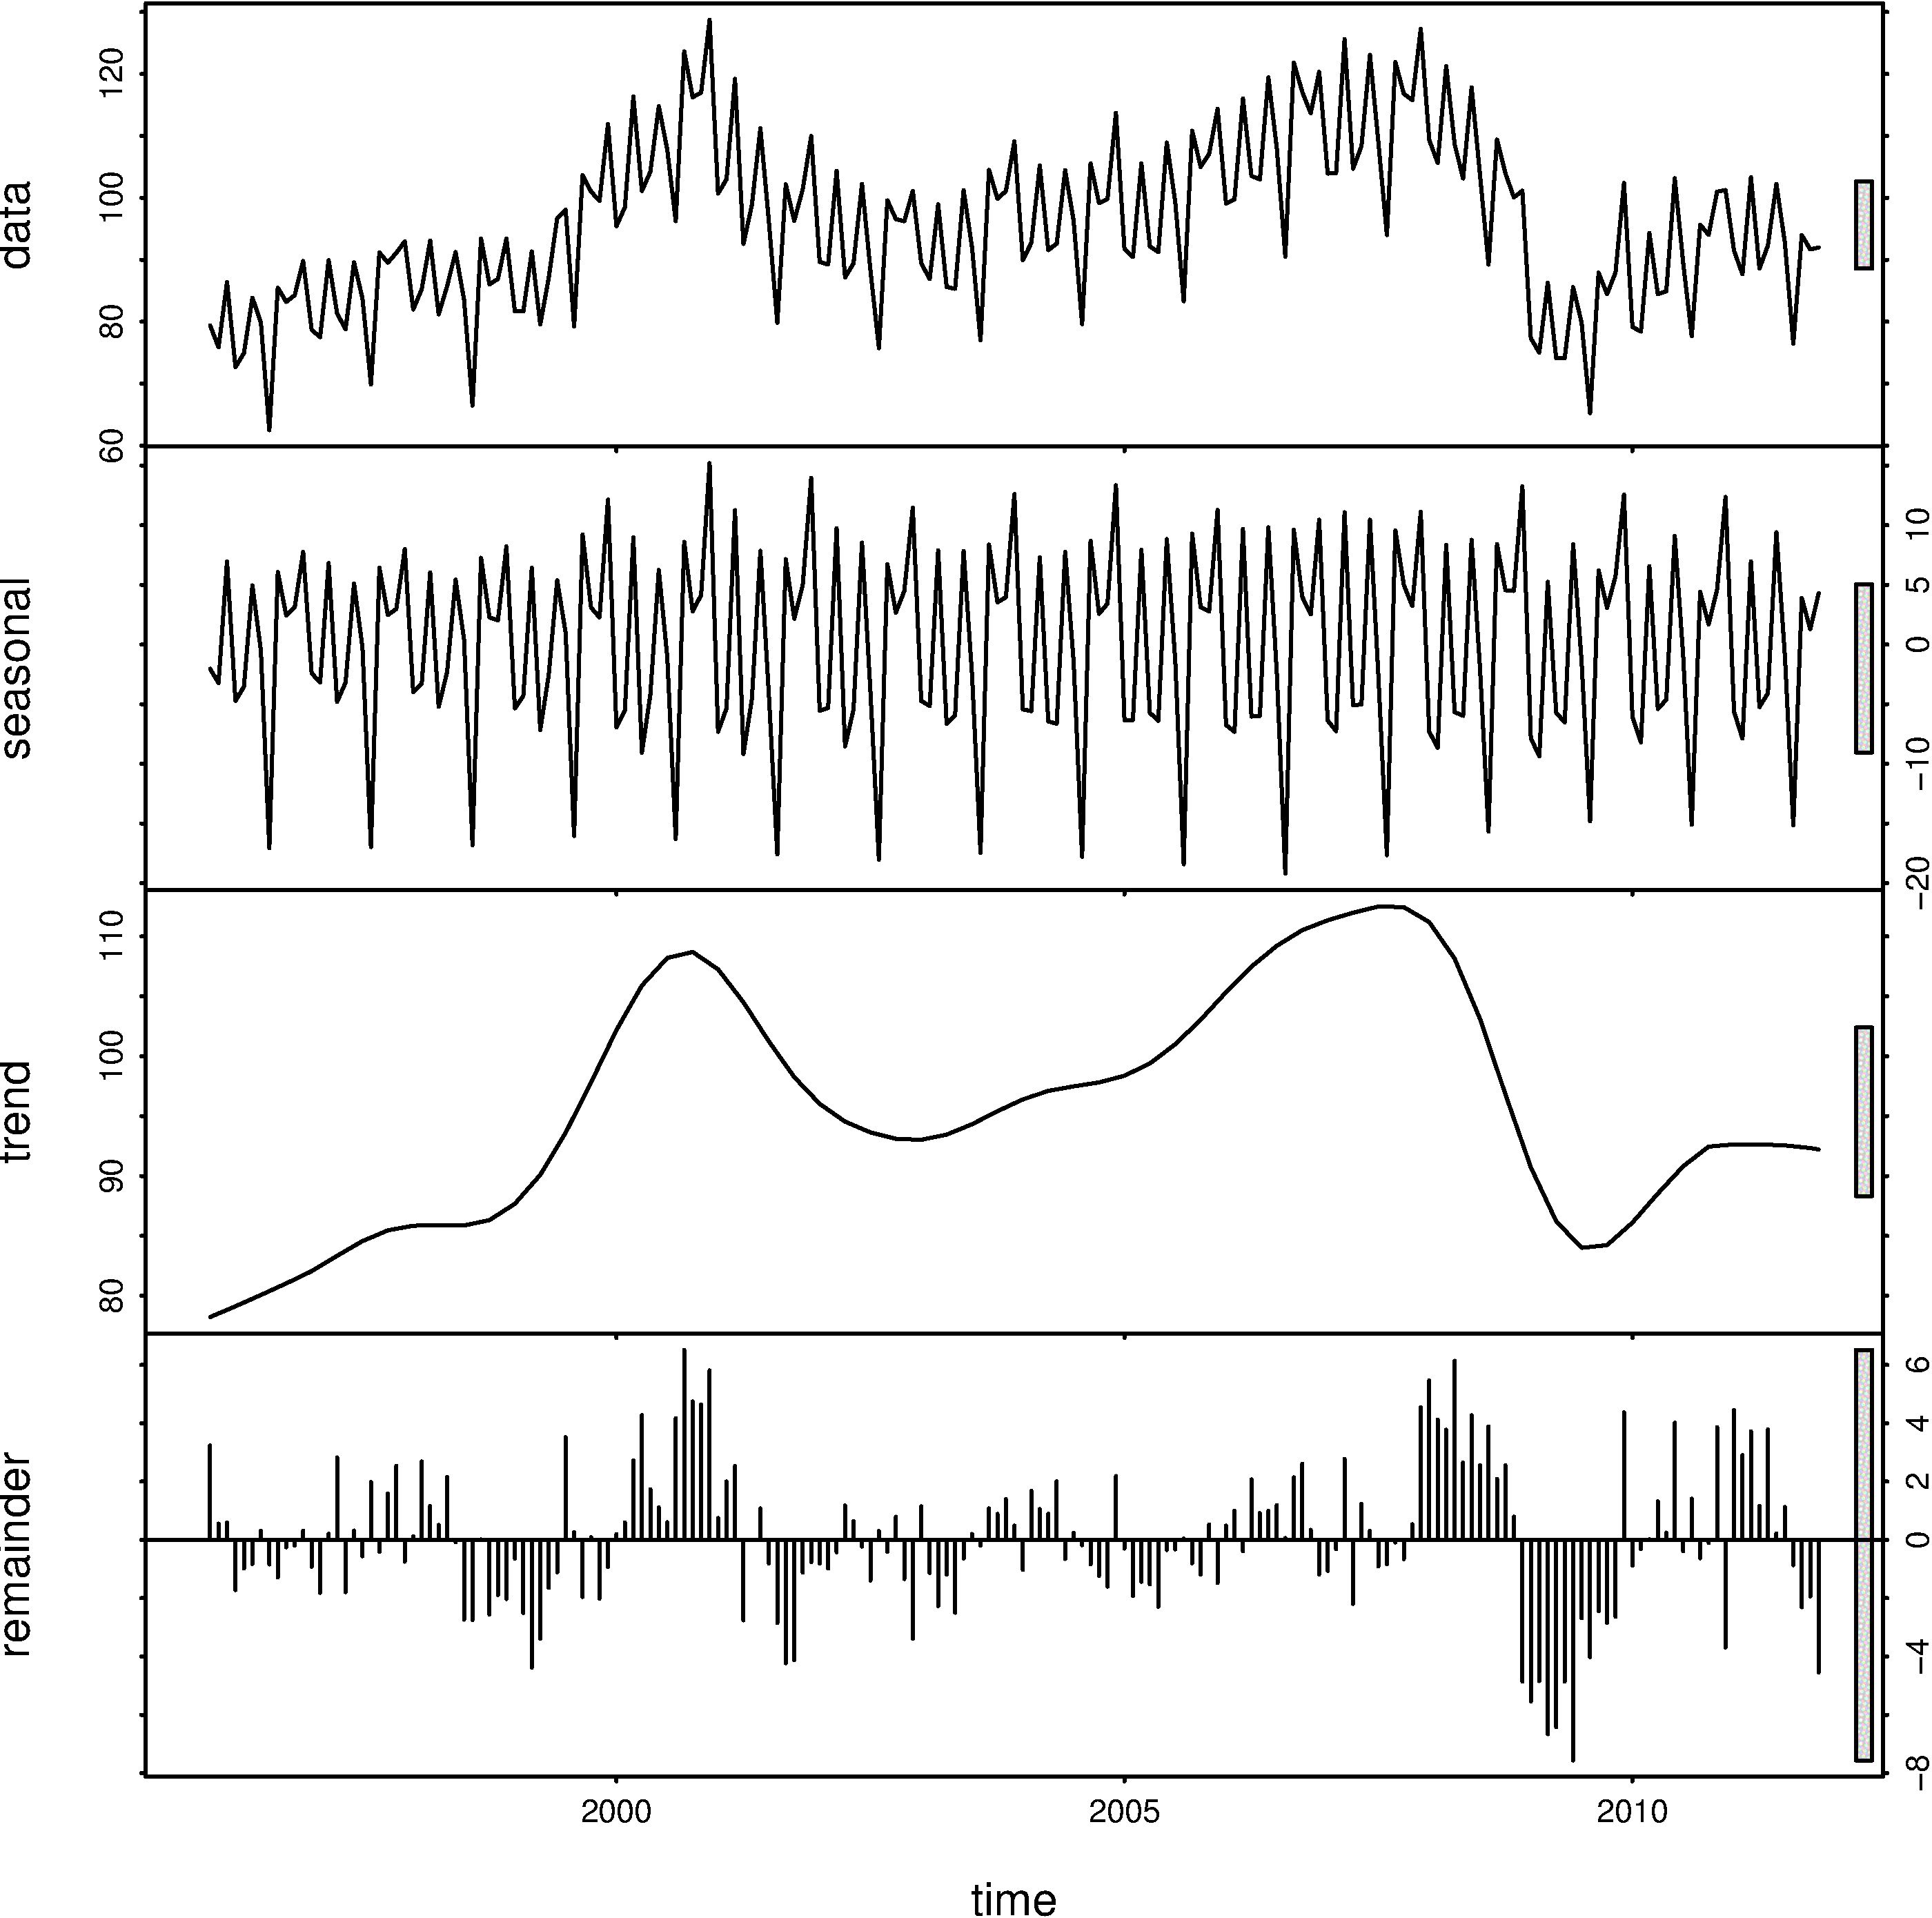
\includegraphics[height=0.6\textheight]{elecequip_stl.png}
			\end{center}			
	}
\end{frame}

\begin{frame}{Снятие сезонности}
	Часто для удобства интерпретации ряда сезонная компонента вычитается:	
	\begin{center}
		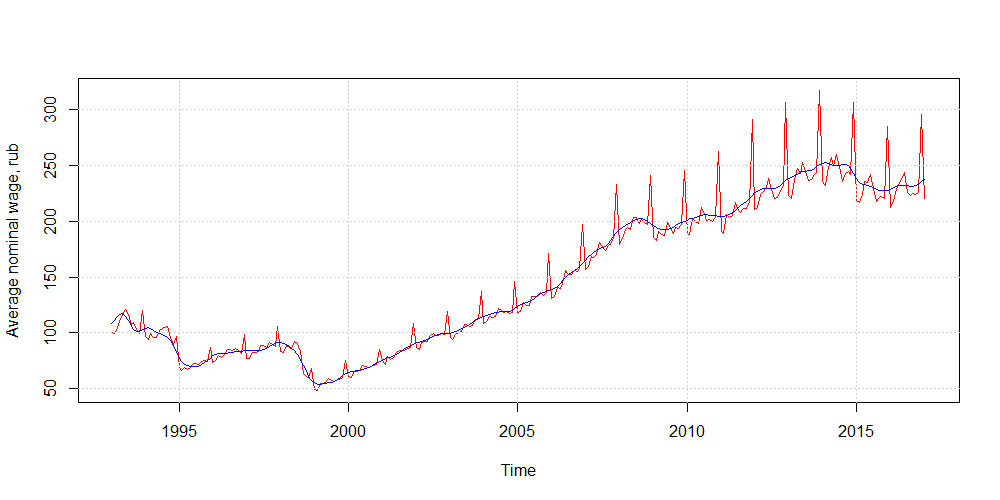
\includegraphics[width=.8\textwidth]{wageseas.png}
	\end{center}	
\end{frame}

\begin{frame}{Календарные эффекты}
%%%%%%%%%%%%%%%%%%%%%%%%%%%%%%%%%%%%%%%%%%%%%%%%%%%%%%%%%%%%%%%%%%%%%%%	
% Часто отсчёты временного ряда имеют разную абсолютную длину, например, если это месяцы. Если ряд имеет смысл суммарного количества чего-нибудь, то оказывается, что его структуру можно сильно упростить, если на эту длину поделить. Такой ряд оказывается проще прогнозировать, а в интерпретации мы при этом ничего не теряем. Иногда срабатывает деление не на количество дней, а на количество рабочих дней в периоде. Выбрать способ такого упрощения можно исходя из здравого смысла.
%%%%%%%%%%%%%%%%%%%%%%%%%%%%%%%%%%%%%%%%%%%%%%%%%%%%%%%%%%%%%%%%%%%%%%%	
	Иногда упростить структуру временного ряда можно за счёт учёта неравномерности отсчётов:
	
	\begin{center}
		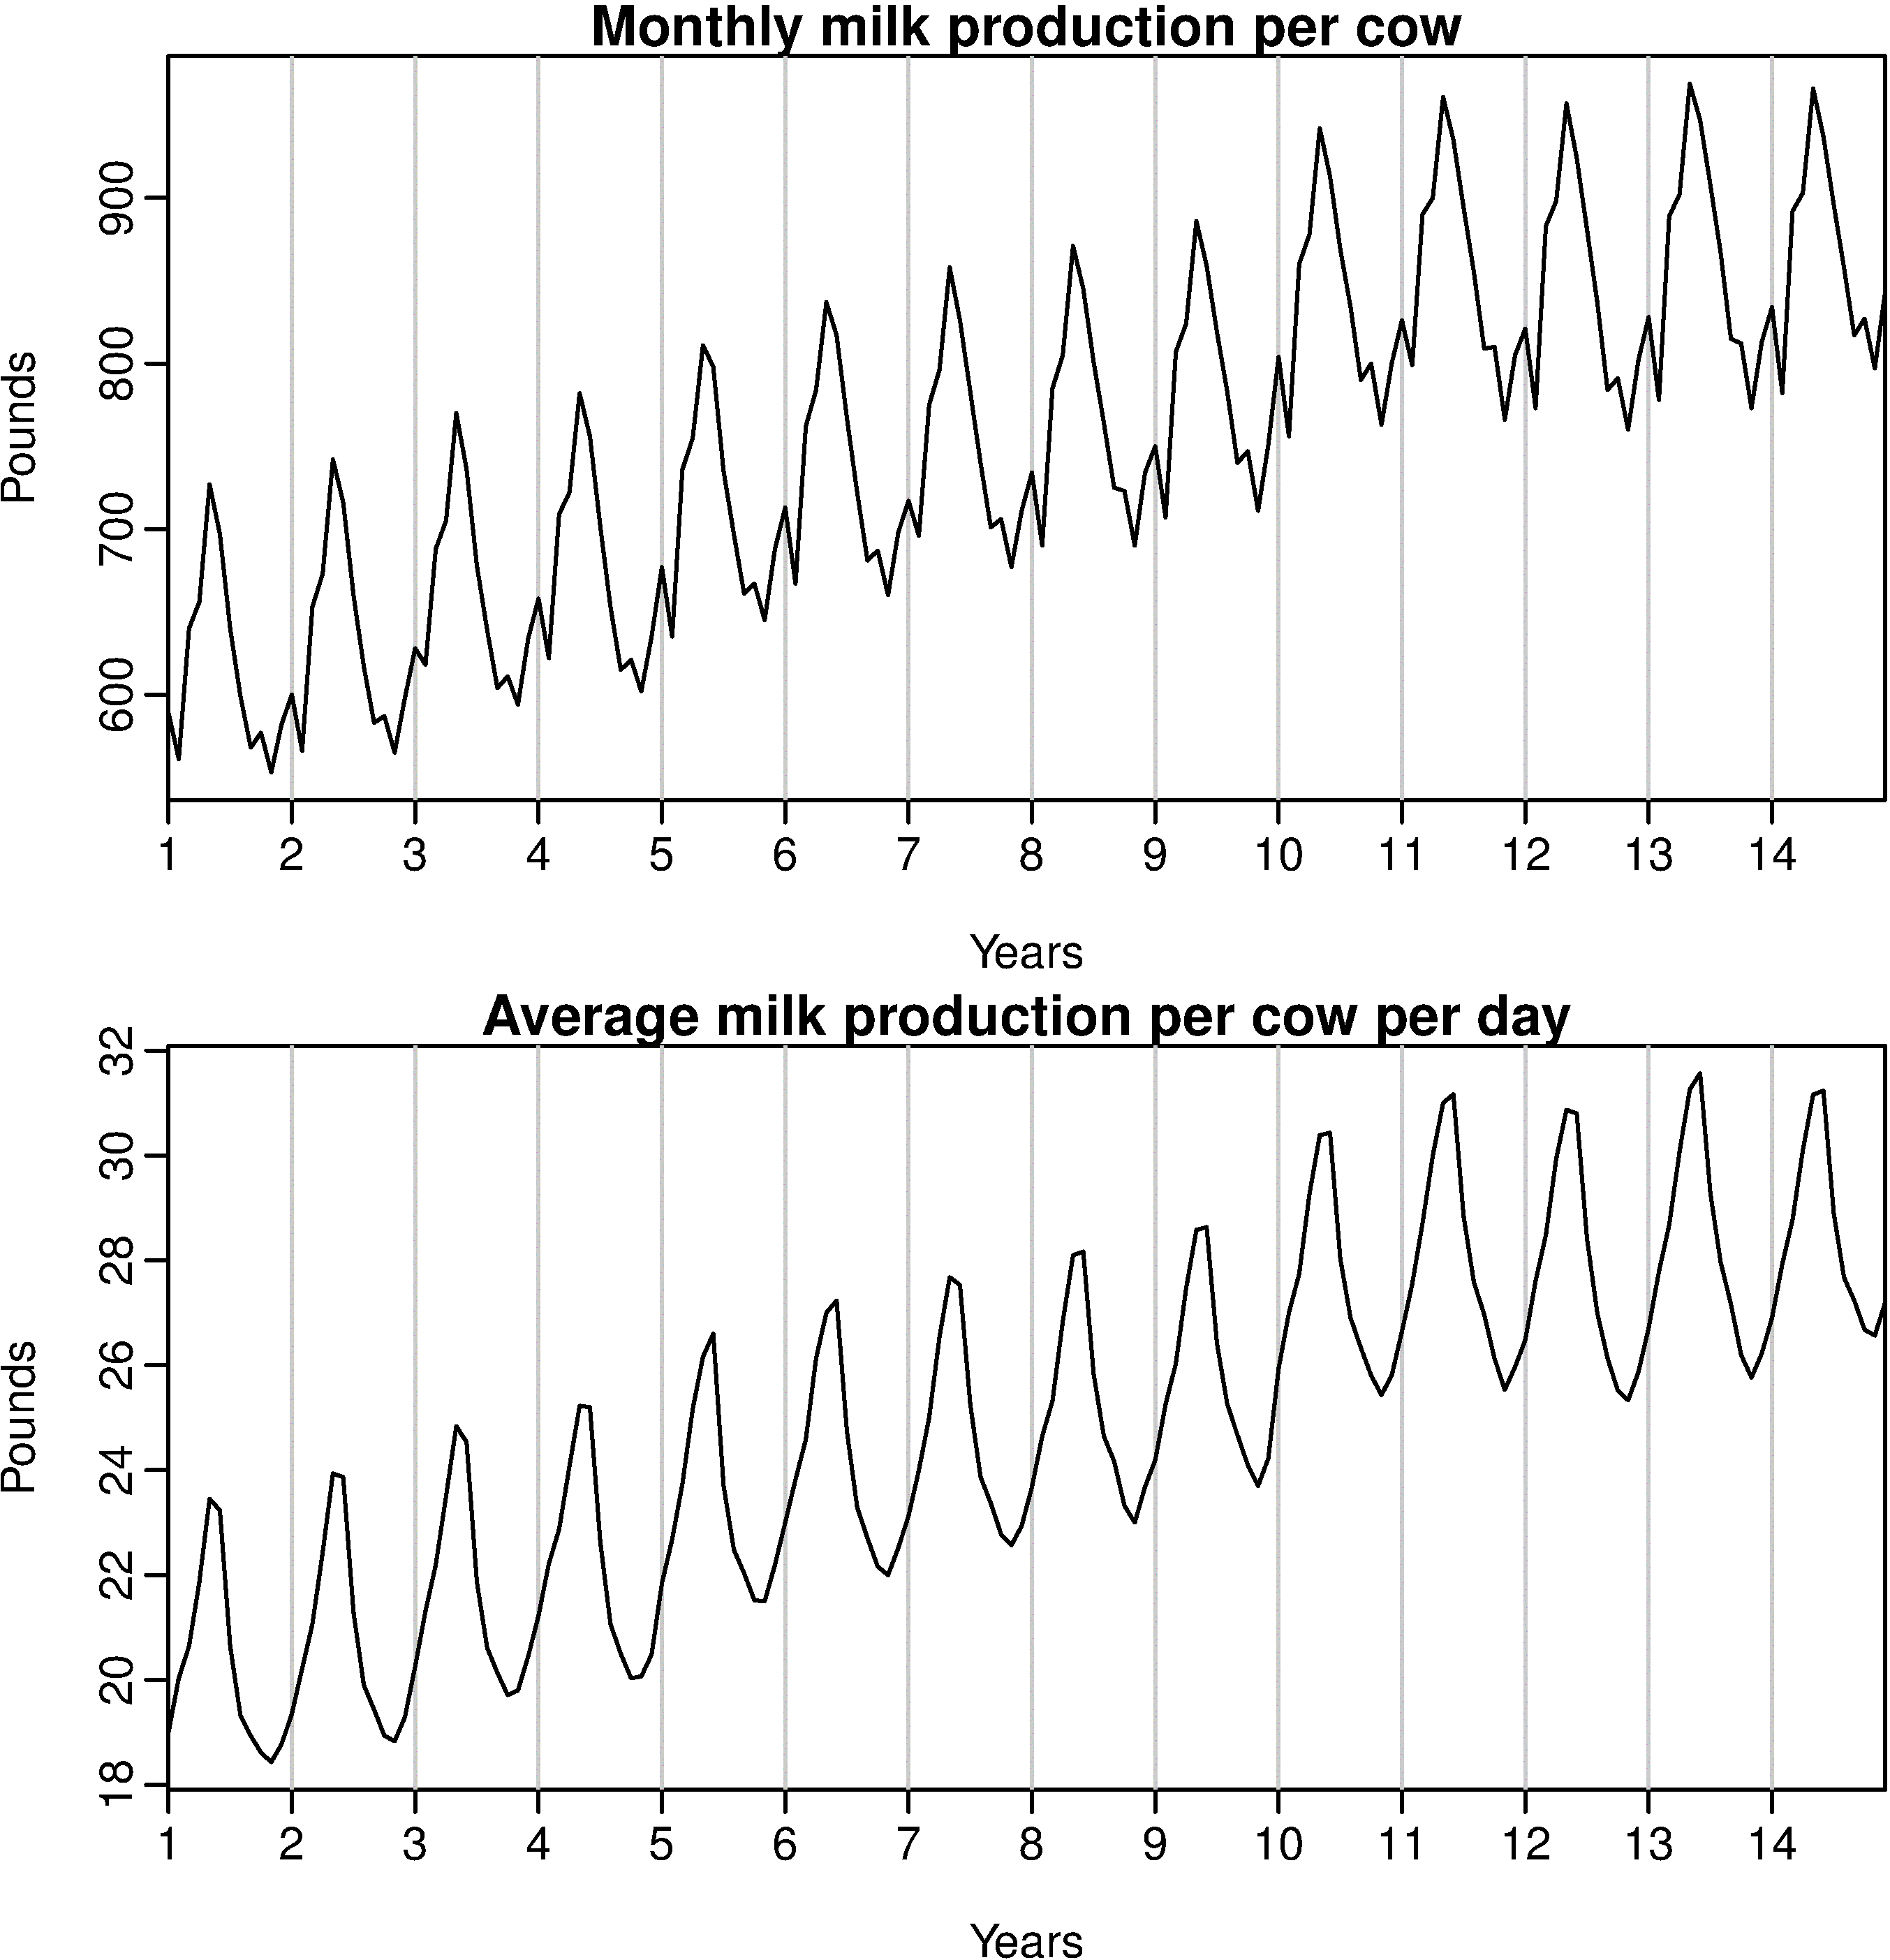
\includegraphics[height=0.6\textheight]{milk.png}
	\end{center}
\end{frame}

\subsection{Стационарность}
\begin{frame}{Стационарность}
	\only<1>{
%%%%%%%%%%%%%%%%%%%%%%%%%%%%%%%%%%%%%%%%%%%%%%%%%%%%%%%%%%%%%%%%%%%%%%%	
% Важное свойство временных рядов — это стационарность. Временной ряд  называется стационарным, если распределение его отсчётов в окне произвольной фиксированной ширины не зависит от положения этого окна, т.е. свойства ряда не зависят от времени.
% Из этого определения следует, что ряды, в которых присутствует тренд, являются нестационарными: в зависимости от расположения окна изменяется средний уровень ряда. Кроме того, нестационарны ряды с сезонностью: если ширина окна меньше сезонного периода, то распределение ряда будет разным в зависимости от положения окна. При этом интересно, что ряды, в которых есть непериодические циклы, не обязательно являются нестационарными, поскольку нельзя заранее предсказать положение максимумов и минимумов этого ряда.
%%%%%%%%%%%%%%%%%%%%%%%%%%%%%%%%%%%%%%%%%%%%%%%%%%%%%%%%%%%%%%%%%%%%%%%	
		Ряд $y_1,\dots,y_T$ \textbf{стационарен}, если $\forall s$ распределение $y_t,\dots,y_{t+s}$ не зависит от $t$, т.\,е. его свойства не зависят от времени.
		
		\bigskip
		
		Ряды с трендом или сезонностью нестационарны.
		
		\bigskip
		
		Ряды с непериодическими циклами стационарны, поскольку нельзя предсказать заранее, где будут находится максимумы и~минимумы.
	}
	
	\only<2>{
%%%%%%%%%%%%%%%%%%%%%%%%%%%%%%%%%%%%%%%%%%%%%%%%%%%%%%%%%%%%%%%%%%%%%%%	
% Как вы думаете, какие из этих рядов стационарны?
%%%%%%%%%%%%%%%%%%%%%%%%%%%%%%%%%%%%%%%%%%%%%%%%%%%%%%%%%%%%%%%%%%%%%%%	
		\begin{center}
			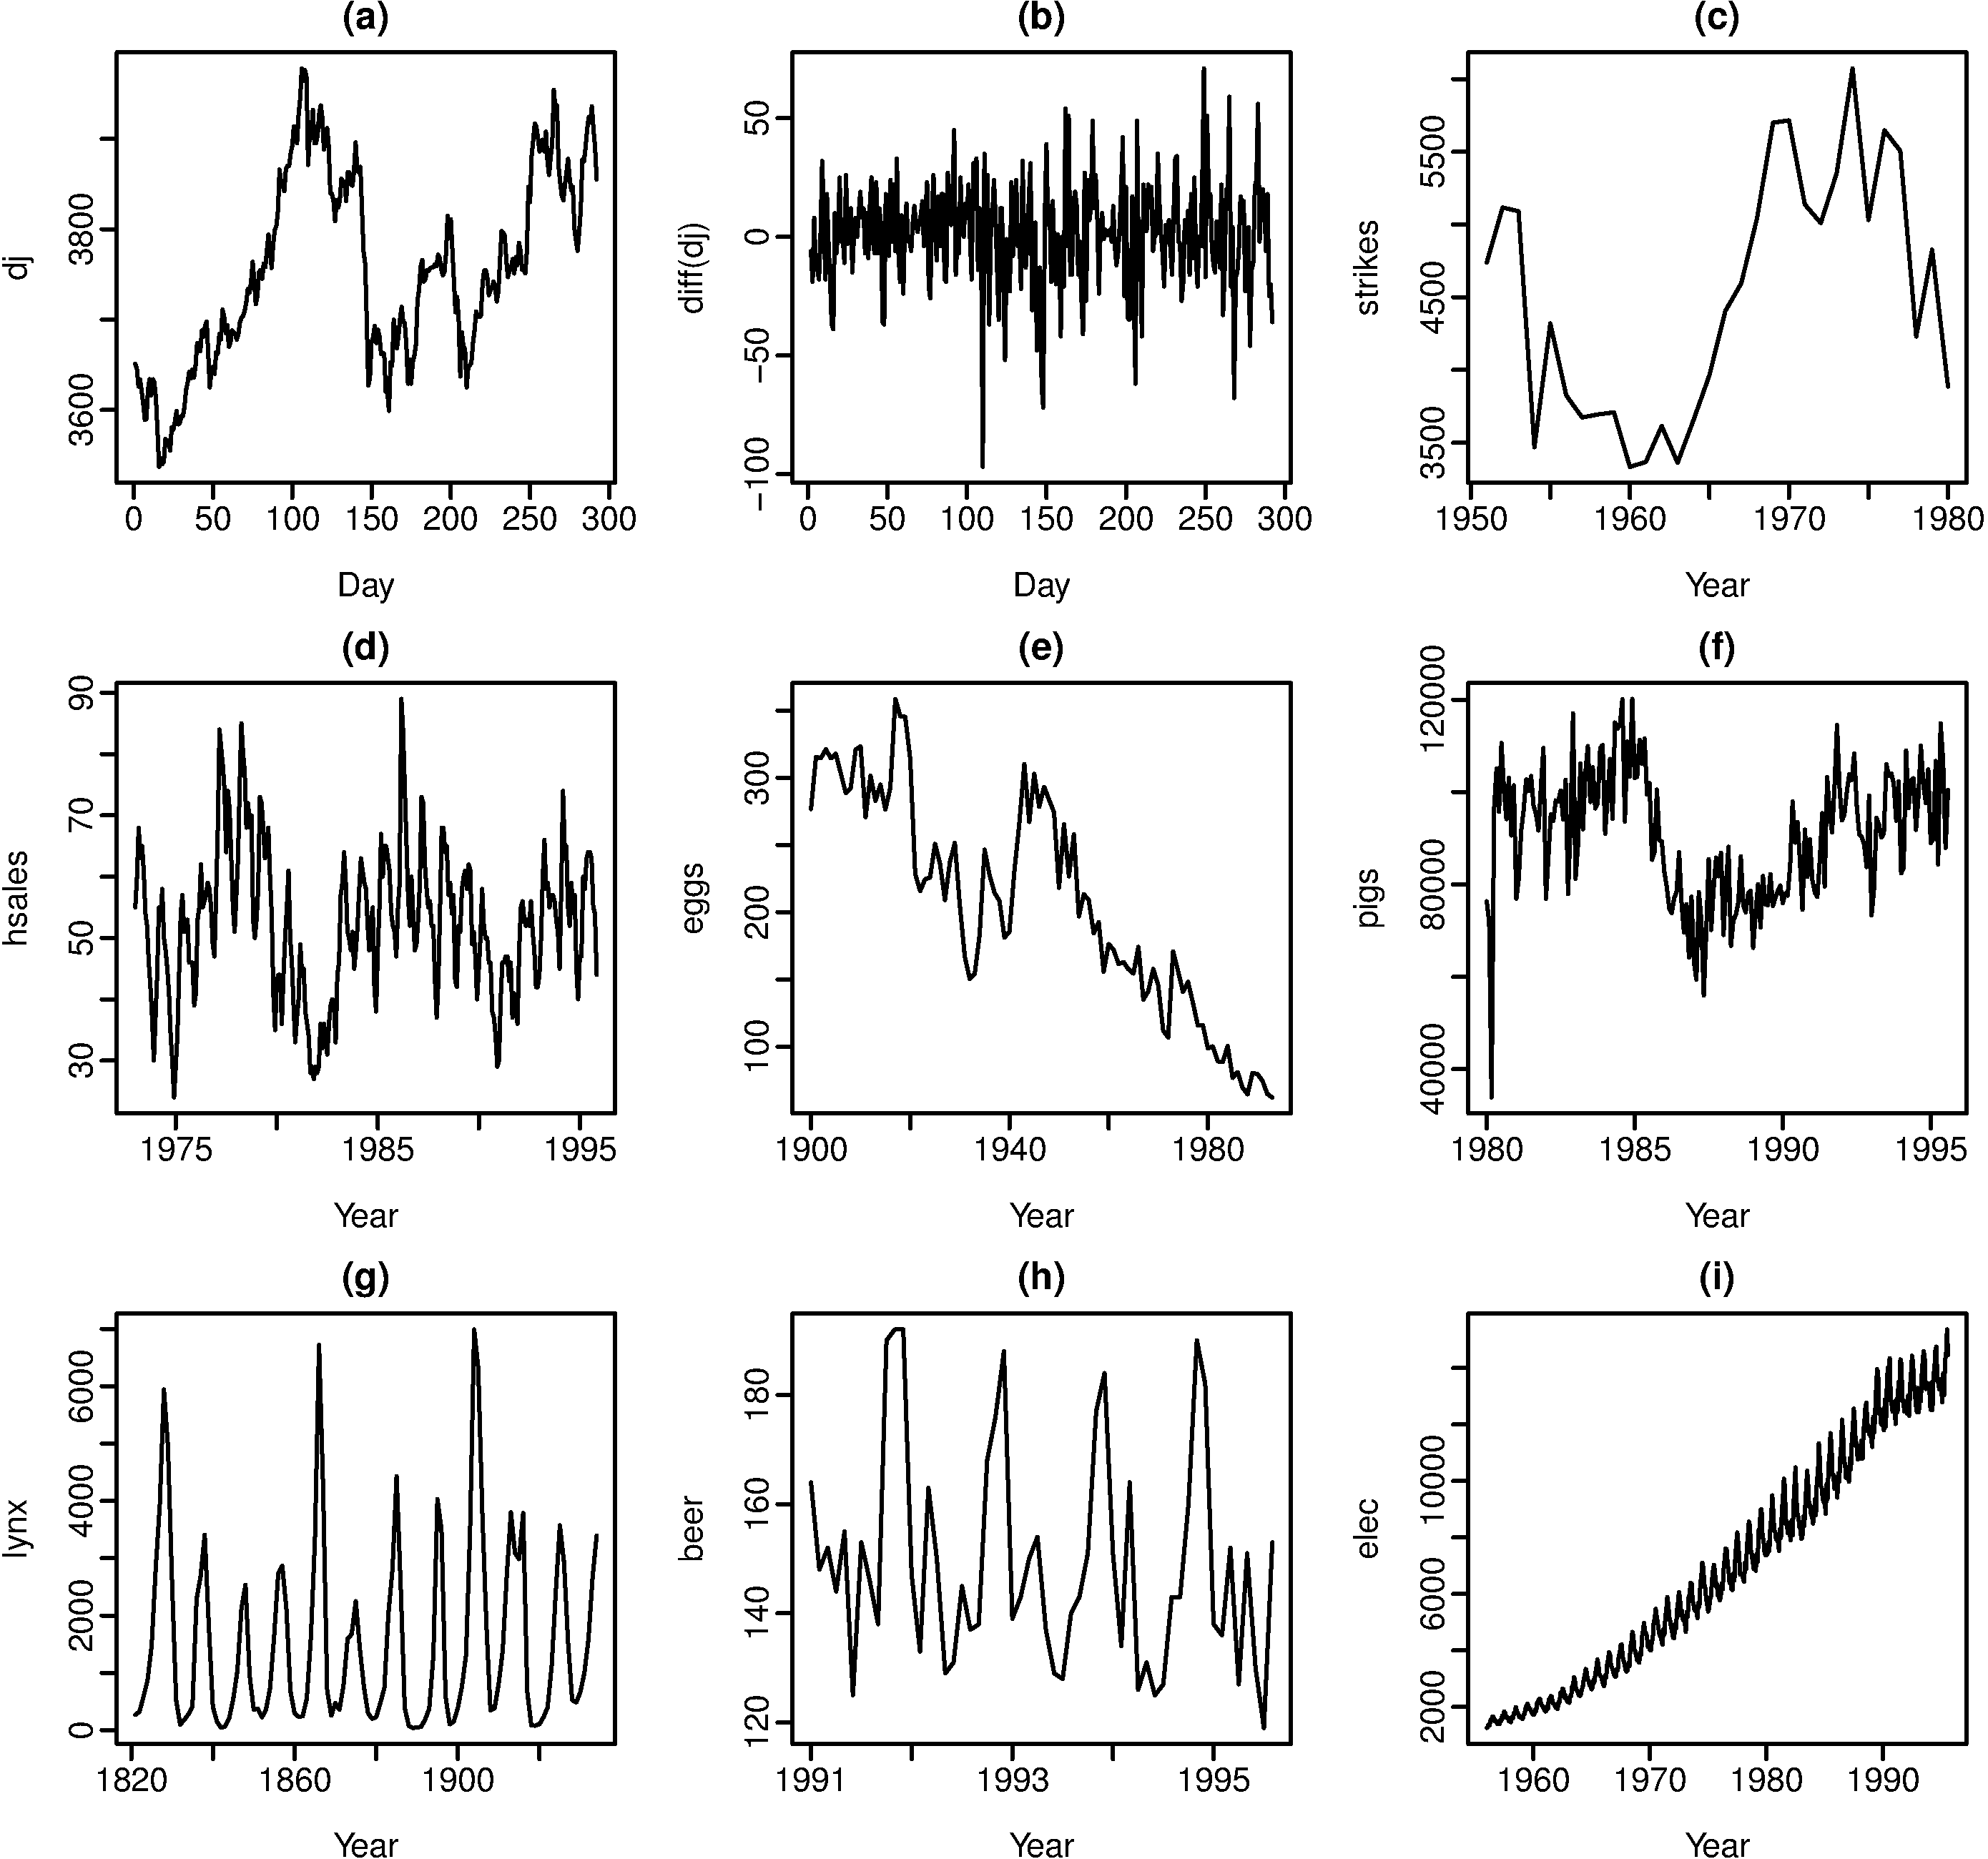
\includegraphics[height=0.7\textheight]{stationary.png}			
		\end{center}	
	}
	
	\only<3>{
		Нестационарны из-за сезонности:
		\begin{center}
			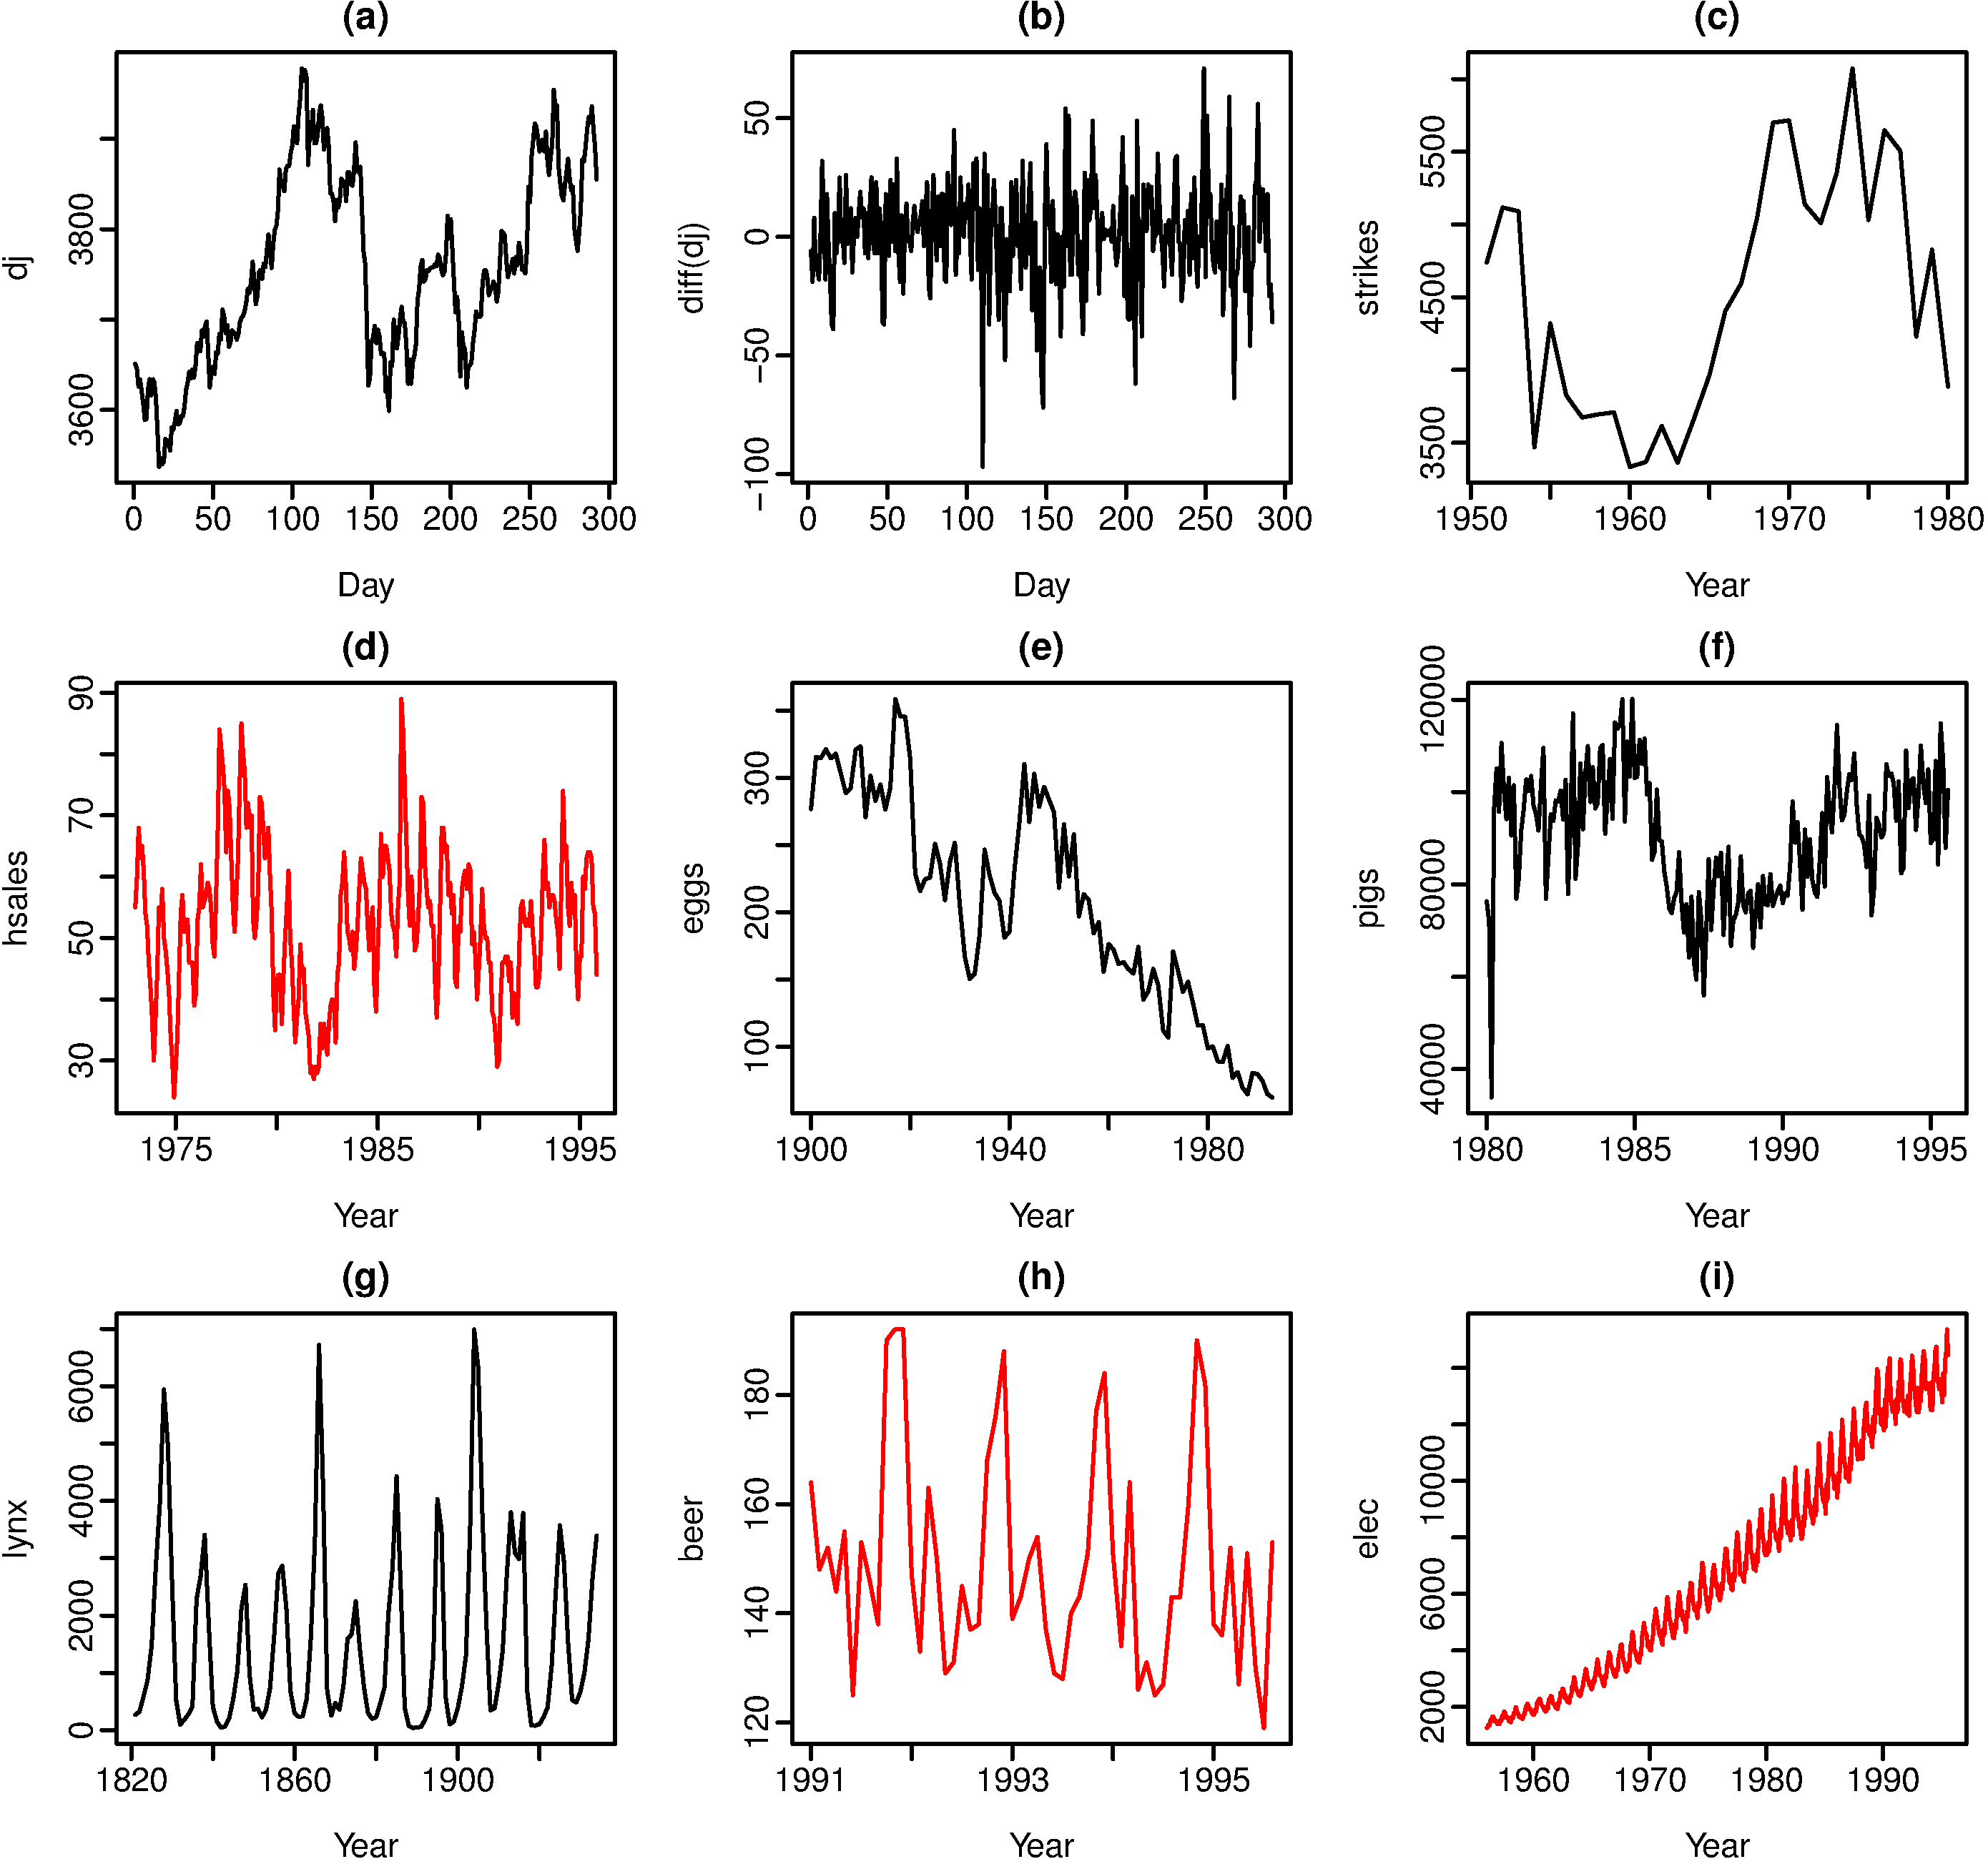
\includegraphics[height=0.7\textheight]{stationary1.png}			
		\end{center}	
	}	
	
	\only<4>{
		Нестационарны из-за тренда:
		\begin{center}
			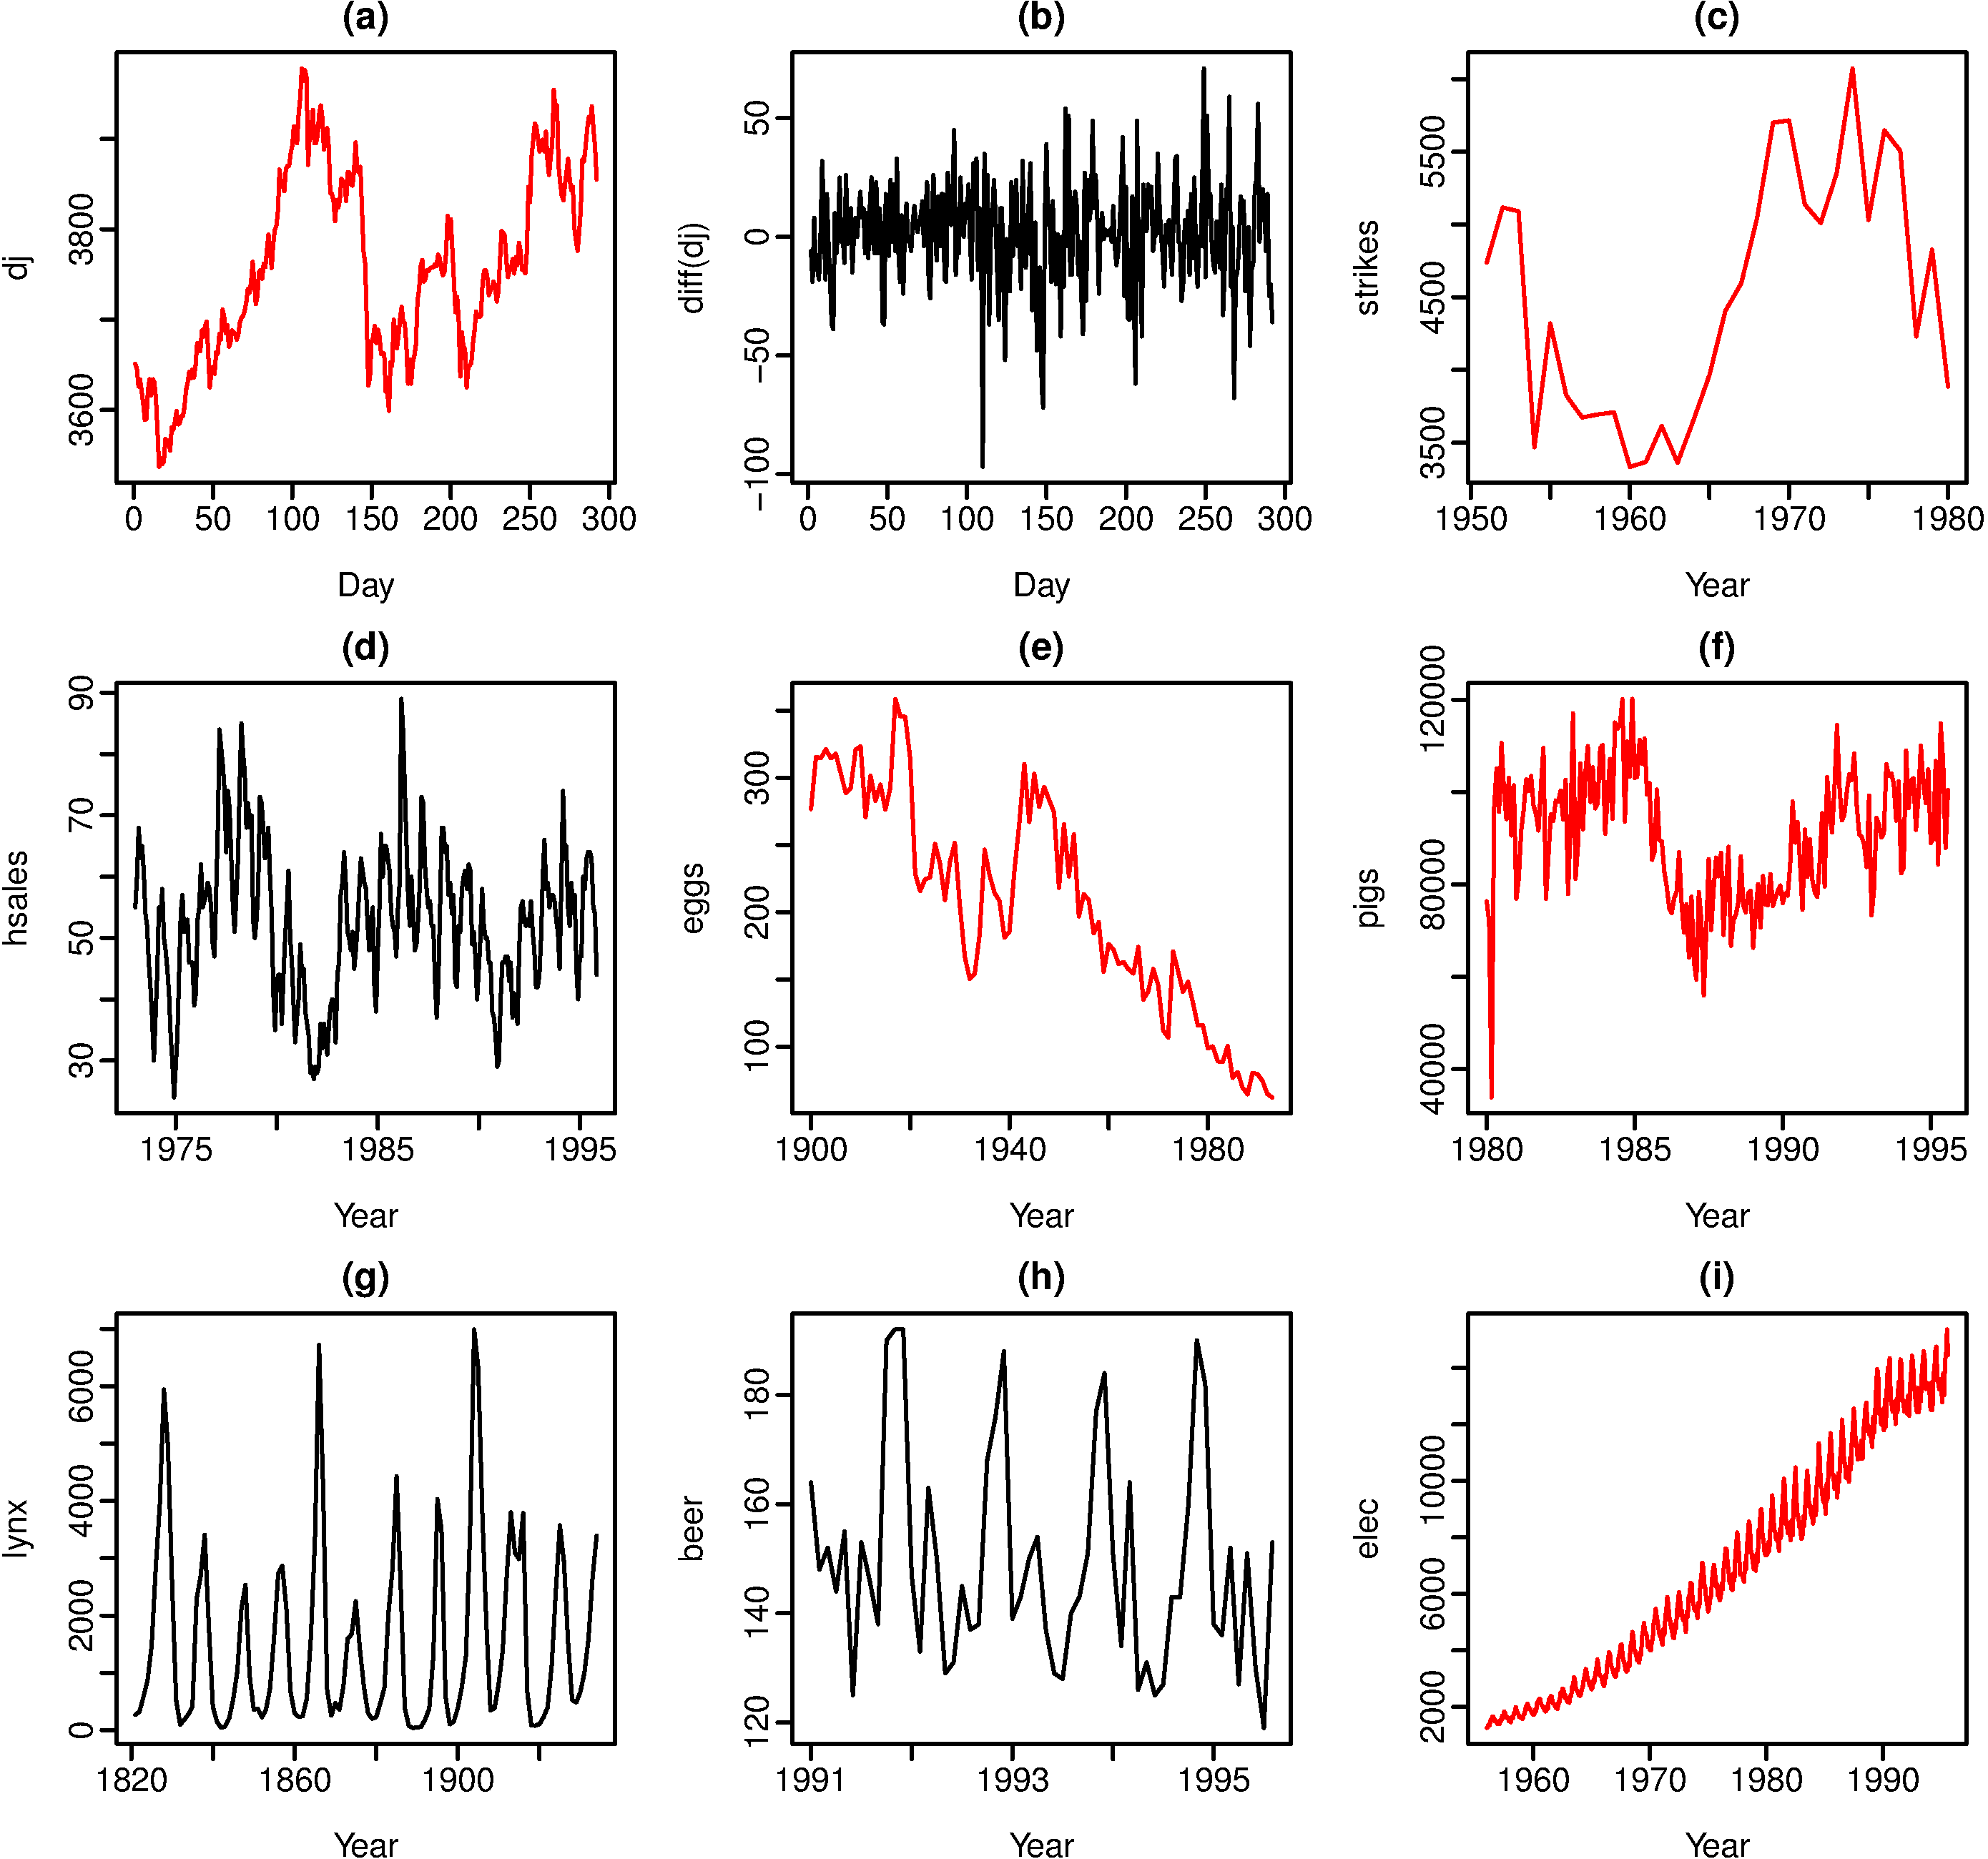
\includegraphics[height=0.7\textheight]{stationary2.png}			
		\end{center}	
	}		
	
	\only<5>{
		Нестационарны из-за меняющейся дисперсии:
		\begin{center}
			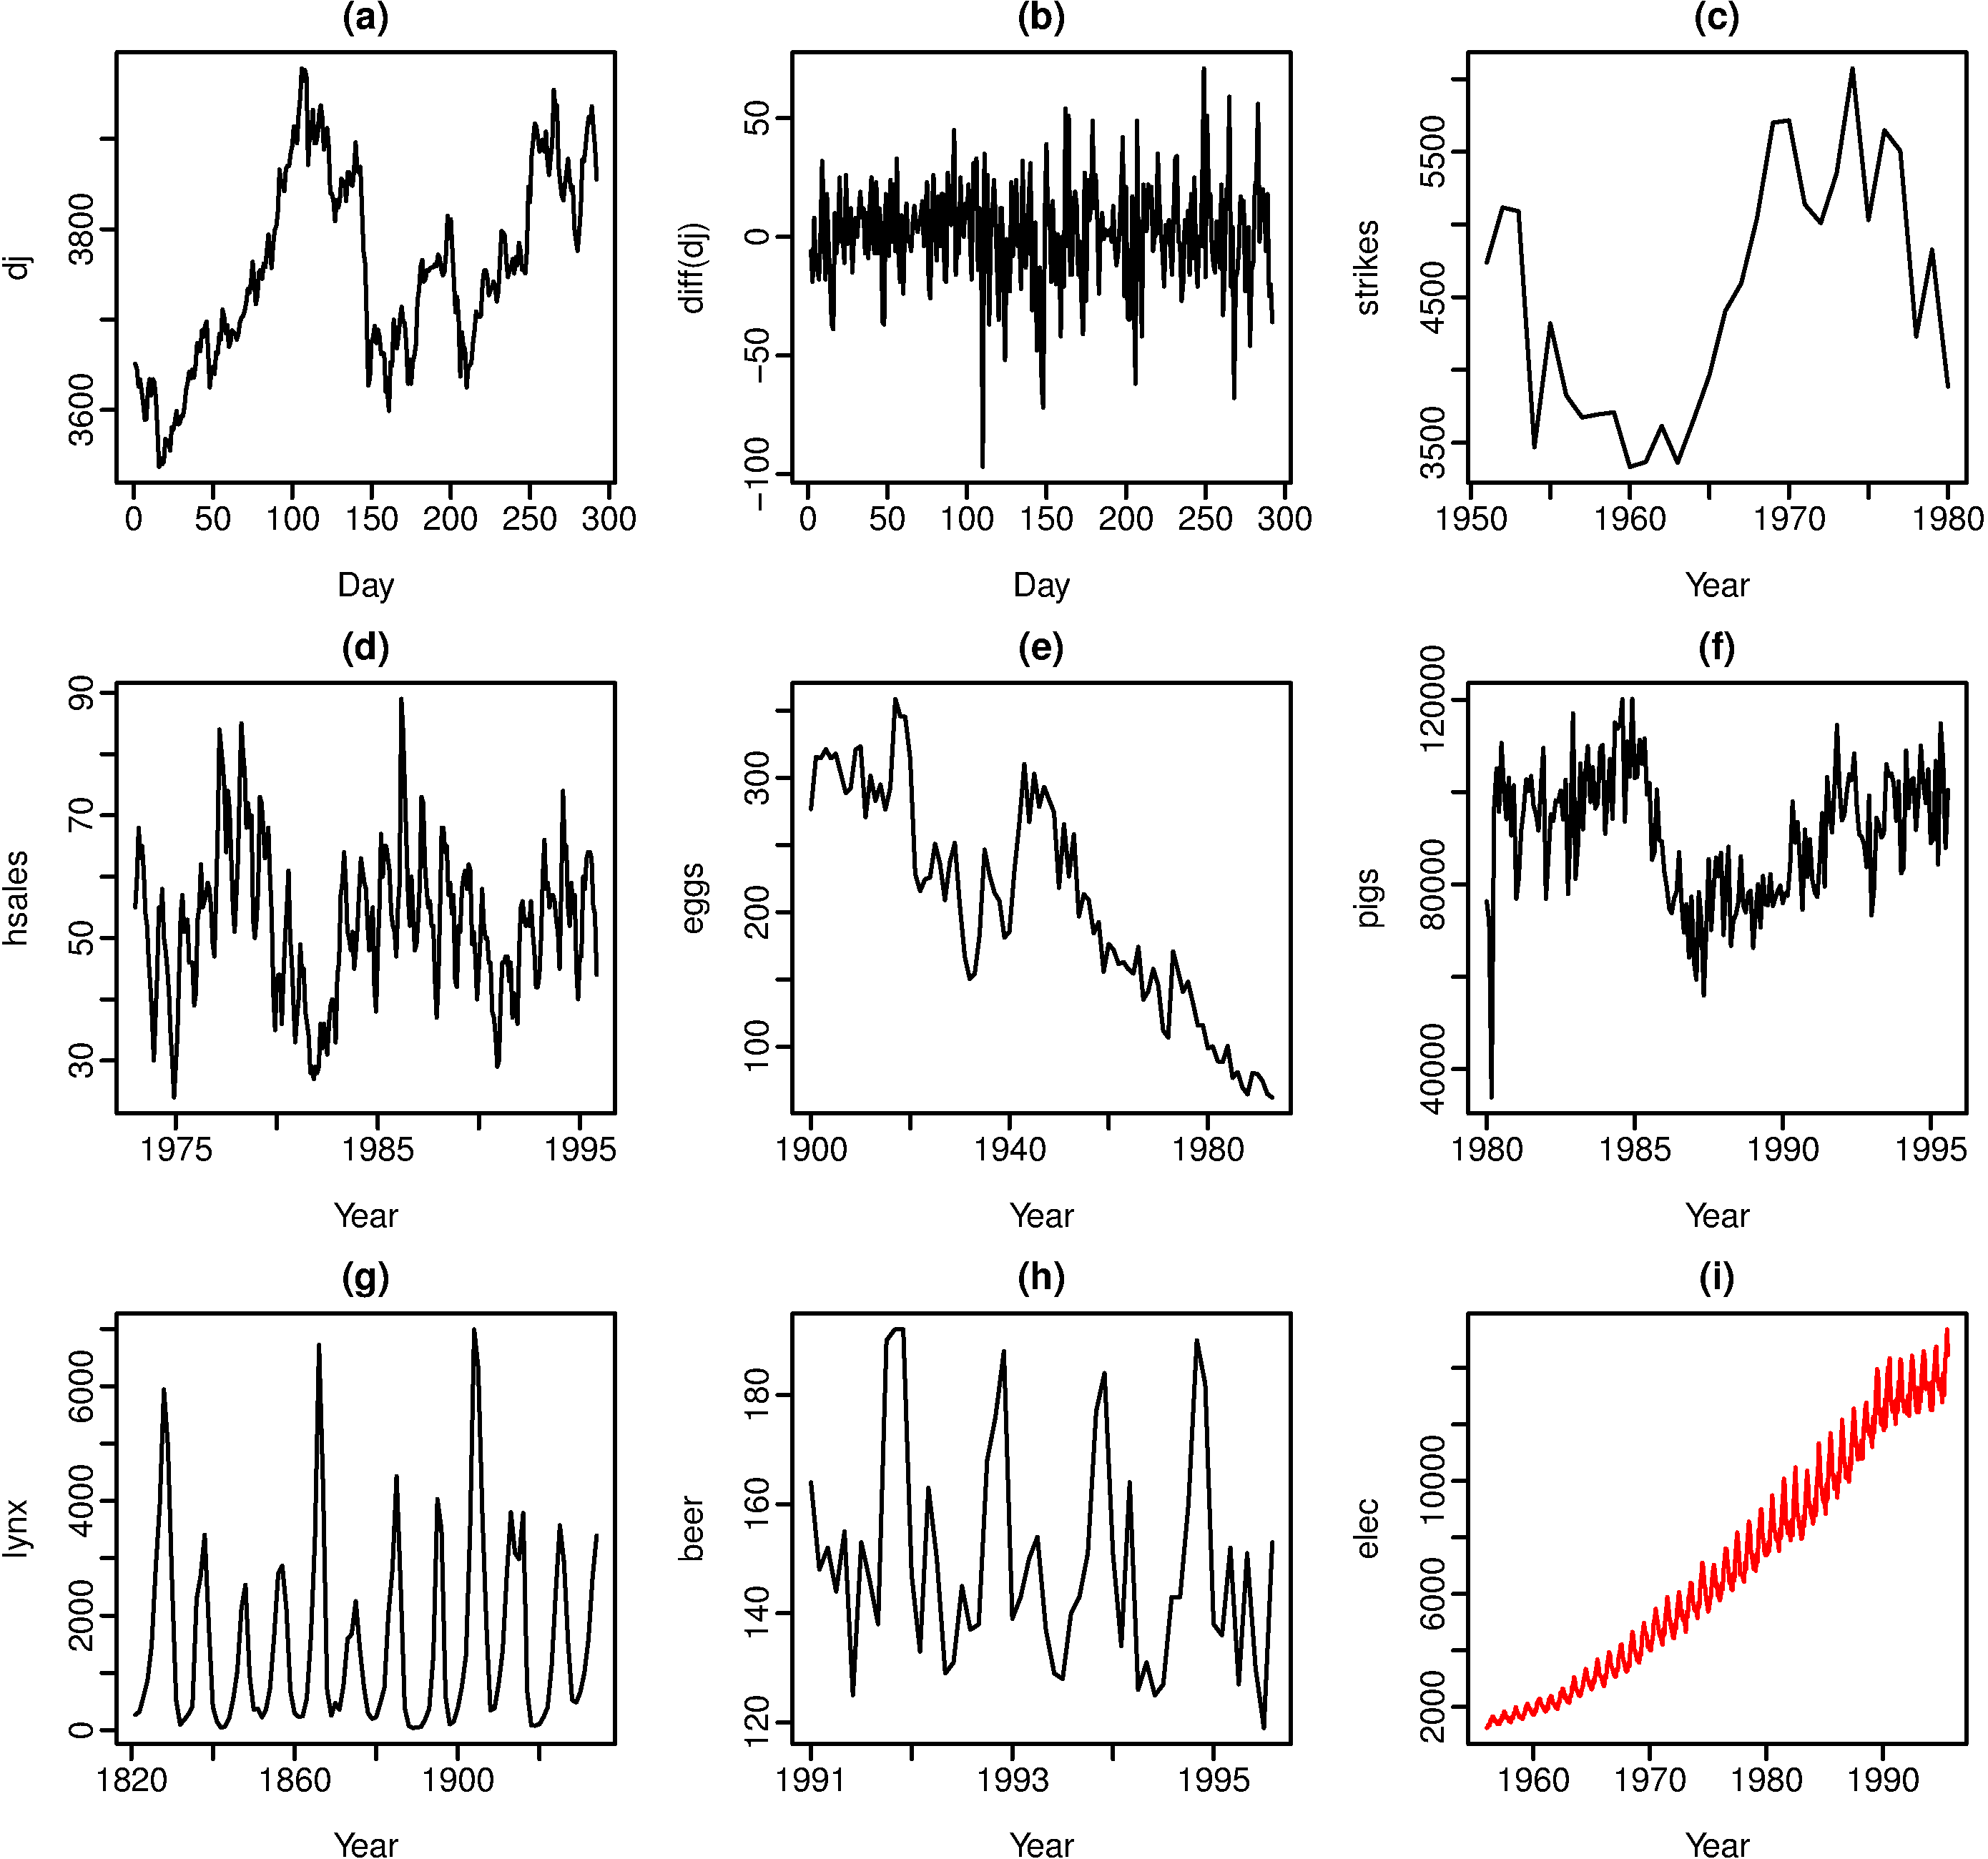
\includegraphics[height=0.7\textheight]{stationary3.png}			
		\end{center}	
	}
	
	\only<6>{
		Стационарны:
		\begin{center}
			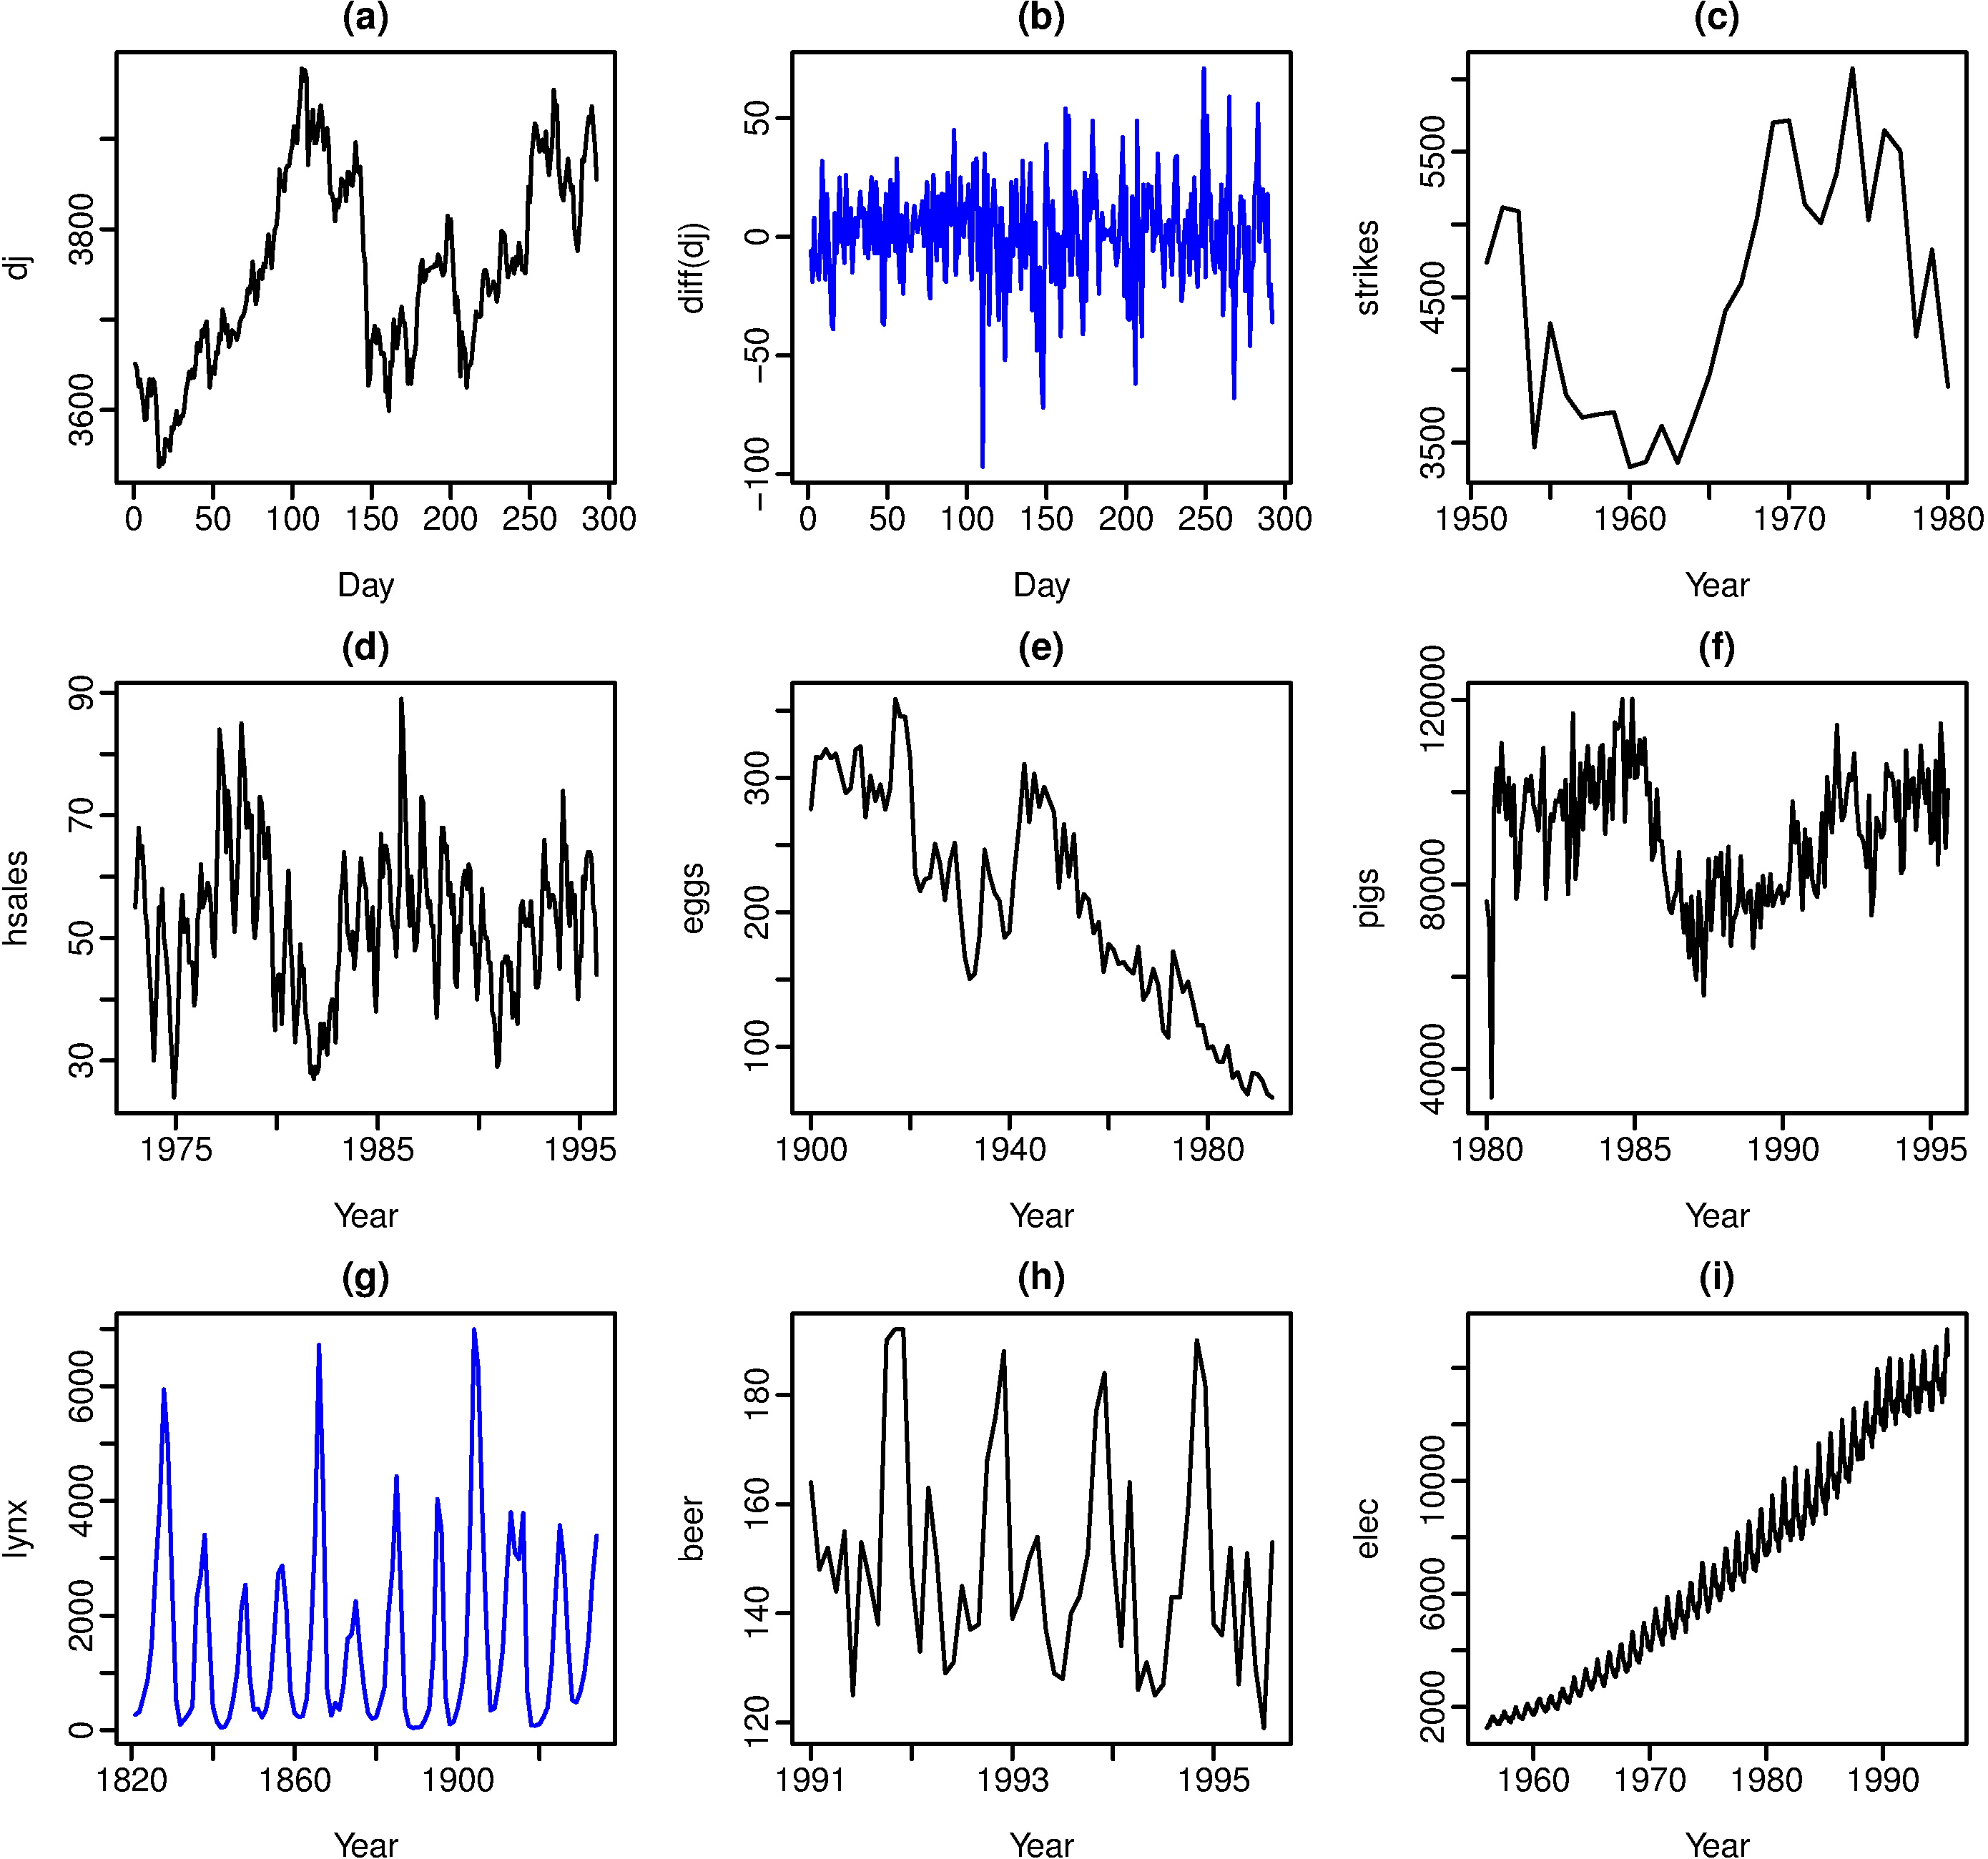
\includegraphics[height=0.7\textheight]{stationary4.png}
		\end{center}	
	}
\end{frame}


\begin{frame}{Критерий KPSS (Kwiatkowski-Philips-Schmidt-Shin)}
%%%%%%%%%%%%%%%%%%%%%%%%%%%%%%%%%%%%%%%%%%%%%%%%%%%%%%%%%%%%%%%%%%%%%%%			
% Формально гипотезу о стационарности можно проверить с помощью критерия KPSS. Статистика критерия выглядит достаточно сложно, не будем вдаваться в подробности. Вообще говоря, существует большое количество критериев для проверки гипотезы о стационарности, на практике можно использовать любой из них. Следите только, что именно для критерия является нулевой гипотезой - у некоторых критериев это стационарность, как у KPSS, у других, наоборот, её отсутствие.
%%%%%%%%%%%%%%%%%%%%%%%%%%%%%%%%%%%%%%%%%%%%%%%%%%%%%%%%%%%%%%%%%%%%%%%			
	\begin{center}
		\begin{tabular}{rl}
			ряд ошибок прогноза:            & $\varepsilon^T = \varepsilon_1,\dots,\varepsilon_T;$ \\
			нулевая гипотеза:               & $H_0\colon$ ряд $\varepsilon^T$ стационарен;\\
			альтернатива:                   & $H_1\colon$ ряд $\varepsilon^T$ описывается моделью \\
			& вида $\varepsilon_t = \alpha\varepsilon_{t-1};$ \\
			статистика:                     & $KPSS\left(\varepsilon^T\right) = \frac1{T^2} \sum\limits_{i=1}^T \left(\sum\limits_{t=1}^i \varepsilon_t\right)^2 \Big/ \lambda^2,$ \\
            &$\lambda^2$---оценка дисперсии ошибок;\\
			нулевое распределение:          & табличное.\\
		\end{tabular}
	\end{center}
	
	\bigskip
	
	Другие критерии для проверки стационарности: Дики"=Фуллера, Филлипса"=Перрона и их многочисленные модификации (см. Patterson K.  \textit{Unit root tests in time series, volume 1: key concepts and problems}. --- Palgrave Macmillan, 2011).	
\end{frame}


\subsection{Преобразования ряда}
\begin{frame}{Стабилизация дисперсии}
%%%%%%%%%%%%%%%%%%%%%%%%%%%%%%%%%%%%%%%%%%%%%%%%%%%%%%%%%%%%%%%%%%%%%%%	
% При работе с нестационарными временными рядами используется ряд стандартных трюков, чтобы сделать их стационарными. В случае, если во временном ряде монотонно по времени изменяется дисперсия, применяется специальное преобразование, стабилизирующее дисперсию. Очень часто в качестве такого преобразования выступает логарифмирование. Результат стабилизации дисперсии для ряда производства электричества в Австралии показан на рисунке 1.15. Видно, что после логарифмирования размах колебаний в начале и конце ряда становится очень похожим, и дисперсия примерно стабилизируется.
%%%%%%%%%%%%%%%%%%%%%%%%%%%%%%%%%%%%%%%%%%%%%%%%%%%%%%%%%%%%%%%%%%%%%%%	
	Для рядов с монотонно меняющейся дисперсией можно использовать стабилизирующие преобразования.
	
	
	\bigskip
	
	Часто используют логарифмирование:
	
	\bigskip
	
	\begin{center}
		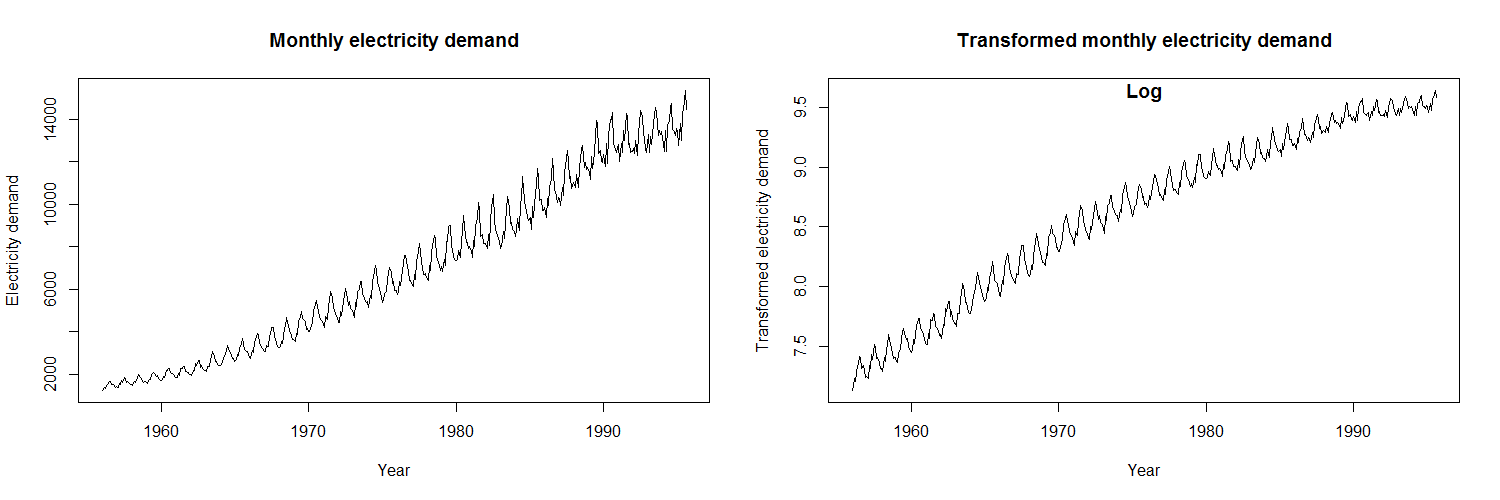
\includegraphics[width=0.8\textwidth]{logtrans.png}
	\end{center}		
\end{frame}

\begin{frame}{Преобразования Бокса-Кокса}	
	\only<1>{
%%%%%%%%%%%%%%%%%%%%%%%%%%%%%%%%%%%%%%%%%%%%%%%%%%%%%%%%%%%%%%%%%%%%%%%	
% Логарифмирование принадлежит к семейству преобразований Бокса-Кокса. Это параметрическое семейство функций, в котором параметр  определяет, как именно будет преобразован ряд: лямбда = 0 — это логарифмирование, лямбда = 1 — тождественное преобразование ряда, а при других значениях лямбда — степенное преобразование. Значение параметра можно подбирать так, чтобы дисперсия была как можно более стабильной во времени. Так, для ряда по данным производства электричества в Австралии оптимальное значение  = 0:27, при этом дисперсия немного более стабильна, чем при логарифмировании.
%%%%%%%%%%%%%%%%%%%%%%%%%%%%%%%%%%%%%%%%%%%%%%%%%%%%%%%%%%%%%%%%%%%%%%%	
		Параметрическое семейство стабилизирующих дисперсию преобразований:	
		$$
		y'_t=\begin{cases}
		\ln y_t, & \lambda=0, \\
		\left(y_t^\lambda-1\right)/\lambda, & \lambda\neq 0.
		\end{cases}
		$$	
		
		\bigskip
		
		Параметр $\lambda$ выбирается так, чтобы минимизировать дисперсию или максимизировать правдоподобие модели.
		
		\bigskip
		
		\begin{center}
			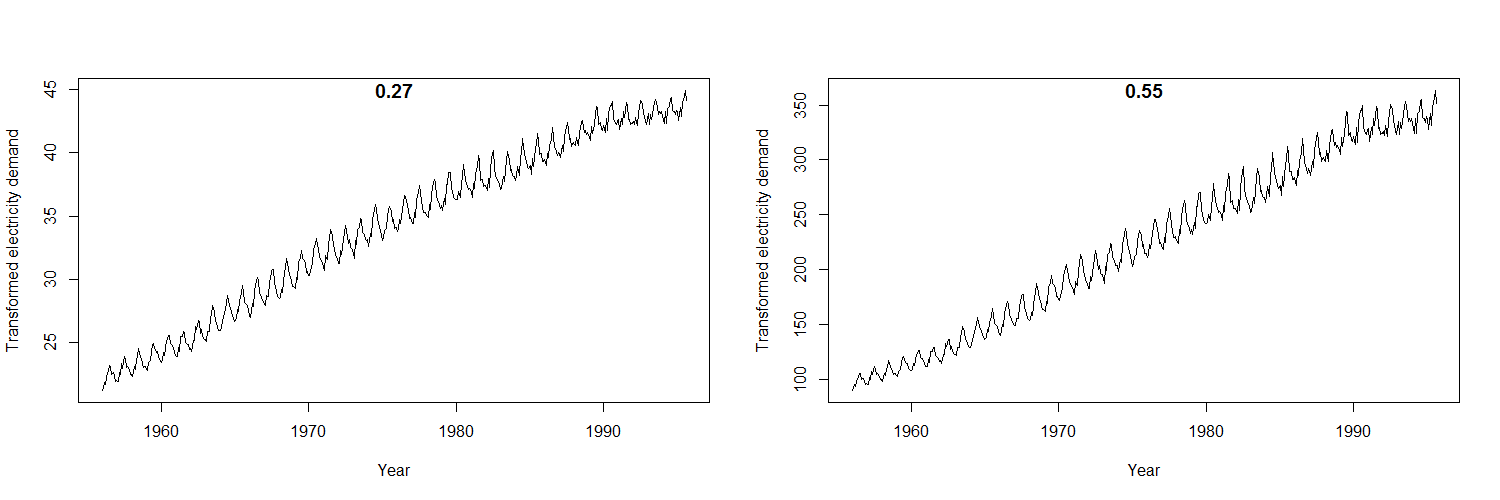
\includegraphics[width=0.8\textwidth]{boxcox.png}
		\end{center}
	}
	
	\only<2>{
		После построения прогноза для трансформированного ряда его нужно преобразовать в прогноз исходного:
		$$
		\hat{y}_t=\begin{cases}
		\exp\left(\hat{y}'_t\right), & \lambda=0, \\
		\left(\lambda\hat{y}'_t+1\right)^{1/\lambda}, & \lambda\neq 0.
		\end{cases}
		$$			
		
		\bigskip
		
		\begin{itemize}
			\item если некоторые $y_t\leq0$, преобразования Бокса-Кокса невозможны (нужно прибавить к ряду константу)
			\item часто оказывается, что преобразование вообще не нужно
			\item можно округлять значение $\lambda,$ чтобы упростить интерпретацию
			\item как правило, стабилизирующее преобразование слабо влияет на~прогноз и сильно~--- на~предсказательный интервал
		\end{itemize}
	}
\end{frame}

\begin{frame}{Дифференцирование}
	\only<1>{
%%%%%%%%%%%%%%%%%%%%%%%%%%%%%%%%%%%%%%%%%%%%%%%%%%%%%%%%%%%%%%%%%%%%%%%	
% Ещё один важный трюк, который позволяет сделать ряд стационарным, — это дифференцирование, переход к попарным разностям соседних значений. Для нестационарного ряда часто оказывается, что получаемый после дифференцирования ряд является стационарным. Такая операция позволяет стабилизировать среднее значение ряда и избавиться от тренда, а иногда даже от сезонности. Кроме того, дифференцирование можно применять неоднократно: от ряда первых разностей, продифференцировав его, можно прийти к ряду вторых разностей, и т. д. Длина ряда при этом каждый раз будет немного сокращаться, но при этом он будет стационарным.
%%%%%%%%%%%%%%%%%%%%%%%%%%%%%%%%%%%%%%%%%%%%%%%%%%%%%%%%%%%%%%%%%%%%%%%	
		\textbf{Дифференцирование ряда}~--- переход к попарным разностям его соседних значений:
		$$y_1,\dots,y_T \;\longrightarrow \;y'_2,\dots,y'_{T}, $$
		$$y'_t = y_t - y_{t-1}.$$
		
		Дифференцированием можно стабилизировать среднее значение ряда и~избавиться от тренда и сезонности.
		
		\bigskip
		
		Может применяться неоднократное дифференцирование; например, для второго порядка:
		$$y_1,\dots,y_T \longrightarrow y'_2,\dots,y'_{T} \longrightarrow y''_3,\dots,y''_{T},$$	
		$$y''_t = y'_t-y'_{t-1} = y_t - 2y_{t-1} + y_{t-2}.$$		
	}
	
	\only<2>{
		\begin{center}
			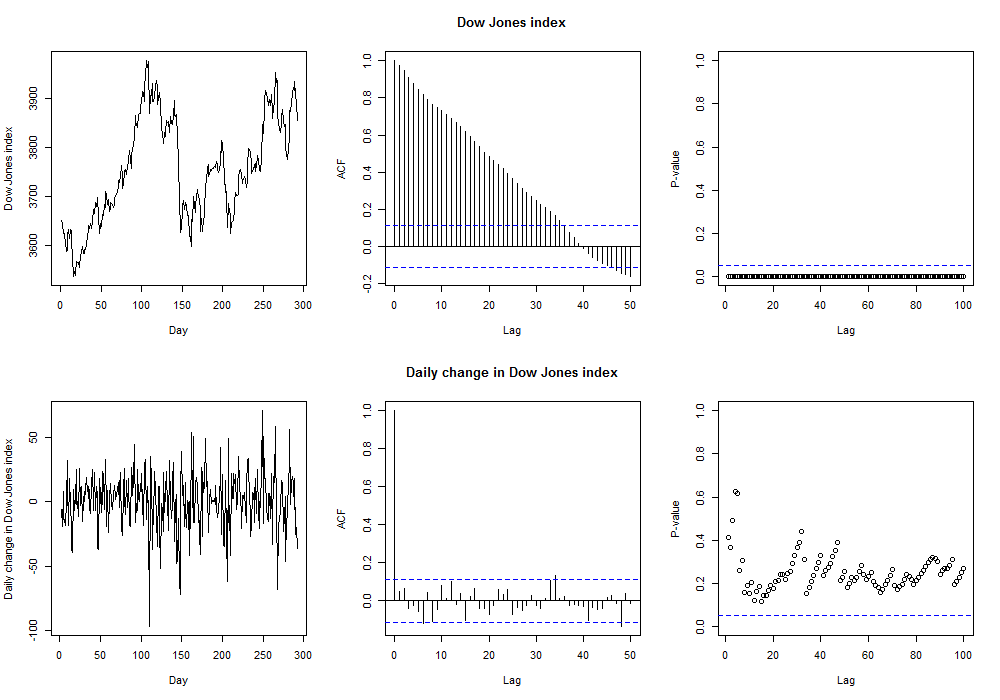
\includegraphics[height=0.8\textheight]{diff1.png}
		\end{center}	
		Критерий KPSS: для исходного ряда $p<0.01$, для ряда первых разностей~--- $p>0.1.$
	}
\end{frame}

\begin{frame}{Сезонное дифференцирование}
	\only<1>{
		\textbf{Сезонное дифференцирование ряда}~--- переход к попарным разностям его значений в соседних сезонах:
		$$y_1,\dots,y_T \;\longrightarrow \;y'_{s+1},\dots,y'_{T}, $$
		$$y'_t = y_t - y_{t-s}.$$	
	}
	
	\only<2>{

    	\begin{center}
    		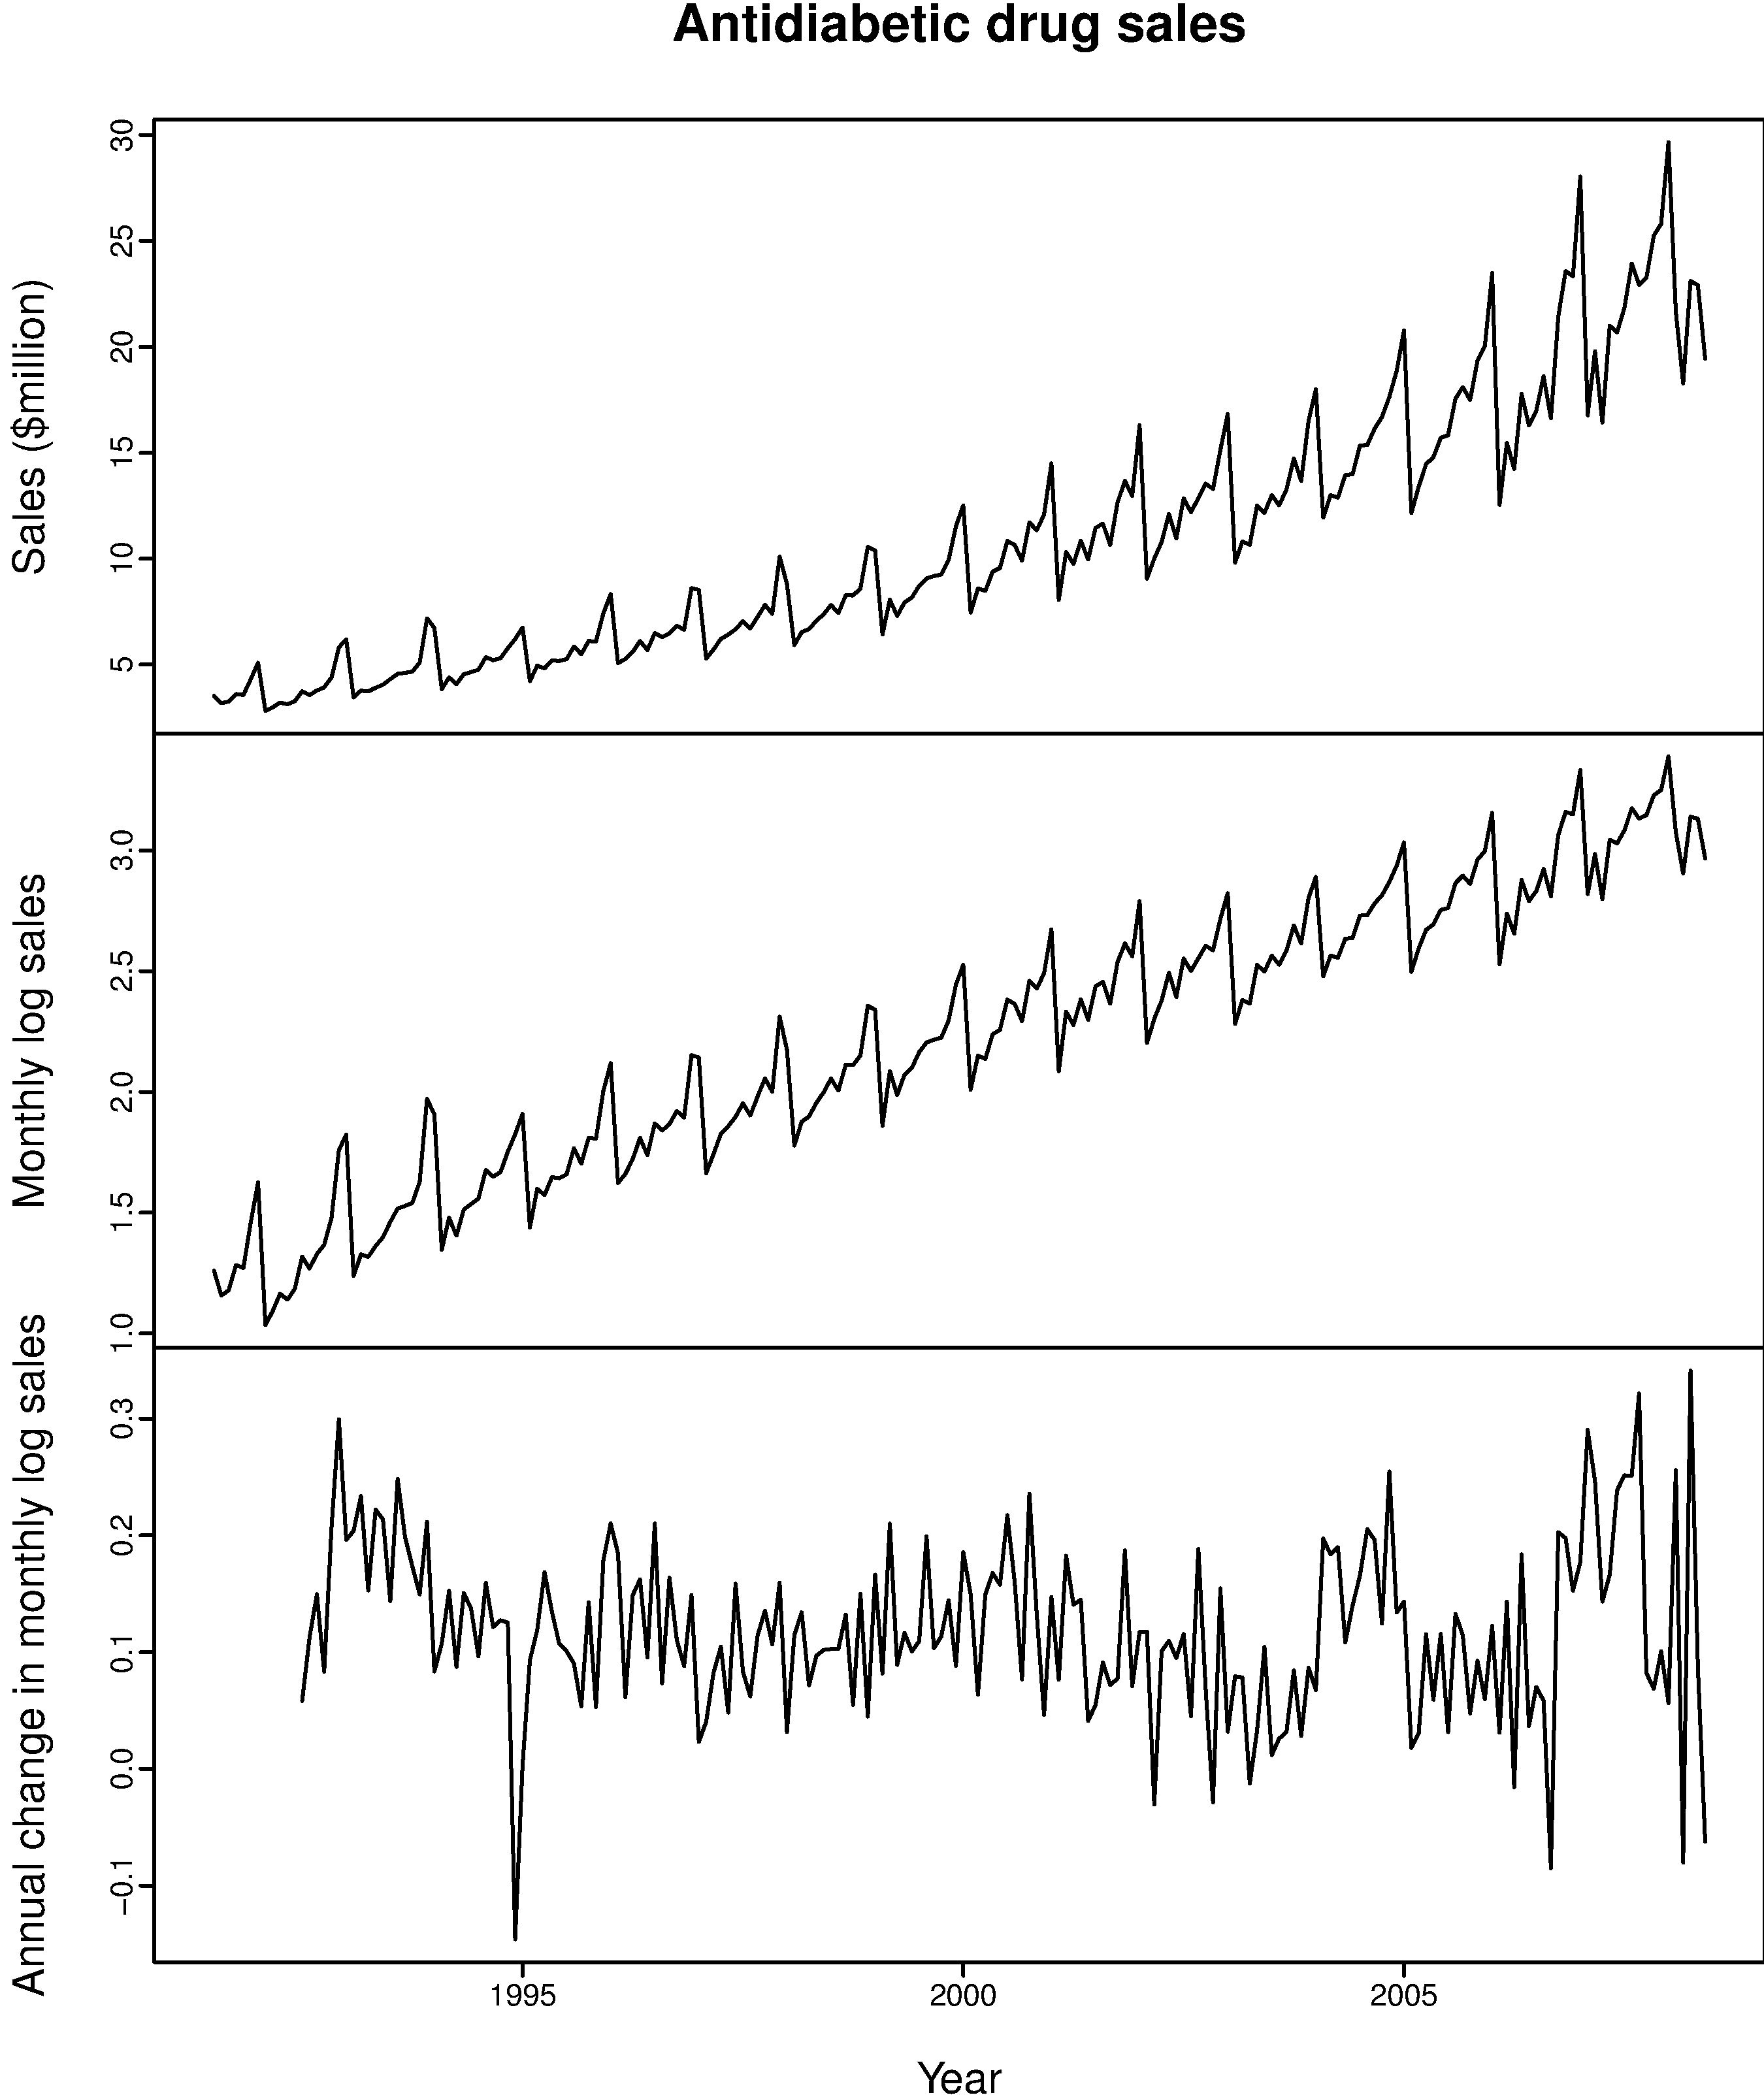
\includegraphics[height=0.7\textheight]{diffa10.png}
    	\end{center}
  
		
        Критерий~KPSS: для исходного ряда ${p<0.01},$ для логарифмированного~--- ${p<0.01},$ после сезонного дифференцирования~--- ${p>0.1}.$
	}
\end{frame}

\begin{frame}{Комбинированное дифференцирование}
	\only<1>{
		Сезонное и обычное дифференцирование может применяться к одному ряду в любом порядке.
		
		\bigskip
		
		Если ряд имеет выраженный сезонный профиль, рекомендуется начинать с сезонного дифференцирования~--- после него ряд уже может оказаться стационарным.
	}
	
	\only<2>{

    	\begin{center}
    		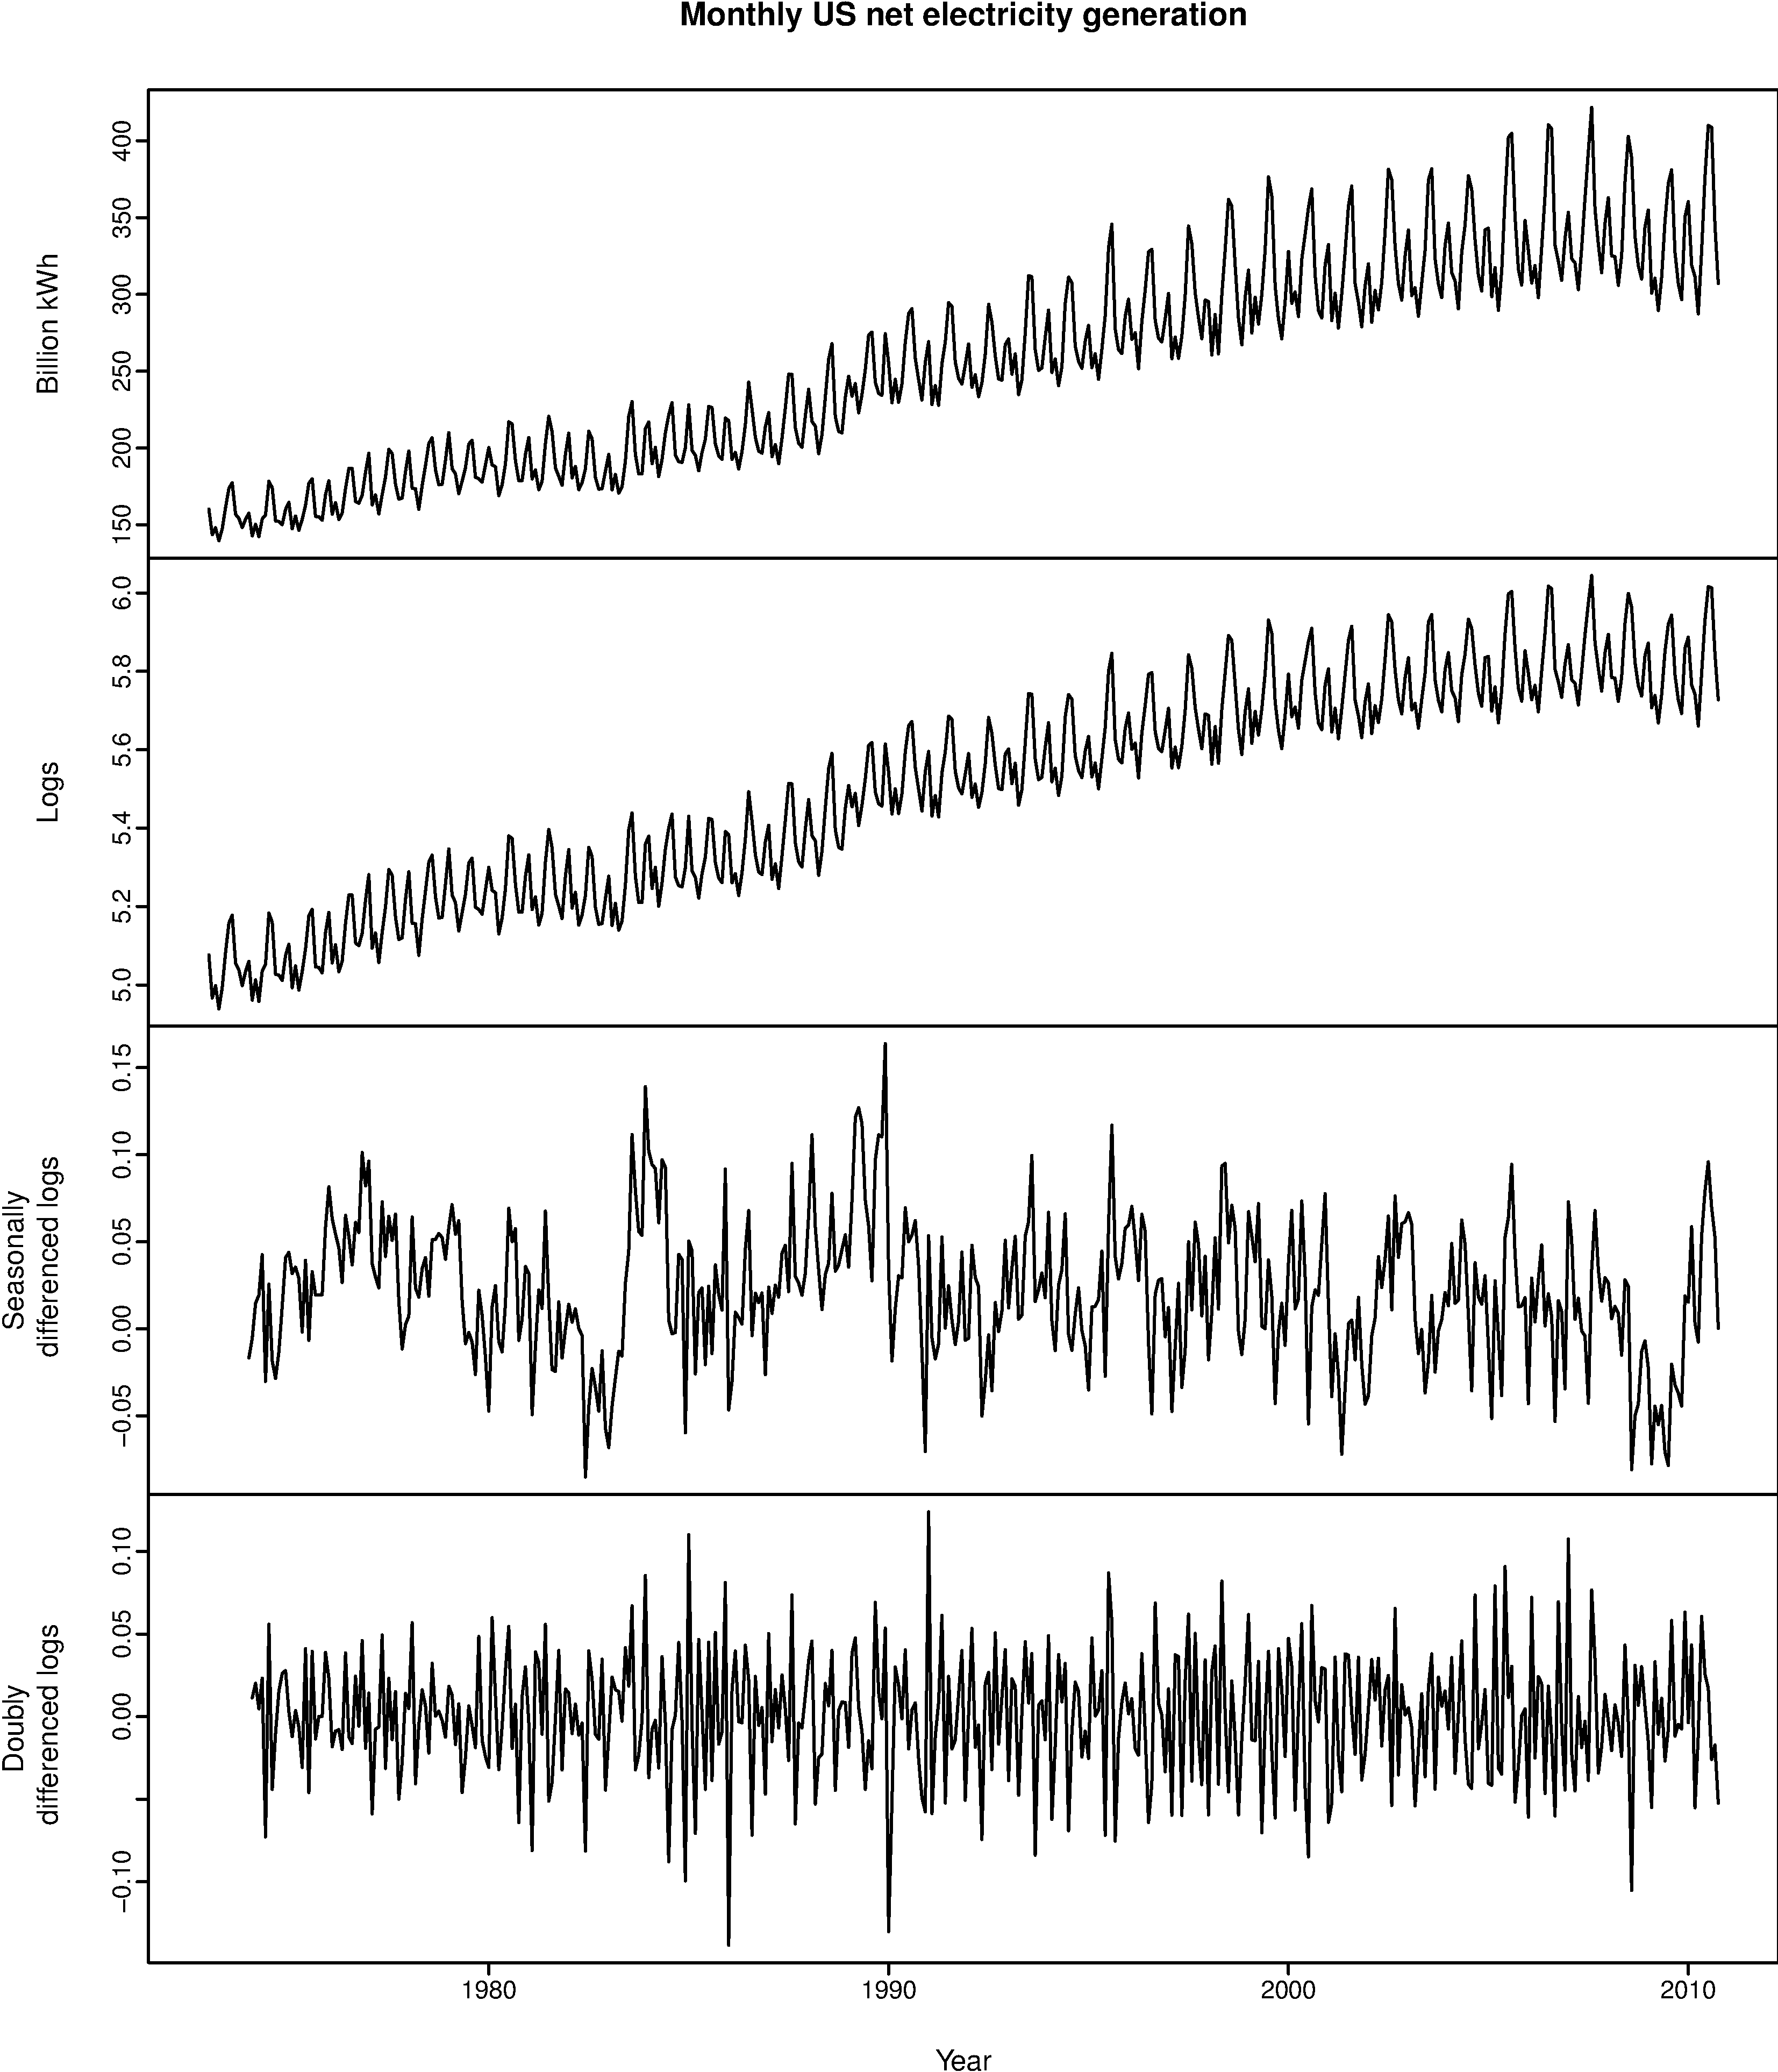
\includegraphics[height=0.6\textheight]{diffusnetelec.png}
    	\end{center}
  
        Критерий KPSS: для исходного ряда ${p<0.01},$ для логарифмированного~--- ${p<0.01},$ после сезонного дифференцирования~--- ${p=0.0355},$ после ещё одного дифференцирования~--- ${p>0.1}.$
	}
\end{frame}

\subsection{Анализ остатков}
\begin{frame}{Оcтатки}
%%%%%%%%%%%%%%%%%%%%%%%%%%%%%%%%%%%%%%%%%%%%%%%%%%%%%%%%%%%%%%%%%%%%%%%	
% Анализ остатков — это техника, которая помогает понять, есть ли у прогнозирующей модели небольшие недостатки, которые можно устранить доработкой, или же фундаментальные проблемы. Остатки — это разность между фактом и прогнозом. Их можно вычислять двумя способами. Во-первых, прогнозы, которые участвуют в остатках, можно строить с фиксированной отсрочкой. Например, начиная с момента R прогноз всегда делается на одну точку вперёд, затем происходит переход в момент R + 1, получается новое истинное значение ряда, которое сравнивается с прогнозом, затем следующий прогноз делается ещё на одну точку вперёд, и так далее до самого конца ряда. Во-вторых, остатки можно строить с фиксированным концом истории при разных отсрочках. Например, берётся начальная часть ряда от 0 до T + D, и далее делаются прогнозы, которые затем сравниваются с истинными значениями ряда, и с их помощью вычисляются остатки. В зависимости от задачи могут использоваться разные определения остатков, однако чаще используется первое.
%Остатки оценивают ошибку, то есть шумовую компоненту, которую наблюдать невозможно. При построении модели делаются предположения об этой шумовой компоненте, и логично, что свойства остатков должны согласовываться с выдвинутыми предположениями.
%%%%%%%%%%%%%%%%%%%%%%%%%%%%%%%%%%%%%%%%%%%%%%%%%%%%%%%%%%%%%%%%%%%%%%%	

	Остатки~--- разность между фактом и прогнозом:
	$$\hat{\varepsilon}_t = y_t - \hat{y}_t.$$
	
	\bigskip
	
	Прогнозы $\hat{y}_t$ могут быть построены с фиксированной отсрочкой:
	$$\hat{y}_{R+d|R}, \dots, \hat{y}_{T|T-d},$$
	или с фиксированным концом истории при разных отсрочках:
	$$\hat{y}_{T-D+1|T-D}, \dots,  \hat{y}_{T|T-D}.$$
\end{frame}

\begin{frame}{Необходимые свойства остатков прогноза}
	\only<1>{
%%%%%%%%%%%%%%%%%%%%%%%%%%%%%%%%%%%%%%%%%%%%%%%%%%%%%%%%%%%%%%%%%%%%%%%			
% Остатки смещены - прогноз средним за последний год отстаёт от ряда. Это происходит всегда, когда вы пытаетесь прогнозировать ряд с выраженным трендом средним за последние несколько периодов.
%%%%%%%%%%%%%%%%%%%%%%%%%%%%%%%%%%%%%%%%%%%%%%%%%%%%%%%%%%%%%%%%%%%%%%%	
		\begin{itemize}
			\item Несмещённость~--- равенство среднего значения нулю:
			\begin{center}
				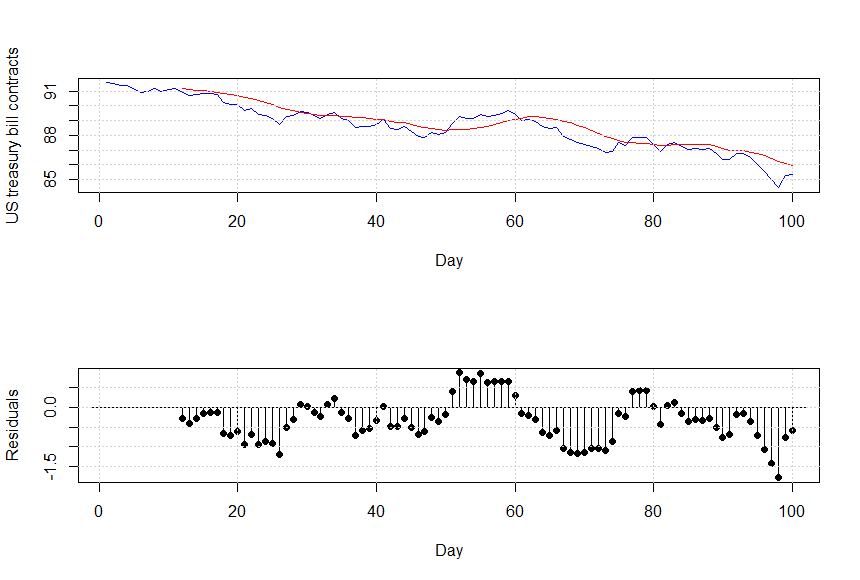
\includegraphics[width=0.7\textwidth]{biased.png}	
			\end{center}			
		\end{itemize}			
	}
	
	\only<2>{
%%%%%%%%%%%%%%%%%%%%%%%%%%%%%%%%%%%%%%%%%%%%%%%%%%%%%%%%%%%%%%%%%%%%%%%			
% Ряд перед вами спрогнозирован наивным методом - "завтра будет то же, что сегодня". Для рядов с выраженной сезонностью такой метод прогнозирования даёт не самые лучшие результаты: как видно на ACF, остатки оказываются автокоррелированными, то есть, в них остаётся ещё какая-то структура, которую можно попытаться учесть при прогнозировании.
% Автокоррелированность остатков — признак того, что в данных присутствует информация, которая не вошла в модель. Если в остатках есть структура, то можно попытаться её внести в модель явным образом. Скорректированная модель будет лучше, а её остатки будут больше похожи на белый шум. Однако это можно сделать далеко не всегда — возможности моделей не безграничны, и с их помощью иногда нельзя учесть всю структуру ряда. Таким образом, автокоррелированность остатков только указывает на потенциальную возможность улучшить модель, и не факт, что улучшения можно добиться на практике с помощью рассматриваемого класса моделей.
%%%%%%%%%%%%%%%%%%%%%%%%%%%%%%%%%%%%%%%%%%%%%%%%%%%%%%%%%%%%%%%%%%%%%%%			
		\begin{itemize}
			\item Неавтокоррелированность~--- отсутствие неучтённой зависимости от~предыдущих наблюдений:
			\begin{center}
				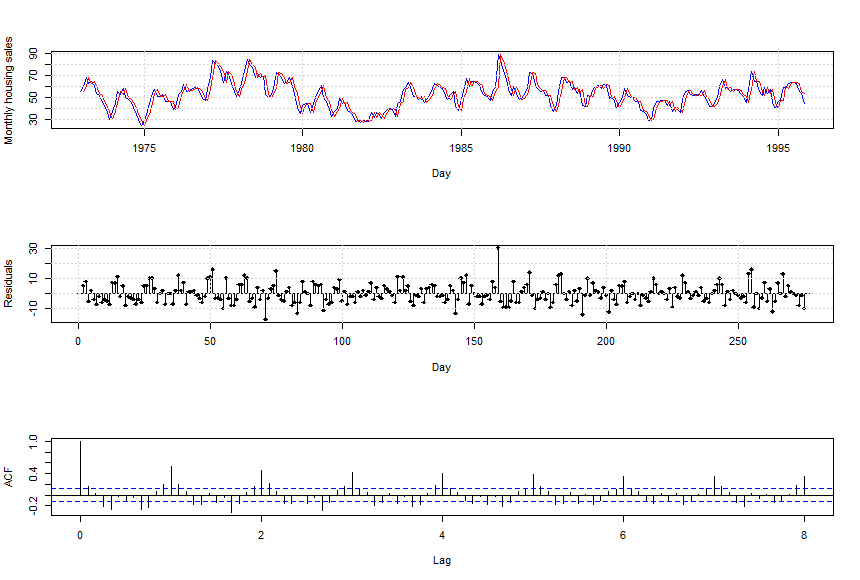
\includegraphics[width=0.7\textwidth]{autocorrelated.png}			
			\end{center}	
		\end{itemize}
	}	
    \end{frame}

    
\begin{frame}{Q-критерий Льюнга-Бокса}
%%%%%%%%%%%%%%%%%%%%%%%%%%%%%%%%%%%%%%%%%%%%%%%%%%%%%%%%%%%%%%%%%%%%%%%			
% Критерий Льюнга-Бокса позволяет проверить гипотезу о том, что автокорреляция равна нулю сразу при всех лагах от 1 до L. Статистика представляет собой взвешенную сумму выборочных автокорреляций.
%%%%%%%%%%%%%%%%%%%%%%%%%%%%%%%%%%%%%%%%%%%%%%%%%%%%%%%%%%%%%%%%%%%%%%%	
	\begin{center}
		\begin{tabular}{rl}
			ряд ошибок прогноза:            & $\varepsilon^T = \varepsilon_1,\dots,\varepsilon_T;$ \\
			нулевая гипотеза:               & $H_0\colon r_1 = \dots = r_L=0;$ \\
			альтернатива:                   & $H_1\colon H_0$ неверна;\\
			статистика:                     & $Q\left(\varepsilon^T\right) = T\left(T+2\right) \sum\limits_{\tau=1}^L \frac{r_{\tau}^2}{T-\tau};$ \\
			нулевое распределение:          & $\chi^2_{L-K}$, $K$~--- число настраиваемых\\
			& параметров модели ряда.
		\end{tabular}
		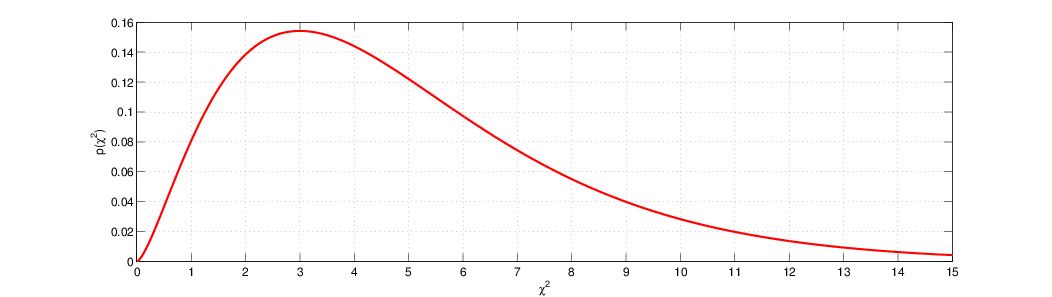
\includegraphics[width=0.8\textwidth]{chi2.png}
	\end{center}
\end{frame}
    
\begin{frame}

%%%%%%%%%%%%%%%%%%%%%%%%%%%%%%%%%%%%%%%%%%%%%%%%%%%%%%%%%%%%%%%%%%%%%%%			
% Если остатки смещены, это значит, что пронозы станут в среднем лучше, если добавить к ним константу, на которую проиходит смещение. Ряд перед вами мы попробовали спрогнозировать наивным сезонным методом, когда в качестве прогноза выбирается значение ряда в предыдущий такой же сезон. Такой прогноз оказывается смещённым, поэтому мы его корректируем на константу. Однако, это делает остатки нестационарными: несмотря на то, что в среднем по периоду смещения нет, прогнозные значения в начале периода оказываются заниженными, в конце - завышенными.
%%%%%%%%%%%%%%%%%%%%%%%%%%%%%%%%%%%%%%%%%%%%%%%%%%%%%%%%%%%%%%%%%%%%%%%			
		\begin{itemize}
			\item Стационарность~--- отсутствие зависимости от времени:
			\begin{center}
				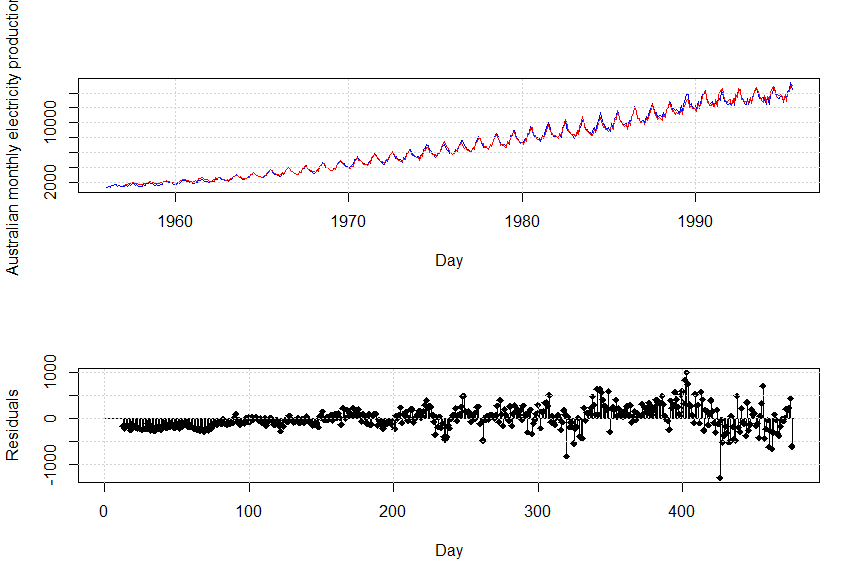
\includegraphics[width=0.6\textwidth]{trended.png}			
			\end{center}		
		\end{itemize}		
		
\end{frame}

\begin{frame}{Желательные свойства остатков прогноза}
		\begin{itemize}
			\item Нормальность:
			\begin{center}
				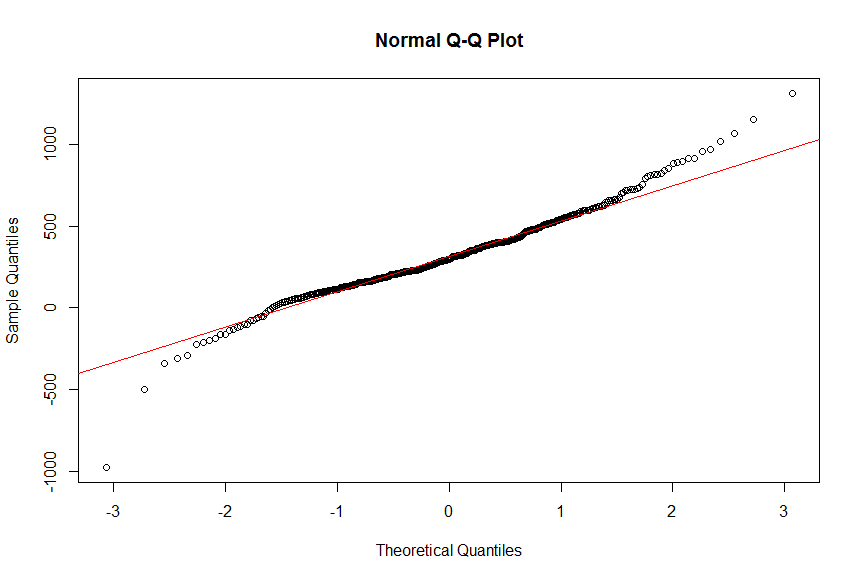
\includegraphics[width=0.6\textwidth]{qqplot.png}			
			\end{center}		
		\end{itemize}	
\end{frame}

\begin{frame}{Проверка свойств остатков}
	\begin{itemize}
		\item Несмещённость~--- критерий Стьюдента или Уилкоксона.
		\item Стационарность~--- визуальный анализ, критерий KPSS.
		\item Неавтокоррелированность~--- коррелограмма, Q-критерий Льюнга-Бокса.
		\item Нормальность~--- q-q plot, критерий Шапиро-Уилка.
	\end{itemize}
\end{frame}



\begin{frame}{Простейшие методы прогнозирования}
	\begin{itemize}
		\item средним:
		$$\hat{y}_{T+d} = \frac1{T}\sum_{t=1}^T y_t;$$
		\item средним за последние $k$ отсчётов:
		$$\hat{y}_{T+d} = \frac1{k}\sum_{t=T-k}^T y_t;$$
		\item наивный:
		$$\hat{y}_{T+d} = y_T;$$
		\item наивный сезонный ($s$~--- период сезонности):
		$$\hat{y}_{T+d} = y_{T+d-ks}, \; k = \lfloor\left(d-1\right)/s\rfloor+1;$$
		\item экстраполяции тренда:
		$$\hat{y}_{T+d} = y_T + d \frac{y_T-y_1}{T-1}.$$
	\end{itemize}
\end{frame}





\section{Модели семейства ЭСС}
\subsection{Частные случаи}
\begin{frame}{Простое экспоненциальное сглаживание (метод Брауна)}
	\only<1>{
		Наивный прогноз: $$\hat{y}_{T+1|T} = y_T.$$
		Прогноз средним значением: $$\hat{y}_{T+1|T} = \sum_{t=1}^T y_t.$$
		Прогноз с помощью взвешенного среднего с экспоненциально убывающими весами:
		$$\hat{y}_{T+1|T} = \alpha y_T + \alpha \left(1-\alpha\right)y_{T-1} + \alpha \left(1-\alpha\right)^2y_{T-2}+\dots$$
		$\alpha \uparrow 1 \; \Rightarrow$ больший вес последним точкам,
		
		$\alpha \downarrow 0 \; \Rightarrow$ большее сглаживание.
		
		\bigskip
		
		{\footnotesize
			\begin{table}[h]
				\begin{tabular}{|c|c|c|c|c|}
					\hline
					Наблюдение & $\alpha=0.2$ & $\alpha=0.4$ & $\alpha=0.6$ & $\alpha=0.8$ \\\hline
					$y_T$      & $0.2$        & $0.4$        & $0.6$        & $0.8$        \\
					$y_{T-1}$  & $0.16$       & $0.24$       & $0.24$       & $0.16$       \\
					$y_{T-2}$  & $0.128$      & $0.144$      & $0.096$      & $0.032$      \\
					$y_{T-3}$  & $0.1024$     & $0.0864$     & $0.0384$     & $0.0064$     \\
					$y_{T-4}$  & $0.08192$    & $0.05184$    & $0.01536$    & $0.00128$    \\
					$y_{T-5}$  & $0.065536$   & $0.031104$   & $0.006144$   & $0.000256$   \\
					\hline
				\end{tabular}
			\end{table}	
		}	
	}
	
	\only<2>{
		\begin{itemize}
			\item Метод подходит для прогнозирования рядов без тренда и сезонности:
			\begin{align*}
			\hat{y}_{t+1|t} &= l_t, \\
			l_t &= \alert{\alpha} y_t + \alert{\left(1-\alpha\right)}l_{t-1}=\hat y_{t|t-1} + \alert{\alpha\cdot e_t}.
			\end{align*}
%    \[
%        \hat y_{t+1} := \alert{\alpha} y_t + \alert{(1-\alpha)} \hat y_{t}= \hat y_{t} + \alert{\alpha\cdot e_t}
%    \]
%
    $e_t = y_t-\hat{y}_{t|t-1}$~--- ошибка прогноза отсчёта времени $t$


			\item Прогноз зависит от $l_0$:
			$$\hat{y}_{T+1|T} = \sum_{j=1}^{T-1}\alpha\left(1-\alpha\right)^j y_{T-j} + \left(1-\alpha\right)^T l_0.$$
			Можно взять $l_0=y_1$ или оптимизировать его.
			\item Прогноз получается плоский, т.\,е. $\hat{y}_{t+d|t} = \hat{y}_{t+1|t}$.
		\end{itemize}
	}	
	
	\only<3>{
		\begin{center}
			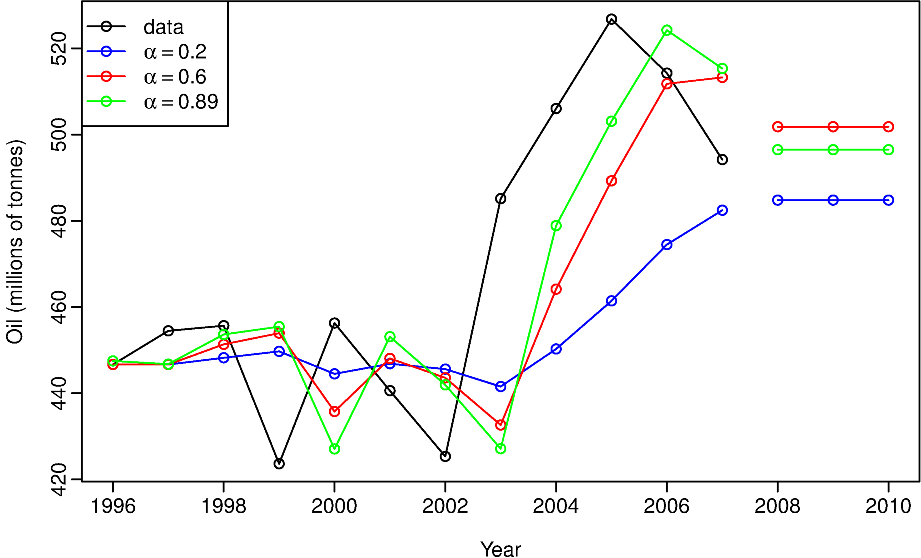
\includegraphics[width=0.6\textwidth]{fig_7_ses}
		\end{center}
		Простое экспоненциальное сглаживание в применении к данным о добыче нефти в Саудовской Аравии (1996–2007).
	}
\end{frame}

\begin{frame}{Методы, учитывающие тренд}
	\only<1>{
		Аддитивный линейный тренд (метод Хольта):
		\begin{align*}
		\hat{y}_{t+d|t} &= l_t + d b_t, \\
		l_{t}       &= \alpha y_t + \left(1-\alpha\right) \left(l_{t-1} + b_{t-1}\right), \\
		b_t         &= \beta \left(l_t - l_{t-1}\right) + \left(1-\beta\right) b_{t-1}.
		\end{align*}
		
		\bigskip
		
		Мультипликативный линейный (экспоненциальный) тренд:
		\begin{align*}
		\hat{y}_{t+d|t} &= l_tb_t^d, \\
		l_{t}       &= \alpha y_t + \left(1-\alpha\right) \left(l_{t-1} b_{t-1}\right), \\
		b_t         &= \beta \frac{l_t}{l_{t-1}} + \left(1-\beta\right) b_{t-1}.
		\end{align*}
		
		\bigskip
		
		$\alpha, \beta \in \left[0,1\right].$
	}
	
	\only<2>{
		Аддитивный затухающий тренд:
		\begin{align*}
		\hat{y}_{t+d|t} &= l_t + \left(\phi + \phi^2 + \dots + \phi^{d}\right) b_t, \\
		l_{t}       &= \alpha y_t + \left(1-\alpha\right) \left(l_{t-1} +\phi b_{t-1}\right), \\
		b_t         &= \beta \left(l_t - l_{t-1}\right) + \left(1-\beta\right)\phi b_{t-1}.
		\end{align*}
		
		\bigskip
		
		Мультипликативный затухающий тренд:
		\begin{align*}
		\hat{y}_{t+d|t} &= l_t b_t^{\left(\phi + \phi^2 + \dots + \phi^{d}\right)}, \\
		l_{t}       &= \alpha y_t + \left(1-\alpha\right) l_{t-1} b_{t-1}^{\phi}, \\
		b_t         &= \beta\frac{l_t}{l_{t-1}} + \left(1-\beta\right)b_{t-1}^{\phi}.
		\end{align*}
		
		\bigskip
		
		$\alpha, \beta \in \left[0,1\right], \; \phi \in \left(0,1\right).$
	}
	
	\only<3>{
		\begin{center}
			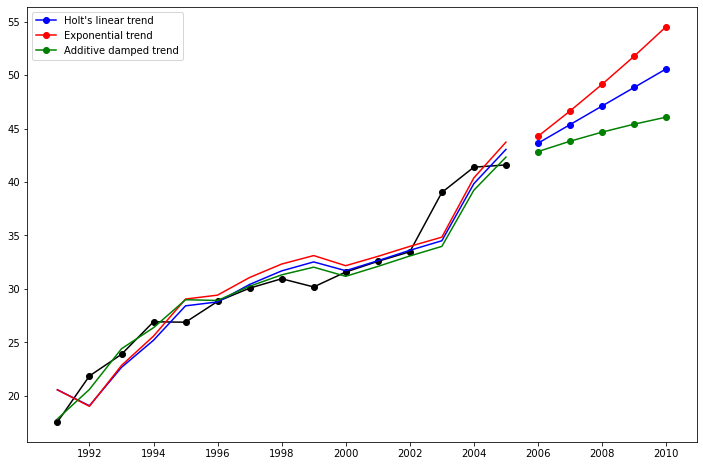
\includegraphics[width=0.5\textwidth]{fig_7_from_statsmodels.png}
		\end{center}
		Прогнозы поголовья овец в Азии с учётом тренда.
		

		}
	
\end{frame}

\begin{frame}{Методы, учитывающие сезонность}
	\only<1>{
		Аддитивная сезонность c периодом длины $m$ (метод Тейла-Веджа):
		\begin{align*}
		\hat{y}_{t+d|t} &= l_t + d b_t + s_{t-m+\left(d \mod m\right)}, \\
		l_{t}       	&=  \alpha \left(y_t - s_{t-m}\right)+ \left(1-\alpha\right) \left(l_{t-1} + b_{t-1}\right), \\
		b_t         	&= \beta \left(l_t - l_{t-1}\right) + \left(1-\beta\right)b_{t-1}, \\
		s_t         	&= \gamma\left(y_t-l_{t-1}-b_{t-1}\right) + \left(1-\gamma\right)s_{t-m}.
		\end{align*}
		
		\bigskip
		
		Мультипликативная сезонность (Хольта-Уинтерса):
		\begin{align*}
		\hat{y}_{t+d|t} &= \left(l_t + d b_t\right)s_{t-m+\left(d \mod m\right)}, \\
		l_{t}           &= \alpha \frac{y_t}{s_{t-m}}+ \left(1-\alpha\right) \left(l_{t-1} + b_{t-1}\right), \\
		b_t             &= \beta \left(l_t - l_{t-1}\right) + \left(1-\beta\right)b_{t-1}, \\
		s_t             &= \gamma\frac{y_t}{l_{t-1}+b_{t-1}} + \left(1-\gamma\right)s_{t-m}.
		\end{align*}
	}
	
	
	\only<2>{
		\begin{center}
			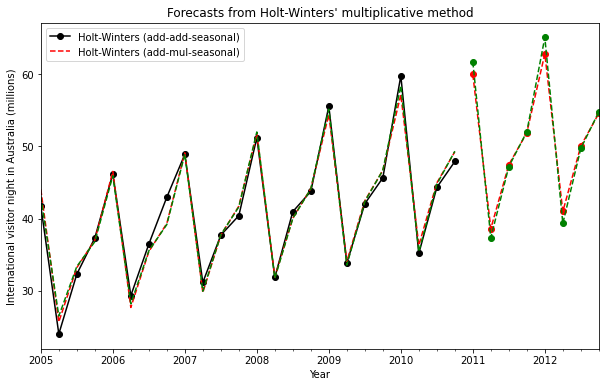
\includegraphics[width=0.5\textwidth]{fig_7_2.png}
		\end{center}
		Прогнозы с учётом тренда и сезонности количества ночей, проведённых туристами в Австралии.
	}
	
		\only<3>{
		\begin{center}
			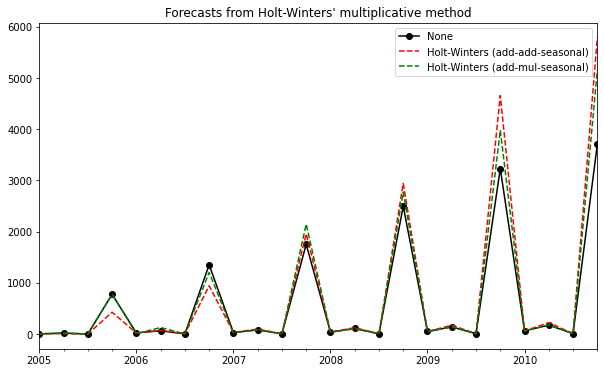
\includegraphics[width=0.35\textwidth]{season_hw1.png}
			
            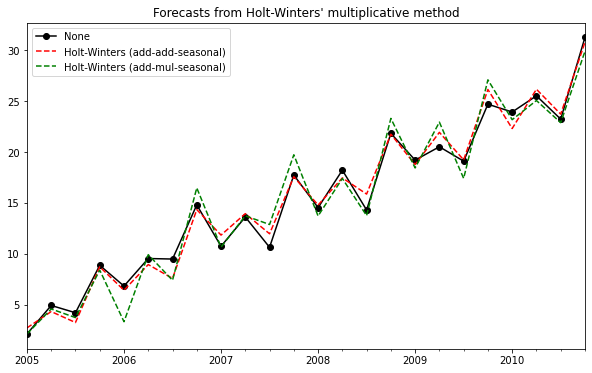
\includegraphics[width=0.35\textwidth]{season_hw2.png}
		\end{center}

	}
	
\end{frame}

\begin{frame}{Скользящее среднее}
%%%%%%%%%%%%%%%%%%%%%%%%%%%%%%%%%%%%%%%%%%%%%%%%%%%%%%%%%%%%%%%%%%%%%%%			
% Следующий класс моделей — это скользящее среднее. Чтобы лучше понимать, как они устроены, можно начать с рассмотрения независимого, одинаково распределённого во времени шума. Для каждого значения t можно вычислить среднее арифметическое между точками t и t-1. Также можно вычислять среднее не по двум, а по трём или четырём точкам. То, что получается в результате такого усреднения, — это уже не простая выборка с независимыми, одинаково распределёнными элементами. Соседние значения на красной линии очень похожи друг на друга, потому что в их вычислении используются одни и те же шумовые компоненты.
%%%%%%%%%%%%%%%%%%%%%%%%%%%%%%%%%%%%%%%%%%%%%%%%%%%%%%%%%%%%%%%%%%%%%%%			
	\only<1>{	
		Пусть у нас есть независимый одинаково распределённый во времени шум $\varepsilon_t$:
		\begin{center}
			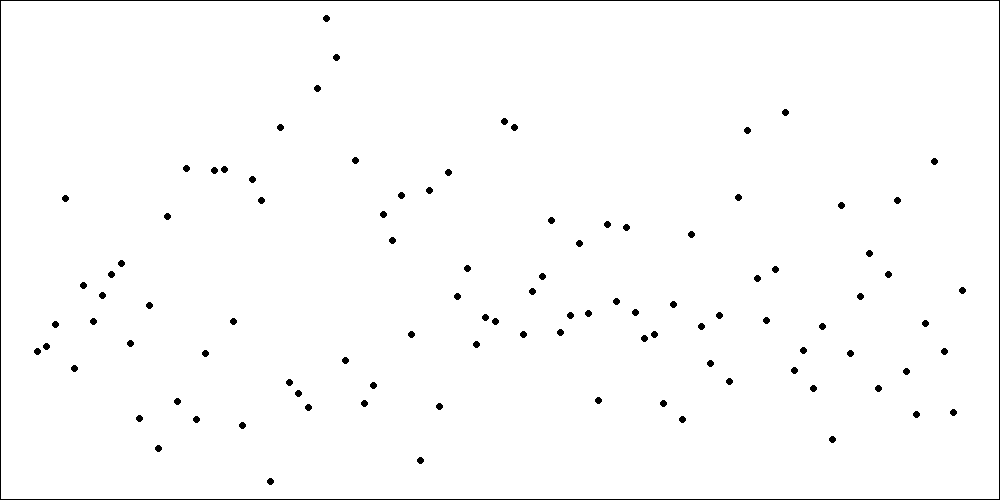
\includegraphics[width=0.8\textwidth]{MA1.png}
		\end{center}	
	}
	\only<2>{
		Среднее по двум соседним точкам:
		\begin{center}
			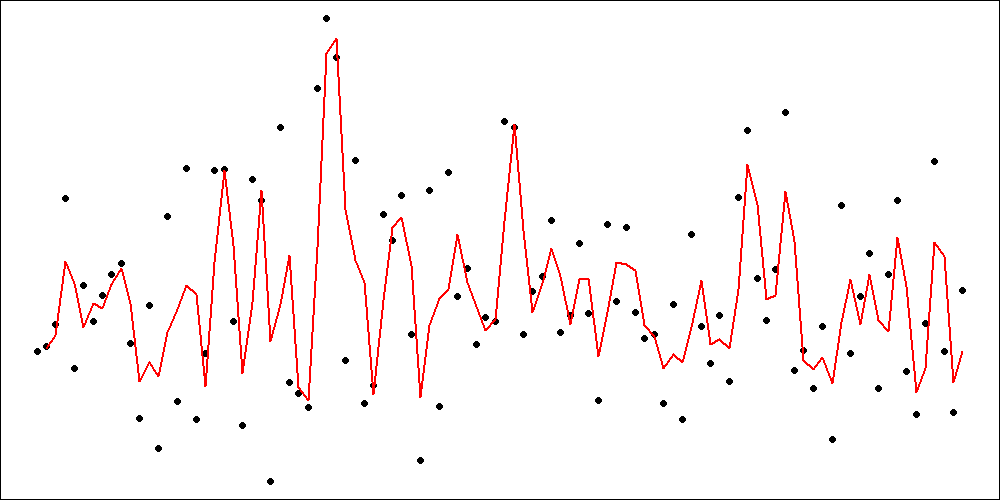
\includegraphics[width=0.8\textwidth]{MA2.png}
		\end{center}	
	}
	\only<3>{
		Среднее по трём соседним точкам:
		\begin{center}
			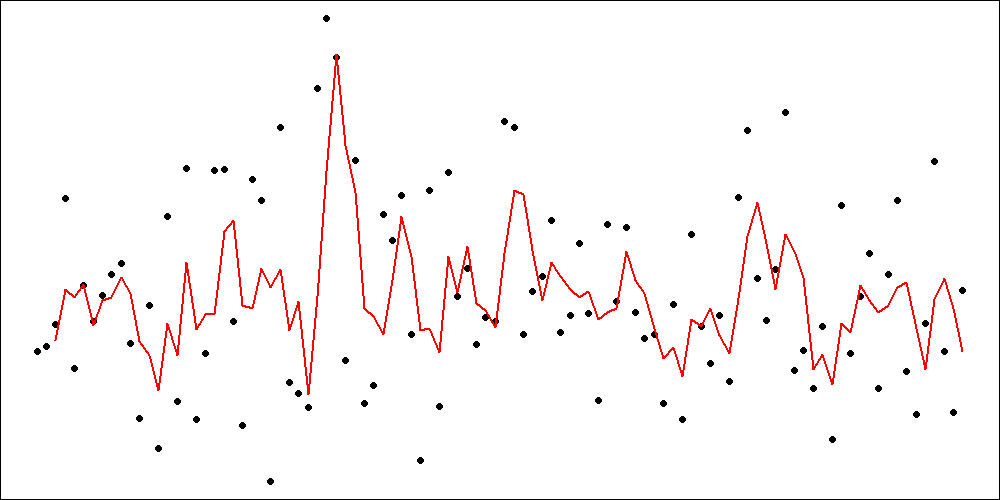
\includegraphics[width=0.8\textwidth]{MA3.png}
		\end{center}	
	}
	\only<4>{
		Среднее по четырём соседним точкам:
		\begin{center}
			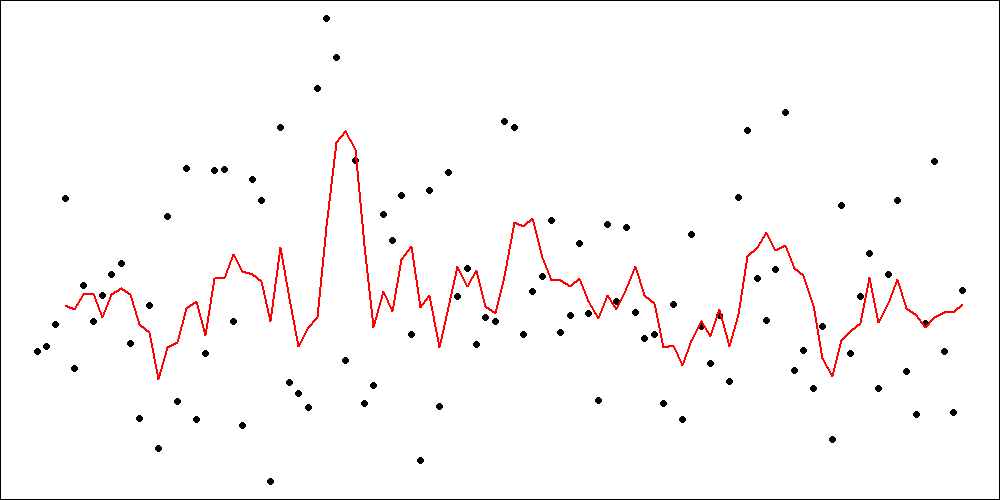
\includegraphics[width=0.8\textwidth]{MA4.png}
		\end{center}	
	}
	\end{frame}



\begin{frame}{Авторегрессия}
%%%%%%%%%%%%%%%%%%%%%%%%%%%%%%%%%%%%%%%%%%%%%%%%%%%%%%%%%%%%%%%%%%%%%%%			
% Ранее была предпринята попытка свести задачу прогнозирования временного ряда к задаче регрессии, выбирая какие-то признаки, зависящие от времени. Результат получился плохим, выбранных признаков явно недостаточно, нужны дополнительные. Можно перейти к следующей идее: делать регрессию для ряда не на какие-то внешние признаки, зависящие от времени, а на его собственные значения в прошлом. Такая модель называется моделью авторегрессии порядка p (AR(p)). В этой модели yt представляет собой линейную комбинацию p предыдущих значений ряда и шумовой компоненты.
%%%%%%%%%%%%%%%%%%%%%%%%%%%%%%%%%%%%%%%%%%%%%%%%%%%%%%%%%%%%%%%%%%%%%%%			
%    \only<1>{
    $$AR(p)\colon \;\;\; y_t = \phi_1 y_{t-1} + \phi_2 y_{t-2} + \dots + \phi_p y_{t-p} + \varepsilon_t,$$
    где $y_t$~--- стационарный ряд с нулевым средним, $\phi_1,\dots,\phi_p$~--- константы ($\phi_p \neq 0$), $\varepsilon_t$~--- гауссов белый шум с нулевым средним и постоянной дисперсией $\sigma_\varepsilon^2.$

    \bigskip

    Если среднее равно $\mu$, модель принимает вид
    $$y_t = \alpha + \phi_1y_{t-1} + \phi_2 y_{t-2} + \dots + \phi_p y_{t-p} + \varepsilon_t,$$
    где $\alpha=\mu\left(1-\phi_1-\dots-\phi_p\right).$

    \bigskip

    Другой способ записи:
    $$\phi\left(B\right)y_t = \left(1-\phi_1B - \phi_2B^2 - \dots - \phi_pB^p\right)y_t = \varepsilon_t,$$
    где $B$~--- разностный оператор ($By_t = y_{t-1}$).

    \bigskip

    Линейная комбинация $p$ подряд идущих членов ряда даёт белый шум.
%	}
%	
%	\only<2>{
%	Чтобы ряд AR(p) был стационарным, должны выполняться ограничения на коэффициенты.
%	Например,
%	\begin{itemize}
%		\item в AR(1) необходимо $-1<\phi_1<1$;
%		\item в AR(2) необходимо $-1<\phi_2<1, \;\phi_1+\phi_2<1,\; \phi_2-\phi_1<1$.
%	\end{itemize}
%	C ростом $p$ вид ограничений усложняется.		
%	}
\end{frame}

\section{ARIMA}
\subsection{Теория}

\begin{frame}{ARMA (Autogerressive moving average)}
%%%%%%%%%%%%%%%%%%%%%%%%%%%%%%%%%%%%%%%%%%%%%%%%%%%%%%%%%%%%%%%%%%%%%%%			
% Можно проделать следующий трюк: взять авторегрессионную модель порядка p и модель скользящего среднего порядка q и сложить то, что находится у них в правых частях. Результат — это модель ARMA(p, q). Главное, что нужно знать об этой модели: теорема Вольда утверждает, что любой стационарный временной ряд может быть описать моделью ARMA(p; q) с правильным подбором значений параметров p; q. Это прекрасный результат, который означает, что семейство моделей ARMA(p; q) достаточно богато для того, чтобы в нём можно было найти хорошую модель, описывающую любой стационарный ряд.
%%%%%%%%%%%%%%%%%%%%%%%%%%%%%%%%%%%%%%%%%%%%%%%%%%%%%%%%%%%%%%%%%%%%%%%			
    $$ARMA(p,q)\colon \;\; y_t = \phi_1 y_{t-1} + \dots + \phi_p y_{t-p} + \varepsilon_t + \theta_1\varepsilon_{t-1} + \theta_2\varepsilon_{t-2} + \dots + \theta_q \varepsilon_{t-q},$$
    где $y_t$~--- стационарный ряд с нулевым средним, $\phi_1,\dots,\phi_p,\theta_1,\dots,\theta_q$~--- константы ($\phi_p \neq 0$, $\theta_q\neq0$), $\varepsilon_t$~--- гауссов белый шум с нулевым средним и~постоянной дисперсией $\sigma_\varepsilon^2.$

    \bigskip

    Если среднее равно $\mu$, модель принимает вид
    $$y_t = \alpha + \phi_1y_{t-1} + \phi_2 y_{t-2} + \dots + \phi_p y_{t-p} + \varepsilon_t + \theta_1\varepsilon_{t-1} + \theta_2\varepsilon_{t-2} + \dots + \theta_q \varepsilon_{t-q},$$
    где $\alpha=\mu\left(1-\phi_1-\dots-\phi_p\right).$

    \bigskip

    Другой способ записи:
    $$\phi\left(B\right)y_t = \theta\left(B\right)\varepsilon_t.$$

    \bigskip

    Теорема Вольда: любой стационарный ряд может быть аппроксимирован моделью $ARMA(p,q)$ с любой точностью.
\end{frame}

\begin{frame}{ARIMA (Autogerressive integrated moving average)}
%%%%%%%%%%%%%%%%%%%%%%%%%%%%%%%%%%%%%%%%%%%%%%%%%%%%%%%%%%%%%%%%%%%%%%%			
% 1. Теорема Вольда: любой стационарный ряд может быть описан моделью ARMA(p; q) с любой наперёд заданной точностью.
% 2. При помощи дифференцирования нестационарный ряд можно сделать стационарным.
% Эти две идеи и лежат в основе моделей класса ARIMA. Модель ARIMA(p; d; q) — это модель ARMA(p; q) для d раз продифференцированного ряда.
%%%%%%%%%%%%%%%%%%%%%%%%%%%%%%%%%%%%%%%%%%%%%%%%%%%%%%%%%%%%%%%%%%%%%%%			
    Ряд описывается моделью $ARIMA(p,d,q),$ если ряд его разностей $$\nabla^d y_t = \left(1-B\right)^d y_t$$ описывается моделью $ARMA(p,q)$.

    $$\phi\left(B\right)\nabla^d y_t = \theta\left(B\right)\varepsilon_t.$$
\end{frame}

\subsection{Определение параметров моделей}
\begin{frame}{$\alpha, \phi, \theta$}
%%%%%%%%%%%%%%%%%%%%%%%%%%%%%%%%%%%%%%%%%%%%%%%%%%%%%%%%%%%%%%%%%%%%%%%			
% После изучения устройства моделей класса ARIMA настало время разобраться, как настраивать эти модели и получать с их помощью прогнозы. У моделей класса ARIMA есть несколько групп параметров. Параметры d;D; q; Q; p; P можно считать гиперпараметрами, поскольку они определяют структуру и количество коэффициентов в самой модели ARIMA. Остальные параметры являются коэффициентами в регрессионном уравнении.
% Если зафиксированы параметры d;D; q; Q; p; P, то есть зафиксирована структура модели ARIMA, то остальные параметры  можно подобрать с помощью метода наименьших квадратов. Фактически происходит настраивание привычной регрессии методом минимизации квадратичной ошибки.
% Единственный трюк заключается в определении коэффициентов тета, которые стоят при шумовых компонентах из прошлого. Наблюдать шумовые компоненты невозможно, поэтому, чтобы подставить их в регрессионное уравнение, их нужно предварительно оценить. Обычно оценка производится с помощью остатков от авторегрессии, которая предварительно строится по исследуемым данным.
% Если шум, который стоит в модели ARIMA, является белым (независимый, одинаково распределённый, гауссовский), то метод наименьших квадратов даёт оценки максимального правдоподобия для параметров альфа, фи и тета, а, значит, эти оценки обладают некоторыми хорошими свйоствами.
%%%%%%%%%%%%%%%%%%%%%%%%%%%%%%%%%%%%%%%%%%%%%%%%%%%%%%%%%%%%%%%%%%%%%%%			
	\begin{itemize}
		\item Если все остальные параметры фиксированы, коэффициенты регрессии подбираются методом наименьших квадратов
		\item Чтобы найти коэффициенты $\theta$, шумовая компонента предварительно оценивается с помощью остатков авторегрессии
		\item Если шум белый (независимый одинаково распределённый гауссовский), то МНК даёт оценки максимального правдоподобия
	\end{itemize}
\end{frame}

\begin{frame}{$d, D$}
%%%%%%%%%%%%%%%%%%%%%%%%%%%%%%%%%%%%%%%%%%%%%%%%%%%%%%%%%%%%%%%%%%%%%%%			
% Параметры d;D, которые задают порядки дифференцирования, необходимо подбирать так, чтобы ряд стал стационарным. Ранее уже упоминалось, что всегда рекомендуется начинать с сезонного дифференцирования, потому что уже после него ряд может оказаться стационарным. Дело в том, что выгодно дифференцировать ряд как можно меньше раз, потому что с увеличением количества дифференцирований растёт дисперсия итогового прогноза.
%%%%%%%%%%%%%%%%%%%%%%%%%%%%%%%%%%%%%%%%%%%%%%%%%%%%%%%%%%%%%%%%%%%%%%%			
	\begin{itemize}
		\item Порядки дифференцирования подбираются так, чтобы ряд стал стационарным
		\item Ещё раз: если ряд сезонный, рекомендуется начинать с сезонного дифференцирования
		\item Чем меньше раз мы продифференцируем, тем меньше будет дисперсия итогового прогноза
	\end{itemize}
\end{frame}

\begin{frame}{$q, Q, p, P$}
%%%%%%%%%%%%%%%%%%%%%%%%%%%%%%%%%%%%%%%%%%%%%%%%%%%%%%%%%%%%%%%%%%%%%%%			
% К сожалению, гиперпараметры q; Q; p; P нельзя выбирать из принципа максимума правдоподобия. Например, чем больше значение параметра p, тем больше авторегрессионных компонент в итоговом уравнении, тем больше параметров фи и тем лучше это уравнение описывает данные. Чем больше значения гиперпараметров, тем больше параметров в модели и тем она сложнее. Таким образом, с увеличением значения этих гиперпараметров значение правдоподобия может только увеличиваться. Поэтому для сравнения моделей с разным количеством параметров необходим другой критерий, например, критерий Акаике.
% Оптимальной по критерию Акаике будет модель с наименьшим значением этого критерия. Такая модель, с одной стороны, будет достаточно хорошо описывать данные, а с другой — содержать не слишком большое количество параметров. В конечном итоге значения параметров q; Q; p; P определяются перебором: из разных значений гиперпараметров выбираются те, у которых значение критерия Акаике будет минимальным. Начальные приближения для этого перебора можно выбрать с помощью автокорреляционной функции.
%%%%%%%%%%%%%%%%%%%%%%%%%%%%%%%%%%%%%%%%%%%%%%%%%%%%%%%%%%%%%%%%%%%%%%%			
	\begin{itemize}
		\item Гиперпараметры нельзя выбирать из принципа максимума правдоподобия: $L$~всегда увеличивается с~их ростом
		\item Для сравнения моделей с разными $q, Q, p, P$ можно использовать информационные критерии
		\item Начальные приближения можно выбрать с помощью автокорреляций
	\end{itemize}
\end{frame}

\begin{frame}{Автокорреляционная функция (ACF)}
%%%%%%%%%%%%%%%%%%%%%%%%%%%%%%%%%%%%%%%%%%%%%%%%%%%%%%%%%%%%%%%%%%%%%%%
% Одной из важнейших характеристик временного ряда является автокорреляция, измеряющая в каком-то смысле сходство между значениями ряда в соседних точках. Автокорреляция — это уже встречавшаяся ранее корреляция Пирсона между исходным рядом и его версией, сдвинутой на несколько отсчётов. Количество отсчётов, на которое сдвинут ряд, называется лагом автокорреляции. Значения, принимаемые автокорреляцией такие же, как и у коэффициента Пирсона: [-1; 1]. Проверить, значимо ли отличие автокорреляции от нуля, можно с помощью такого же критерия Стьюдента, как используется для корреляции Пирсона.
%%%%%%%%%%%%%%%%%%%%%%%%%%%%%%%%%%%%%%%%%%%%%%%%%%%%%%%%%%%%%%%%%%%%%%%
	\only<1>{
	Наблюдения временного ряда автокоррелированы.
	
	\bigskip	
		
		\textbf{Автокорреляция:}
		$$r_\tau = r_{y_t y_{t+\tau}} = \frac{\sum\limits_{t=1}^{T-\tau} \left(y_t - \bar{y}\right)\left(y_{t+\tau} - \bar{y}\right) }{ \sum\limits_{t=1}^T \left(y_t - \bar{y}\right)^2 },\;\; \bar{y} = \frac1{T} \sum_{t=1}^T y_t.$$
		
		$r_\tau \in\left[-1,1\right], \;\; \tau$~--- лаг автокорреляции.
		
		\bigskip
		
		Проверка значимости отличия автокорреляции от нуля:
		\begin{center}
			\begin{tabular}{rl}
				временной ряд:                  & $Y^T = Y_1,\dots,Y_T;$ \\
				нулевая гипотеза:               & $H_0\colon r_\tau=0;$ \\
				альтернатива:                   & $H_1\colon r_\tau\neq0;$ \\
				статистика:                     & $T\left(Y^T\right) = \frac{r_{\tau} \sqrt{T-\tau-2}}{\sqrt{1-r_\tau^2}};$ \\
				нулевое распределение:          & $St\left(T-\tau-2\right)$.\\
			\end{tabular}
		\end{center}
	}
	
			
	
\end{frame}


\begin{frame}{Частичная автокорреляционная функция (PACF)}
	\textbf{Частичная автокорреляция} стационарного ряда $y_t$~--- автокорреляция остатков авторегрессии предыдущего порядка:
	$$\phi_{hh} = \begin{cases}
	r\left(y_{t+1},y_t\right), & h=1, \\
	r\left(y_{t+h} - \hat{y}_{t+h}, y_{t} - \hat{y}_t\right), & h\geq 2,
	\end{cases}
	$$
	где $\hat{y}_{t+h}$ и $\hat{y}_{t}$~--- предсказания регрессий $y_{t+h}$ и $y_{t}$ на $y_{t+1}, y_{t+2}, \dots, y_{t+h-1}$:
	\begin{align*}
	\hat{y}_t     &= \beta_1y_{t+1} +\beta_2y_{t+2} + \dots + \beta_{h-1} y_{t+h-1}, \\
	\hat{y}_{t+h} &= \beta_1y_{t+h-1} +\beta_2y_{t+h-2} + \dots + \beta_{h-1} y_{t+1}. \\
	\end{align*}	
\end{frame}

\begin{frame}{$q, Q, p, P$}
\begin{itemize}
	\item В модели $ARIMA(p,d,0)$ ACF экспоненциально затухает или имеет синусоидальный вид, а PACF значимо отличается от нуля при лаге $p$
	\item В модели $ARIMA(0,d,q)$ PACF экспоненциально затухает или имеет синусоидальный вид, а ACF значимо отличается от нуля при лаге $q$
\end{itemize}

$\Rightarrow$ начальные приближения для $p,q,P,Q$:

\begin{itemize}
	\item $q$: номер последнего лага $\tau<S$, при котором автокорреляция значима	
	\item $p$: номер последнего лага $\tau<S$, при котором частичная автокорреляция значима		
\end{itemize}
\end{frame}

\subsection{Прогнозирование}
\begin{frame}{Прогнозирование с помощью ARIMA}
	\only<1>{
		\begin{enumerate}
			\item Строится график ряда, идентифицируются необычные значения.
			\item При необходимости делается стабилизирующее дисперсию преобразование.
			\item Если ряд нестационарен, подбирается порядок дифференцирования.
			\item Анализируются ACF/PACF, чтобы понять, можно ли использовать модели AR(p)/MA(q).
			\item Обучаются модели-кандидаты, сравнивается их AIC/AICc.
			\item Остатки полученной модели исследуются на несмещённость, стационарность и неавтокоррелированность; если предположения не~выполняются, исследуются модификации модели.
			\item В финальной модели $t$ заменяется на $T+h$, будущие наблюдения~--- на их прогнозы, будущие ошибки~--- на нули, прошлые ошибки~--- на~остатки.
		\end{enumerate}
	}
\end{frame}

\section{}
\begin{frame}{Литература}
	Hyndman R.J., Athanasopoulos G. \textit{Forecasting: principles and practice}. --- OTexts, \url{https://www.otexts.org/book/fpp}
\end{frame}
\end{document}
